\synctex=1
\documentclass[a4paper,11pt,svgnames]{book}

\usepackage[utf8x]{inputenc}
\usepackage{mathtools}
\usepackage{thesis}
\usepackage{calc}
\usepackage{float}
\usepackage{acronym}
\usepackage{siunitx}
\usepackage{eurosym}
\usepackage[titletoc]{appendix}

% \setlength{\marginparwidth}{2cm}
% \setlength{\voffset}{-0.25in}
\setlength{\parskip}{0.1in}

% \usepackage{draftwatermark}
% \SetWatermarkScale{4}
\usepackage{subfig}
\usepackage{listings}
\usepackage{courier}
\usepackage{enumitem}
% \usepackage{indentfirst}

\lstset{
    basicstyle=\footnotesize\ttfamily,
    numbers=none,               % Ort der Zeilennummern
    numberstyle=\tiny,          % Stil der Zeilennummern
    % stepnumber=2,               % Abstand zwischen den Zeilennummern
    numbersep=5pt,              % Abstand der Nummern zum Text
    tabsize=2,                  % Groesse von Tabs
    extendedchars=true,         %
    breaklines=true,            % Zeilen werden Umgebrochen
    % keywordstyle=\color{red},
    frame=single,         
    % keywordstyle=[1]\textbf,    % Stil der Keywords
    % keywordstyle=[2]\textbf,    %
    % keywordstyle=[3]\textbf,    %
    % keywordstyle=[4]\textbf,   \sqrt{\sqrt{}} %
    % stringstyle=\color{white}\ttfamily, % Farbe der String
    showspaces=false,           % Leerzeichen anzeigen ?
    showtabs=false,             % Tabs anzeigen ?
    belowcaptionskip=12pt,
    xleftmargin=2em, 
    xrightmargin=4pt,
    % backgroundcolor=\color{lightgray},
    showstringspaces=false,      % Leerzeichen in Strings anzeigen ?  
    aboveskip=5pt,
    belowskip=10pt
 }
 
 \lstloadlanguages{% Check Dokumentation for further languages ...
    % [Visual]Basic
    % Pascal
    % C
    % C++
    % XML
    % HP
    Java
 }
 
% \usepackage{xcolor}
\usepackage[usenames,dvipsnames,table]{xcolor}

\colorlet{punct}{red!60!black}
\definecolor{background}{HTML}{FFFFFF}
\definecolor{delim}{RGB}{20,105,176}
\colorlet{numb}{magenta!60!black}

\lstdefinelanguage{json}{
    basicstyle=\scriptsize\ttfamily,
    numbers=none,
    numberstyle=\scriptsize,
    stepnumber=1,
    numbersep=4pt,
    showstringspaces=false,
    breaklines=true,
    frame=lrtb,
    backgroundcolor=\color{background},
    literate=
     *{0}{{{\color{numb}0}}}{1}
      {1}{{{\color{numb}1}}}{1}
      {2}{{{\color{numb}2}}}{1}
      {3}{{{\color{numb}3}}}{1}
      {4}{{{\color{numb}4}}}{1}
      {5}{{{\color{numb}5}}}{1}
      {6}{{{\color{numb}6}}}{1}
      {7}{{{\color{numb}7}}}{1}
      {8}{{{\color{numb}8}}}{1}
      {9}{{{\color{numb}9}}}{1}
      {:}{{{\color{punct}{:}}}}{1}
      {,}{{{\color{punct}{,}}}}{1}
      {\{}{{{\color{delim}{\{}}}}{1}
      {\}}{{{\color{delim}{\}}}}}{1}
      {[}{{{\color{delim}{[}}}}{1}
      {]}{{{\color{delim}{]}}}}{1},
}
% \DeclareCaptionFont{blue}{\color{blue}} 
% \captionsetup[lstlisting]{singlelinecheck=false, labelfont={blue}, textfont={blue}}

\usepackage{caption}

% \DeclareCaptionFont{white}{\color{white}}
% \DeclareCaptionFormat{listing}{\colorbox[HTML]{6DBAFF}{\parbox{\textwidth}{\hspace{5pt}#1#2#3}}}

\DeclareCaptionFont{white}{\color{white}}
\captionsetup[lstlisting]{singlelinecheck=false, margin=0pt, box=colorbox, boxcolor=gray, font={color=white, bf, footnotesize}}

% \DeclareCaptionFormat{listing}{\colorbox{gray}{\parbox{\textwidth-20pt}{#1#2#3}}\vspace{0.01cm}}
% \captionsetup[lstlisting]{format=listing,labelfont=white,textfont=white}

\usepackage{url}
\usepackage{tabularx}
\usepackage{multirow}
\usepackage{graphicx}
\usepackage{verbatim}
\usepackage[section]{placeins}
\usepackage{listings}
\usepackage[spanish]{babel}
% \usepackage[T1]{fontenc}
% \usepackage[usenames,dvipsnames,table]{xcolor}
% \bibliographystyle{unsrt}

% glossaries
\usepackage[acronym,toc]{glossaries}
\makeglossaries
\newacronym{gnu}{GNU}{GNU's not Unix}
\newacronym{dom}{DOM}{Document Object Model}
\newacronym{ssh}{SSH}{Secure Shell}
\newacronym{ssl}{SSL}{Secure Sockets Layer}
\newacronym{pwa}{PWA}{Progressive Web App}
\newacronym{uml}{UML}{Unified Modelling Language}
\newacronym{json}{JSON}{JavaScript Object Notation}
\newacronym{wasm}{WASM}{Web Assembly}
\newacronym{tls}{TLS}{Transport Layer Security}
\newacronym{gplv3}{GPLv3}{GNU General Public License Version 3}
\newacronym{https}{HTTPS}{Hypertext Transfer Protocol Secure}


% \newacronym{crtm}{CRTM}{Madrid’s  public  transport  commission (\emph{Consorcio Regional de Transportes de Madrid})}

% \newacronym{gtfs}{GTFS}{General Transit Feed Specification \cite{gtfs_reference}}

\newcommand{\authorname}{JAIME CONDE SEGOVIA}
\newcommand{\tfgtitle}{DESIGN AND DEVELOPMENT OF A WEB TOOL TO ANALYSE INSTANT MESSAGING}
\newcommand{\tfgtitlees}{DISEÑO Y DESARROLLO DE UNA HERRAMIENTA WEB PARA ANÁLISIS DE MENSAJERÍA INSTANTÁNEA}
\newcommand{\supervisor}{JUAN FERNANDO SÁNCHEZ RADA}
\newcommand{\fecha}{ENERO 2023}

\usepackage[pdftex,
    pdfauthor={\authorname},
    pdftitle={\tfgtitlees},
    pdfsubject={Bachelor Final Project},
    pdfkeywords={GSI},
    pdfproducer={PDFTex},
    colorlinks=true,linkcolor=black,citecolor=black,urlcolor=black,hypertexnames=false]{hyperref}

% \usepackage{longtable}
\setcounter{secnumdepth}{3}

\usepackage{framed}
\usepackage{outlines}

% lstlisting
\usepackage{listings}

\lstdefinelanguage{JavaScript}{
    keywords={typeof, new, true, false, catch, function, return, null, catch, switch, var, if, in, while, do, else, case, break},
    keywordstyle=\color{blue}\bfseries,
    ndkeywords={class, export, boolean, throw, implements, import, this},
    ndkeywordstyle=\color{darkgray}\bfseries,
    identifierstyle=\color{black},
    sensitive=false,
    comment=[l]{//},
    morecomment=[s]{/*}{*/},
    commentstyle=\color{purple}\ttfamily,
    stringstyle=\color{red}\ttfamily,
    morestring=[b]',
    morestring=[b]"
}

\lstdefinelanguage{yaml}{
  keywords={true, false, null, y, n},
  keywordstyle=\color{darkgray}\bfseries,
  sensitive=false,
  comment=[l]{\#},
  morecomment=[s]{/*}{*/},
  commentstyle=\color{purple}\ttfamily,
  stringstyle=\color{red}\ttfamily,
  moredelim=[l][\color{orange}]{\&},
  moredelim=[l][\color{magenta}]{*},
  % moredelim=**[il][\color{black}\mdseries{:}\color{black}]{:},   % switch to value style at :
  morestring=[b]',
  morestring=[b]",
  literate =    {---}{{\llap{\color{cyan}\mdseries-{-}-}}}3
                {>}{{\textcolor{red}\textgreater}}1     
                {|}{{\textcolor{red}\textbar}}1 
                {\ -\ }{{\mdseries\ -\ }}3,
}

\definecolor{darkblue}{rgb}{0.0,0.0,0.6}

\lstdefinestyle{listXML}{
    language=XML, basicstyle=\ttfamily\diny, extendedchars=true,  belowcaptionskip=5pt,xleftmargin=0.4em, xrightmargin=0.3em, numbers=none, frame=single, breaklines=true, breakatwhitespace=true, breakindent=0pt, emph={}, emphstyle=\color{red}, basicstyle=\small\ttfamily, columns=fullflexible, showstringspaces=false, commentstyle=\color{gray}\upshape,
    morestring=[b]",
    morecomment=[s]{<?}{?>},
    morecomment=[s][\color{orange}]{<!--}{-->},
    keywordstyle=\color{cyan},
    stringstyle=\color{black},
    tagstyle=\color{darkblue},
    morekeywords={xmlns,version,type}
}

\lstdefinestyle{mono}{
    framesep=8px,
    extendedchars=true,
    basicstyle=\ttfamily,
    showstringspaces=false,
    showspaces=false,
    tabsize=2,
    breaklines=true,
    showtabs=false,
    xleftmargin=8pt,
    xrightmargin=8pt
}

\lstdefinestyle{commands}{
    framesep=8px,
    extendedchars=true,
    basicstyle=\ttfamily,
    showstringspaces=false,
    showspaces=false,
    tabsize=2,
    breaklines=true,
    showtabs=false,
    xleftmargin=8pt,
    xrightmargin=8pt
}

\lstdefinestyle{consola}{
    basicstyle=\scriptsize\ttfamily,
    backgroundcolor=\color{white},
    frame=lrtb,
    numbers=none,
    xleftmargin=4pt,
    xrightmargin=4pt
}

% Allows to change the color of chapter headers
\definecolor{chapterdetails}{HTML}{00a9e0}

% \usepackage[sf,bf]{titlesec}
% \titleformat{\chapter}[display]
%   {\normalfont\Large\sffamily\raggedleft}
%   {\vspace{5cm}\MakeUppercase{\chaptertitlename}%
%     \rlap{ \resizebox{!}{1.5cm}{\thechapter} \color{chapterdetails}\rule{5cm}{1.5cm}}}
%   {10pt}{\Huge}[{\color{chapterdetails}\titlerule[0.8mm] }]
% \titlespacing*{\chapter}{0pt}{30pt}{20pt}

\usepackage[sf,bf]{titlesec}
\titleformat{\chapter}[display]
  {\normalfont\Large\sffamily\raggedleft}
  {\vspace{5cm}\MakeUppercase{\chaptertitlename}%
    \rlap{ \resizebox{!}{1.5cm}{\thechapter} \color{chapterdetails}\rule{5cm}{1.5cm}}}
  {10pt}{\Huge}[{\color{chapterdetails}\titlerule[0.8mm] }]
\titlespacing*{\chapter}{0pt}{30pt}{20pt}
\titlespacing*{\section}{0pt}{20pt}{10pt}

% \titleformat{\section}{\large\sffamily\bfseries}{\thesection}{1em}{}

\newenvironment{chapterintro}
{% This is the begin code
\large\it
}
{% This is the end code
}

% Tick symbols
% \newcommand{\tickYes}{\checkmark}
% \newcommand{\tickNo}{\hspace{1pt}\ding{55}}
\usepackage{pifont} % http://ctan.org/pkg/pifont
\newcommand{\tickYes}{\ding{51}}
\newcommand{\tickNo}{\ding{55}}

% Fancy header
\usepackage{fancyhdr}

\usepackage{subfig}

% Fancy chapter cover style

% Fancy box
\usepackage{fancybox} 
\setlength{\fboxrule}{1pt} 
\setlength{\fboxsep}{10pt} 
\setlength{\shadowsize}{3pt}

% Sky color definition

% Portada
\usepackage{eso-pic,graphicx}
% \usepackage{tikz}
% \usepackage[top=0cm, bottom=0cm, outer=0cm, inner=0cm]{geometry}

% Comments
\usepackage{todonotes}
\usepackage{soul}
\usepackage{hyperref}

\begin{document}

\newcommand\litem[1]{\item{\bfseries #1 }}
\renewcommand{\arraystretch}{1.5} % Makes tables less crammed

\newcommand\headcell[1]{
  \multicolumn{1}{|c|}{\cellcolor{DodgerBlue}\bfseries\sffamily\textcolor{white}{#1}}
}

% Comments
\newcommand{\tb}{\textcolor{blue}}
\newcommand{\tr}{\textcolor{red}}
\newcommand{\tod}{\todo[color=bluep]}
\newcommand{\tody}{\todo[inline,color=yellow]}
\newcommand{\todi}{\todo[inline,color=bluep]}
\definecolor{bluep}{RGB}{3, 252, 244}

% Cuadros por tablas
% \renewcommand{\listtablename}{Tables Index}
% \renewcommand{\tablename}{Table} 
% \renewcommand{•}{•}*{\lstlistingname}{List of X}

% Acronyms Definition
\acrodef{gsi}[GSI]{Grupo de Sistemas Inteligentes}

\pagenumbering{gobble}
\pagestyle{empty}
% \tikz[remember picture,overlay] \node[opacity=1,inner sep=0pt] at (current page.center){
\includegraphics[height=\paperheight]{img/portada.png}};

\vspace*{5.5cm}

\begin{center}
    {\Large\rm \textbf{ GRADO EN INGENIERÍA DE TECNOLOGÍAS Y\\
    SERVICIOS DE TELECOMUNICACIÓN\\}}
    \vspace{2.0cm}
    {\Large\rm \textbf{TRABAJO FIN DE GRADO}} \\
    \vspace{4cm}
    {\Large\rm\textbf{\MakeUppercase{\tfgtitlees}}}
    \vfill
    {\Large\rm\textbf{\MakeUppercase{\authorname}}} \\
    {\Large \textbf{\MakeUppercase{\fecha}}}
    \vspace{1.0cm}
\end{center}
\AddToShipoutPictureBG*{
\includegraphics[width=\paperwidth,height=\paperheight]{img/portada.png}}

\cleardoublepage
\thispagestyle{empty}
\vspace*{3\baselineskip}
{\large{\bf TRABAJO DE FIN DE GRADO}}
\vspace{0.5cm}

\begin{rm}
    \begin{tabular}{p{3cm}p{10cm}}
        \textbf{Título:} & \tfgtitlees \\ 
        \textbf{Título (inglés):} & \tfgtitle \\ 
        \textbf{Autor:} & \authorname \\ 
        \textbf{Tutor:} & \supervisor \\ 
        \textbf{Departamento:} & Departamento de Ingeniería de Sistemas Telemáticos \\ 
    \end{tabular} 
\end{rm} 
\vspace{1cm}

{\large{\bf MIEMBROS DEL TRIBUNAL CALIFICADOR}} \vspace{0.5cm}

\begin{rm}
    \begin{tabular}{p{3cm}p{10cm}}
        \textbf{Presidente:} & -----\\
        \textbf{Vocal:} & -----\\
        \textbf{Secretario:} & -----\\
        \textbf{Suplente:} & -----
    \end{tabular}
\end{rm}
\vspace{1cm}

{\large{\bf FECHA DE LECTURA:}}
\vspace{1cm}

{\large{\bf CALIFICACIÓN:}}
\pagestyle{empty}
\cleardoublepage
\vspace*{\baselineskip}
\begin{center}
	
	{\LARGE\rm\textbf{UNIVERSIDAD POLITÉCNICA DE MADRID}\\
	    \vspace{1.0cm}
	    ESCUELA TÉCNICA SUPERIOR DE\\ INGENIEROS DE TELECOMUNICACIÓN
	}   \\

	{\Large\rm Departamento de Ingeniería de Sistemas Telemáticos\\
	    Grupo de Sistemas Inteligentes  
	}   \\

    \begin{figure}[!htbp]
	    \centering
        
\includegraphics[width=0.7\textwidth]{img/logo_etsit.jpg}
    \end{figure}
    
	\vspace{1.0cm}
	{\LARGE\rm TRABAJO FIN DE GRADO\\
	    \vspace{2.0cm}
        \MakeUppercase{ \textbf{\tfgtitlees} } \\ 
	}
	\vspace{1.0cm}
    \Large\rm\textbf{\authorname}\\ 
    \vspace{1.0cm}
    \fecha
\end{center}  

\cleardoublepage
% \begin{tabular}{p{10cm}p{4cm}}
%     \vspace{4.0cm}
%     \emph{Write cool quote here}\\
%     &\\
% \end{tabular}
\pagenumbering{Roman}
\cleardoublepage
\phantomsection
\chapter*{Resumen}
\addcontentsline{toc}{chapter}{Resumen}

Con 14 años compré mi primer teléfono inteligente. Con ello, gran parte de las interacciones con las personas de mi entorno más cercano, tenían lugar a través de aplicaciones de mensajería instantánea: principalmente WhatsApp. Por entonces no era consciente de la información que se perdía por estas vías, pero con el tiempo me he dado cuenta de la importancia de la información no verbal que se manifiesta en gestos, emociones, entonación y; finalmente, con la acumulación de todos estos factores, puede llegar a deteriorar una relación si no se reacciona correctamente.

Han sido numerosas las ocasiones en las que he sentido la necesidad de comprobar si mi relación con alguna persona cercana estaba decayendo, o se trataba únicamente de un sentimiento sin fundamentos. Es por ello que, en 2019, comencé el desarrollo de una herramienta de código libre para el análisis de conversaciones exportadas por aplicaciones de mensajería instantánea. Al tratar información tan personal, la arquitectura estaba clara: todo el procesamiento debe hacerse en el cliente y evitar enviar información a servidores salvo la autorización del usuario final.

\vfill
\textbf{Palabras clave: mensajería instantánea, aplicación web, javascript, código libre, WhatsApp, privacidad} 
\cleardoublepage
\phantomsection
\chapter*{Abstract}
\addcontentsline{toc}{chapter}{Abstract}

Instant messaging applications are a major component of interpersonal communications; even more so for people who do not see each other on a day-to-day basis. In October 2020, WhatsApp reported sending about 200 billion messages per day \cite{whatsAppsPerDay} and, as of today, it has more than 2 billion users.\cite{whatsAppsUsers} Globally, in a second place according to application downloads \cite{telegramSecondPlaceGlobally}, Telegram has 700 million users who send more than 15 billion messages on daily basis. \cite{telegramMessagesPerDay}

According to Robin Dunbar, humans capacity to maintain active social relationships is limited.\cite{dunbarNumber} Knowing the objective state of personal relationships with our circles can be of vital importance for the maintenance, preservation and improvement of strong, lasting and healthy relationships.

The main objective of this project is to provide the user with a tool that offers this unbiased data in a visual and easily understandable way. This data can help users take actions to improve their interactions. We decided to name the tool: \textit{ChatStats}.

On the other hand, users are becoming increasingly aware of the value of their data and the possible negative uses of its collection. Privacy is a major concern in the realm of personal conversations, so it has been extensively considered during the development of this project. To protect user data, the entire application is sent to the client, where all necessary operations with conversations are performed locally.

In addition, \textit{ChatStats} is open source, allowing access to the code for reading and modification by users and contributors; under the \acrfull{gplv3} license. The application has been developed using React, an open source framework developed mainly by Facebook.

Overall, this project presents the design and implementation of a web application that allows users to analyze their WhatsApp or Telegram chats and gain insights into their social interactions and relationships, all while ensuring data privacy and accessibility under an open-source license.

\begin{comment}
	The use of instant messaging applications has become a vital component of interpersonal communication, especially for individuals who do not have the opportunity to interact on a daily basis. WhatsApp, one of the most popular instant messaging platforms, reported sending approximately 200 billion messages per day in October 2020, and currently has over 2 billion users.
	
	In 1992, Robin Dunbar proposed Dunbar's number, which approximates the number of people with whom an individual can maintain stable social relationships at around 150. Understanding the objective state of personal relationships within our social circles can be crucial for maintaining, preserving, and improving strong, lasting, and healthy relationships.
	
	This thesis presents the design and implementation of a web application that aims to provide users with a tool to analyze and understand their WhatsApp chats in a visual and easily comprehensible way. The application allows users to gain insights into their social interactions and relationships, taking into account Dunbar's number.
	
	Privacy is a major concern in the realm of personal conversations, and it has been considered a primary concern during the development of this application. To protect user data, the entire application is sent to the client, and all necessary operations are executed on the client's device. Additionally, the application is open-source, and the code is freely accessible for reading and modification by users and contributors under the \acrfull{gplv3} license.\cite{GPLv3} The application is built using React.
	
	Overall, this thesis presents the design and implementation of a web application that allows users to analyze their WhatsApp chats and gain insights into their social interactions and relationships, all while ensuring data privacy and accessibility under an open-source license.
\end{comment}

\vfill
\textbf{Keywords: instante messaging, web application, JavaScript, open-source software, WhatsApp, privacy, Dunbar's number.} 
\cleardoublepage
\phantomsection
\chapter*{Agradecimientos}
\addcontentsline{toc}{chapter}{Agradecimientos}

Me gustaría expresar un especial agradecimiento a mi tutor, Juan Fernando Sánchez Rada, que en las buenas y en las malas, ha prestado ayuda en todo lo posible, ofreciendo apoyo y soluciones cuando ha sido necesario; en el proyecto y en lo personal.

Agradezco a mis compañeros de la universidad, familia y amigos por acompañarme durante esta etapa de mi vida y arrojar luz allá donde hubo sombra.

A mi compañero y amigo Carlos García-Mauriño Dueñas por alojarme una instancia de ShareLatex en su servidor, por sus consejos, así como por el incondicional apoyo que he recibido por su parte durante todo el proyecto.

A mi compañero y amigo Guillermo García Grao, por apoyar y contribuir en los primeros pasos del desarrollo del código de este proyecto.

También quiero expresar mi agradecimiento al grupo {\sl GSI} en la ETSIT-UPM, que ha hecho posible realizar este trabajo sobre uno de mis primeros proyectos personales.

Por último, agradezco a todos los contribuyentes al código libre del que hace uso este proyecto, dado que sin sus contribuciones este trabajo no sería posible.

\begin{flushright}
	``In God we trust. All others must bring data.'' - W. Edwards Deming
\end{flushright}
% \cleardoublepage
\phantomsection
\addcontentsline{toc}{chapter}{Acknowledgement}

\begin{center}
\textbf{\large Acknowledgement}
\end{center}

Acknowledgement % Not to include
\cleardoublepage
\phantomsection
\addcontentsline{toc}{chapter}{Contenidos} % para que aparezca en el indice 
\tableofcontents % indice de contenidos

\cleardoublepage
\phantomsection
\addcontentsline{toc}{chapter}{Lista de Figuras} % para que aparezca en el indice de contenidos
\listoffigures % indice de figuras

% \cleardoublepage
% \phantomsection
% \addcontentsline{toc}{chapter}{List of Tables} % para que aparezca en el indice de contenidos
% \listoftables % indice de tablas

% \cleardoublepage
% \phantomsection
% \addcontentsline{toc}{chapter}{Listings} % para que aparezca en el indice de contenidos
% \lstlistoflistings % indice de listados de codigo

\cleardoublepage
\newacronym{gnu}{GNU}{GNU's not Unix}
\newacronym{dom}{DOM}{Document Object Model}
\newacronym{ssh}{SSH}{Secure Shell}
\newacronym{ssl}{SSL}{Secure Sockets Layer}
\newacronym{pwa}{PWA}{Progressive Web App}
\newacronym{uml}{UML}{Unified Modelling Language}
\newacronym{json}{JSON}{JavaScript Object Notation}
\newacronym{wasm}{WASM}{Web Assembly}
\newacronym{tls}{TLS}{Transport Layer Security}
\newacronym{gplv3}{GPLv3}{GNU General Public License Version 3}
\newacronym{https}{HTTPS}{Hypertext Transfer Protocol Secure}


% \newacronym{crtm}{CRTM}{Madrid’s  public  transport  commission (\emph{Consorcio Regional de Transportes de Madrid})}

% \newacronym{gtfs}{GTFS}{General Transit Feed Specification \cite{gtfs_reference}}

% Header style
\pagestyle{fancy}
\fancyhf{}
\fancyhead[RO]{\sffamily \slshape \rightmark}
\fancyhead[LE]{\sffamily \slshape \leftmark}
% \renewcommand{\footrulewidth}{0.4pt} % grosor de la línea del pie
\fancyfoot[OR,EL]{\rmfamily \thepage} % texto derecha del pie

\pagenumbering{arabic}
\chapter{Introducción}
\label{chap:introduction}

\section{Contexto y motivación}
\label{sec:context}

Con 14 años compré mi primer teléfono inteligente. Con ello, gran parte de las interacciones con las personas de mi entorno más cercano, tenían lugar a través de aplicaciones de mensajería instantánea: principalmente WhatsApp. Por entonces no era consciente de la información que se perdía por estas vías, pero con el tiempo me he dado cuenta de la importancia de la información no verbal que se manifiesta en gestos, emociones, entonación y; finalmente, con la acumulación de todos estos factores, puede llegar a deteriorar una relación si no se reacciona correctamente.

Han sido numerosas las ocasiones en las que he sentido la necesidad de comprobar si mi relación con alguna persona cercana estaba decayendo, o se trataba únicamente de un sentimiento sin fundamentos. Es por ello que, en 2019, comencé el desarrollo de una herramienta de código libre para el análisis de conversaciones exportadas por aplicaciones de mensajería instantánea. Al tratar información tan personal, la arquitectura estaba clara: todo el procesamiento debe hacerse en el cliente y evitar enviar información a servidores salvo la autorización del usuario final.

\section{Objetivos}
\label{sec:project-goals}


Con este trabajo se pretende diseñar una aplicación web que analice datos de conversaciones de WhatsApp y ofrezca al usuario una visualización de datos relevantes de la misma, tanto generales como de la evolución en el tiempo.

Podemos segregar los objetivos en los siguientes:

\begin{itemize}


\item Creación de una aplicación web.
\item Compatibilidad con \acrfull{pwa}.
\item Compatibilidad con datos de conversaciones grupales e individuales.
\item Compatibilidad con datos de conversaciones con y sin contenido multimedia.
\item Compatibilidad con todos los formatos de exportación de la aplicación WhatsApp para distintos sistemas operativos.
\item Cálculo de estadísticas generales de los datos.
\item Visualizaciones gráficas para los distintos estadísticos.
\item Posibilidad de interacción con los gráficos.
\item Posibilidad de exportar los resultados.
\item Implementación de tests para estabilidad y comprobación del código fuente.
\item Documentación del proyecto para desarrolladores.

\end{itemize}

\section{Estructura del documento}
\label{sec:structure-of-document}

En esta sección describiremos la estructura de este documento, así como una breve descripción de los capítulos. La estructura es la siguiente:

\textbf{\textit{Capítulo 1. Introducción.}}

Se introduce la motivación que ha llevado al desarrollo del proyecto, así como los objetivos que busca alcanzar y resolver. Todo esto son ingredientes para la adecuada resolución de un problema. Asimismo, se busca explicar la estructura del documento.

\textbf{\textit{Capítulo 2. Tecnologías habilitantes.}}

En este capítulo se explicarán las tecnologías utilizadas que permiten la realización del proyecto, fundamentando la elección de las mismas de manera segregada en cliente, servidor y desarrollo.

\textbf{\textit{Capítulo 3. Análisis de requisitos.}}

Se detallan el análisis de requisitos, casos de uso.

\textbf{\textit{Capítulo 4. Arquitectura.}}

Se introducirá la arquitectura general, entrando en detalle en decisiones de diseño, módulos y unidades lógicas en las que se divide, así como la  implementación de las mismas.

\textbf{\textit{Capítulo 5. Caso de estudio.}}

Se ha escogido un caso de uso para analizar en detalle. Se explica el funcionamiento completo desde el punto de vista del usuario.

\textbf{\textit{Capítulo 6. Conclusiones y futuras líneas de trabajo.}}

En este capítulo se extraen las conclusiones del proyecto, así como posibles formas de continuar el desarrollo del proyecto tras esta memoria.

\chapter{Tecnologías habilitantes}
\label{chap:enabling_technologies}

% Javascript, Reactjs, Docker, traefik, WebAssembly, WebApp, Regex, Git, Open Source Software, Linux

En este capítulo exploraremos las tecnologías habilitantes esenciales para el desarrollo e implementación de nuestra aplicación web. Estas tecnologías incluyen los lenguajes de programación, marcos, librerías y herramientas que han sido utilizaadas para construir la aplicación. Las tecnologías habilitadoras juegan un papel crucial en el desarrollo de cualquier aplicación de software, y es esencial elegir el conjunto correcto de tecnologías que se alineen con los objetivos y requisitos del proyecto.

\section{Tecnologías en el cliente}
\label{tec_hab:client}

Para el desarrollo del cliente, se han elegido las siguientes tecnologías:

\subsection{React}
\label{tec_hab:react}

% https://survey.stackoverflow.co/2022/#most-popular-technologies-webframe

Para el desarrollo del cliente web se ha elegido el framework React. React es una librería para el desarrollo de front-end en JavaScript. Es de código libre y permite construir interfaces de usuario mediante la definición de componentes reutilizables. Es impulsado y mantenido por Meta, así como una gran comunidad de individuos y compañías.

Cuenta con la mayor comunidad de desarrolladores frente a sus competidores: AngularJS, VueJS, NextJS. Esto facilita el desarrollo, con mayor cantidad de librerías disponibles y mayor facilidad para solventar errores debido a la cantidad de usuarios.

React y JSX forman un stack tecnológico que nos permite sustituir completamente el stack conformado por HTML, JavaScript y CSS, ganando modularidad durante el desarrollo.

Para modificar el contenido que se muestra al usuario, cuenta con acceso al \acrshort{dom}, que representa la página web como un árbol de nodos que pueden ser modificados con JavaScript.

\section{Progressive Web App}
\label{tec_hab:PWA}

El mercado de las aplicaciones está segmentado en función a las distintas tiendas de aplicaciones de cada plataforma. Esto hace que el desarrollo multiplataforma sea complejo. Recientemente han ido surgiendo frameworks como Flutter, aunque la comunidad de desarrollo es todavía pequeña.

Es por ello que para este proyecto nos hemos acogido a las \acrshort{pwa}, cuyo soporte ha sido desarrollado para navegadores basados en Chromium, así como Safari; mientras Firefox ha decidido no acoger el estándar de la Web abierta. \cite{firefoxNoPWA}

Mediante un archivo de manifiesto, se detalla el título, descripción, imágenes y acciones que la aplicación puede ejecutar o intervenir una vez instalada, permitiendo interacción con el sistema operativo.

Con ello, nos permite mantener una sola fuente de código mientras podemos ejecutar nuestra aplicación en la mayoría de los clientes web.

Además, en noviembre de 2016 el tráfico web móvil superó al tráfico web de escritorio. Desde entonces, se ha mantenido la distancia ligeramente, por lo que tendría sentido optimizar la aplicación hacia clientes móviles. \cite{movilTraficoMayor}

\subsection{WebAssembly}
\label{tec_hab:wam}


\acrfull{wasm} define un formato de código binario portable e instrucciones correspondientes a modo de interfaz para facilitar interacciones entre programas y el entorno del host. Se trata de un estándar abierto que apunta a soportar la ejecución de cualquier lenguaje en cualquier sistema operativo.

Para ello, requiere de la integración del soporte de \acrfull{wasm} por los navegadores. Los navegadores principales (Chrome, Firefox, Safari y Edge) ya soportan la versión 1.0 de WebAssembly.

WebAssembly nos permite ejecutar programas desde nuestra página web en el host con alto rendimiento, puesto que las instrucciones son precompiladas. Tarda menos en cargar al ser un binario y permite ejecutar órdenes a bajo nivel, obteniendo un rendimiento más cercano al nativo del sistema en el que se ejecuta (con menor número de capas intermediarias).

Hemos elegido Rust como lenguaje de desarrollo para los módulos \acrfull{wasm}, por su tendencia reciente de crecimiento, así como por su rendimiento en todo tipo de entornos.

\subsection{Expresiones regulares}
\label{tec_hab:regex}

Las expresiones regulares son una secuencia de caracteres y operadores especiales que definen y controlan una búsqueda de patrones y filtros en un texto de destino.

Haremos uso de las mismas para segmentar los mensajes recibidos en texto plano, obteniendo así diferentes grupos de texto que conformarán la fecha del mensaje, la hora, el nombre del contacto y el cuerpo del mensaje. Pese a ser conocidos por ser un problema más que una solución, con el correcto uso de la tecnología, puede simplificar mucho el desarrollo. Esto se debe a que podríamos obtener resultados similares mediante el uso de funciones que separen la cadena de caracteres en los lugares adecuados, eliminen caracteres innecesarios y formen los grupos anteriormente descritos, cosa que aumentaría la complejidad del desarrollo y añadiría unidades lógicas a la lógica de negocio.


\section{Tecnologías en el servidor}
\label{tec_hab:server}

Debido a la sencillez de nuestra lógica de negocio, no contamos con un \textit{back-end} en el servidor, dado que únicamente servimos la aplicación al cliente. Una vez servida la aplicación, todas las operaciones se ejecutan en el cliente. Con ello, se han seleccionado las siguientes tecnologías para el servidor:



\subsection{GNU/Linux}
\label{tec_hab:linux}

Pese a no haber dominado el mercado de los escritorios, Linux se encuentra en el $96.3\%$ de los servidores del mundo \cite{linuxMarketShare}. Se trata de un kernel de código libre, por lo que se alinea con este trabajo perfectamente. Junto con los programas asociados y necesarios para un servidor, como puede ser \acrshort{ssh}, nos permite operar y administrar el sistema para ejecutar programas y servicios a ofrecer.


\subsection{Traefik}
\label{tec_hab:traefik}

Un proxy inverso nos permite interceptar peticiones a nuestro servidor y redirigir el tráfico al servicio back-end adecuado. Además, permite la implementación de certificados \acrshort{ssl}, que facilita el tráfico seguro en las conexiones externas.

Hemos elegido Traefik frente a alternativas como Nginx o Apache, que, pese a ser contendientes más establecidos, no ofrecen una integración sencilla con Docker. Además, Traefik ofrece integración nativa con Let's Encrypt, autoridad de certificados sin ánimo de lucro que, mediante una prueba, expide certificados para los dominios bajo nuestra propiedad.


\section{Herramientas de desarrollo}
\label{tec_hab:project}

A lo largo del desarrollo del proyecto, hemos hecho uso de las siguientes tecnologías para facilitar el control y versionamiento del código, propiedad intelectual, despliegue de infraestructura y comprobación de errores.

\subsection{Git}
\label{tec_hab:git}

Git es un sistema de control de versiones distribuido, de código libre y gratuito, diseñado para manejar proyectos de cualquier tamaño, independientemente del número de contribuidores, de forma rápida y eficiente. Nos permite versionar cambios de nuestro código, así como recuperar versiones anteriores y desarrollar nuevas funciones en paralelo en diferentes ramas, entre otros.

Además, se trata de un sistema distribuido, por lo que evitamos la centralización del código; lo que nos permite mantener el control de versiones sin necesidad de estar conectados a Internet, ya que contamos con nuestro propio nodo local. Una vez tengamos acceso a Internet, podemos sincronizar nuestro trabajo con el nodo origen u otros.


\subsection{Docker}
\label{tec_hab:docker}

Para servir el cliente desarrollado en React, se ha utilizado Docker como tecnología de contenerización y virtualización ligera. Esto nos permitirá aislar nuestra aplicación en una capa superior al sistema operativo, permitiendo ejecutar la misma en cualquier sistema operativo basado en Linux, independientemente de las dependencias que este tenga instalado; siempre y cuando cuente con Docker.

Hemos optado por virtualización ligera para reducir el impacto en el servidor, permitiendo que este varíe sus recursos ocupados en función a la demanda dentro de las capacidades de nuestro servidor.


\subsection{Software Libre}
\label{tec_hab:foss}

Durante las fase de desarrollo, se usará Git como sistema de control de versiones, unido a la publicación total del código en repositorios de acceso libre y gratuito, pudiendo definirlo como ``Open Source Software'' bajo la licencia GNU General Public License v3.0 \cite{GPLv3}. Esta licencia nos permite, en resumen:

\begin{enumerate}
	\item Cualquiera puede copiar, modificar y distribuir este software.
	\item Se debe incluir la licencia con todas y cada distribución de este código.
	\item Se permite el uso privado de este software.
	\item Se permite el uso de este software con fines comerciales.
	\item En caso de construir un negocio únicamente de este código, se arriesga a publicar la fuente del resto del código derivado.
	\item En caso de modificación, se deben indicar los cambios realizados al código.
	\item Cualquier modificación de este código debe ser distribuida con la misma licencia, GPLv3.
	\item Este software se provee sin ningún tipo de garantía.
	\item Ni el autor del código ni la licencia pueden ser marcadas como responsables de daños producidos por el software.
\end{enumerate}

El código fuente está disponible en Codeberg para consulta, contribuciones y seguimiento de errores. Se ha elegido Codeberg como alternativa de código abierto a otras plataformas como GitHub, ya que está basada en Gitea. A su vez, existe un repositorio alternativo o \textit{mirror} en Github. Ambos pueden verse en el \autoref{chap:code}.


\subsection{Tests unitarios}
\label{tec_hab:tests}

A lo largo del desarrollo se han implementado numerosos tests unitarios para comprobar el funcionamiento de las diferentes unidades lógicas que componen la aplicación. Se ha utilizado Jest como librería para estas pruebas, puesto que es utilizada por Meta, que mantiene el marco de React y Jest, haciendo que ambas sean altamente compatibles y cuenten con gran cantidad de documentación.

\chapter{Análisis de requisitos}
\label{chap:use-case}

\section{Introducción}
\label{sec:introduction}

El siguiente diagrama UML representa un resumen visual de los casos de uso que se describirán a continuación: 

\begin{figure}[h]
	\centering
	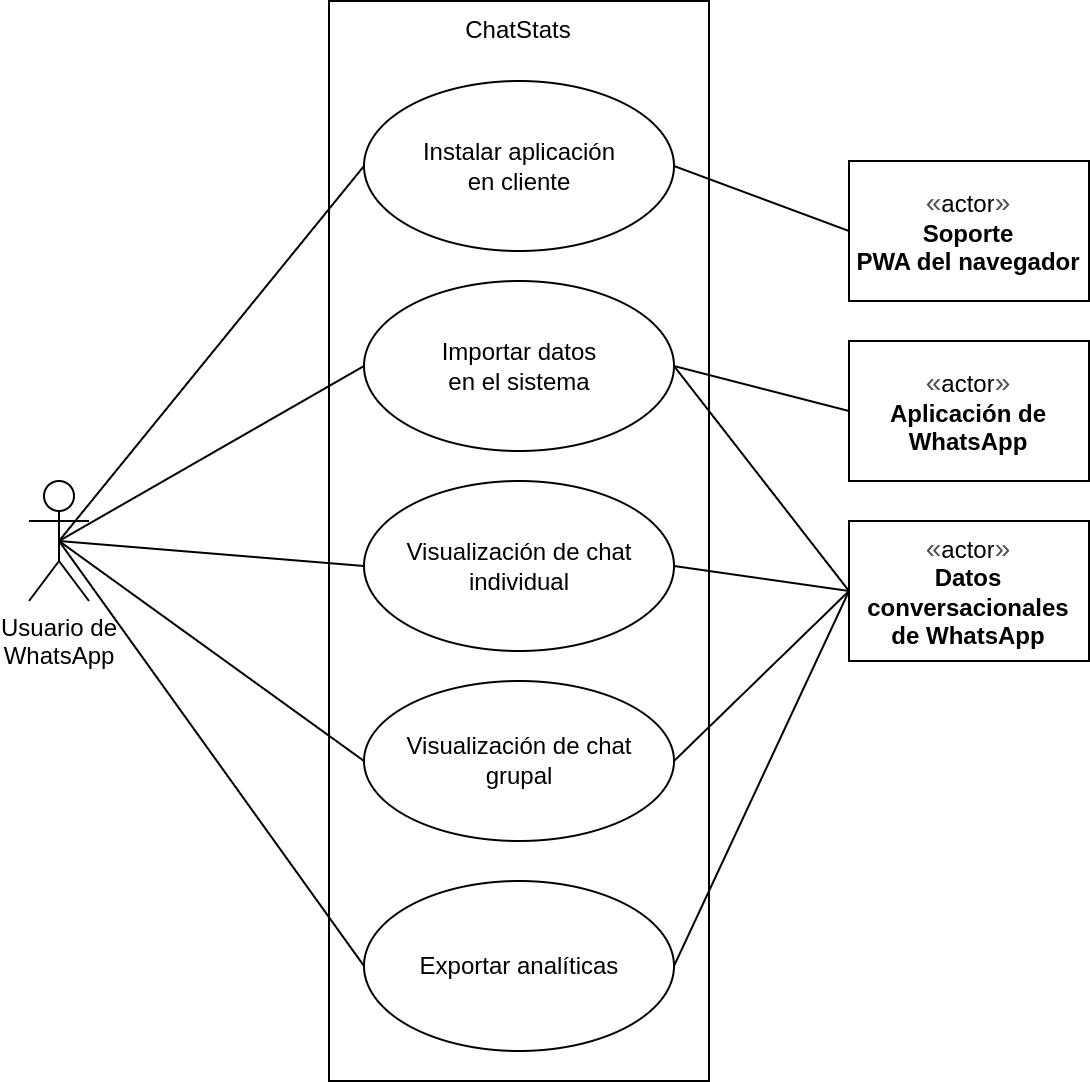
\includegraphics[width=0.8\textwidth]{img/uml.png}
	\caption{Diagrama \acrshort{uml}}
	\label{fig:chap3:uml}
\end{figure}

\begin{comment}
	Debería crear un caso de uso para chats individuales y otro para chats grupales?
	Debería diferenciar el caso de uso de PWA y web normal? (Por la integración con el SO)
	El actor es el archivo exportado y no WhatsApp.
	He cancelado el caso de uso de Telegram puesto que solo puede exportarse desde el ordenador y solo para algunos clientes.
\end{comment}

\section{Casos de uso}
\label{sec:use-cases}


\subsection{Actores del sistema}
\label{subsec:system-actors}

Usuario de WhatsApp o Telegram, datos conversacionales, aplicación de WhatsApp, aplicación de Telegram para escritorio y soporte PWA del navegador.

\paragraph{Usuario de WhatsApp o Telegram}\mbox{}\\

Se trata del usuario único en el que se centran nuestros casos de uso. Este es un usuario de WhatsApp o Telegram, ya que ChatStats es compatible con los archivos de chat exportados por estas aplicaciones.

\paragraph{Datos conversacionales}\mbox{}\\

Es el fichero de datos que nuestro sistema espera como entrada. En este caso de uso, se trata de un fichero de texto plano con todos los datos conversacionales exportados por la aplicación WhatsApp o Telegram para un chat individual o grupal, con o sin contenido multimedia.

\paragraph{Aplicación de WhatsApp}\mbox{}\\

Este actor constituye un sistema externo necesario para producir el actor anterior. Sin la aplicación de WhatsApp, ChatStats no tiene ninguna finalidad por sí solo.

\paragraph{Aplicación de Telegram para escritorio}\mbox{}\\

Este actor constituye un sistema externo necesario para producir los datos conversacionales. Sin la aplicación de Telegram para escritorio, ChatStats no tiene ninguna finalidad por sí solo.

\paragraph{Soporte \acrshort{pwa} del navegador}\mbox{}\\

Los navegadores con soporte para \acrfull{pwa} permiten instalar aplicaciones web, mejorando la integración con el sistema operativo.

\subsection{Instalar aplicación en el cliente}

\paragraph{Nombre del caso de uso} Instalar aplicación en el cliente.
\paragraph{Actores} Usuario de WhatsApp o Telegram, soporte \acrshort{pwa} del navegador.
\paragraph{Resumen} El usuario de WhatsApp o Telegram podrá, si su navegador lo soporta, instalar la aplicación de ChatStats para facilitar el acceso a la misma desde su sistema operativo y ofrecer mayor integración con el mismo.
\paragraph{Secuencia de acciones}\mbox{}\\

\begin{enumerate}
	\item El usuario accede a la página principal de ChatStats.
	\item El navegador con soporte \acrshort{pwa} le ofrece la opción de instalar la aplicación.
	\item El usuario instala la aplicación obteniendo un acceso directo en el escritorio o en el cajón de aplicaciones del navegador.
\end{enumerate}

\subsection{Importar datos en el sistema}

\paragraph{Nombre del caso de uso} Importar datos en el sistema.
\paragraph{Actores} Usuario de WhatsApp o Telegram, aplicación de WhatsApp, aplicación de Telegram para escritorio, datos conversacionales.
\paragraph{Resumen} El usuario de WhatsApp o Telegram exporta un chat de WhatsApp o Telegram, individual o grupal. Posteriormente, el usuario accede a la aplicación, selecciona e importa el archivo de datos conversacionales de WhatsApp. Finalmente, confirma su selección.
\paragraph{Secuencia de acciones}\mbox{}\\

\begin{enumerate}
	\item El usuario de WhatsApp o Telegram exporta un chat individual o grupal.
	\item El usuario accede a la aplicación.
	\item El usuario selecciona e importa el archivo de datos conversacionales exportado anteriormente.
	\item El usuario observa y confirma la selección.
\end{enumerate}

\subsection{Visualización de chat individual}

\paragraph{Nombre del caso de uso} Visualización de chat individual.
\paragraph{Actores} Usuario de WhatsApp o Telegram, datos conversacionales.
\paragraph{Resumen} El usuario puede observar, analizar e interactuar con las gráficas y estadísticas calculadas para chats individuales.
\paragraph{Secuencia de acciones}\mbox{}\\

\begin{enumerate}
	\item El usuario de WhatsApp o Telegram inicia el cálculo de estadísticas desde la aplicación.
	\item El usuario puede ver el número de mensajes enviado por ambas partes, así como el número de caracteres.
	\item El usuario puede ver la media de palabras y caracteres por mensaje.
	\item El usuario puede ver quién contesta más rápido los mensajes, así como el tiempo medio de respuesta.
	\item El usuario puede ver quién comienza normalmente las conversaciones, así como cuántas conversaciones ha comenzado cada uno.
	\item En caso de haber exportado el contenido multimedia, el usuario puede ver el número de fotos, vídeos, audios y pegatinas enviadas por ambas partes.
	\item El usuario puede ver tres distribuciones de mensajes: distribución de mensajes por mes, distribución de la media por día de la semana y distribución de la media de mensajes por hora del día.
	\item El usuario puede ver las palabras más utilizadas, así como los emoticonos.
\end{enumerate}

\paragraph{Condiciones previas} El usuario debe haber realizado anteriormente la exportación de un chat individual con o sin contenido multimedia desde la aplicación de WhatsApp o Telegram. También debe haber realizado la importación de datos en el sistema.

\subsection{Visualización de chat grupal}

\paragraph{Nombre del caso de uso} Visualización de chat grupal.
\paragraph{Actores} Usuario de WhatsApp o Telegram, datos conversacionales.
\paragraph{Resumen} El usuario puede observar, analizar e interactuar con las gráficas y estadísticas calculadas para chats grupales.
\paragraph{Secuencia de acciones}\mbox{}\\

\begin{enumerate}
	\item El usuario de WhatsApp o Telegram inicia el cálculo de estadísticas desde la aplicación.
	\item El usuario puede ver el número de mensajes enviado por cada persona, así como el número de caracteres.
	\item El usuario puede ver la media de palabras y caracteres por mensaje.
	\item El usuario puede ver quién contesta más rápido los mensajes, así como el tiempo medio de respuesta.
	\item El usuario puede ver quién comienza normalmente las conversaciones, así como cuántas conversaciones ha comenzado cada uno.
	\item En caso de haber exportado el contenido multimedia, el usuario puede ver el número de fotos, vídeos, audios y pegatinas enviadas por cada usuario.
	\item El usuario puede ver tres distribuciones de mensajes: distribución de mensajes por mes, distribución de la media por día de la semana y distribución de la media de mensajes por hora del día.
	\item El usuario puede ver las palabras más utilizadas, así como los emoticonos.
\end{enumerate}

\paragraph{Condiciones previas} El usuario debe haber realizado anteriormente la exportación de un chat grupal con o sin contenido multimedia desde la aplicación de WhatsApp o Telegram. También debe haber realizado la importación de datos en el sistema.

\subsection{Exportar analíticas}

\paragraph{Nombre del caso de uso} Exportar analíticas.
\paragraph{Actores} Usuario de WhatsApp o Telegram, datos conversacionales.
\paragraph{Resumen} El usuario puede exportar sus analíticas en un fichero, así como exportar una imagen para compartir las visualizaciones obtenidas.
\paragraph{Secuencia de acciones}\mbox{}\\

\begin{enumerate}
	\item El usuario de WhatsApp o Telegram desciende en la página de visualización.
	\item El usuario selecciona la opción de exportar o compartir.
	\item El usuario puede compartir la imagen de las visualizaciones obtenidas o guardar el archivo de los estadísticos calculados.
\end{enumerate}

\paragraph{Condiciones previas} El usuario debe haber realizado anteriormente la exportación de un chat grupal con o sin contenido multimedia desde la aplicación de WhatsApp o Telegram. También debe haber realizado la importación de datos en el sistema y el cálculo de las estadísticas para la visualización del chat.



\section{Especificación suplementaria}
\label{subsect:suplementary-specification}


\subsection{Reglas de dominio}

\begin{itemize}
	\item \textbf{Legales:} Cumplimiento de la Ley General de Protección de Datos Europea.
\end{itemize}

\begin{comment}
	No tenemos más reglas de dominio porque no tenemos requisitos o restricciones específicas a la industria o dominio de trabajo de nuestro caso de uso.
\end{comment}


\subsection{Requisitos no funcionales}

\begin{itemize}
	\item \textbf{Operación:} Interfaz de Usuario para navegador web, smartphone y tablet.
	
	\item \textbf{Seguridad:} Los datos no deben ser enviados a ningún servidor externo sin la autorización previa del usuario. Estos datos, además, no deben ser almacenados de manera temporal o permanente en ningún servidor. Todas las conexiones entre cliente y servidor deben estar cifradas con SSL.
	
	\item \textbf{Portabilidad:} La aplicación podrá ejecutarse en los navegadores: Chrome, Firefox, Edge y Safari; siendo compatible con \acrshort{pwa} en los navegadores que lo soporten.
	
	\item \textbf{Rendimiento:} El sistema debe ser capaz de analizar conversaciones de varios años sin aumentar drásticamente el tiempo de espera.
	
	\item \textbf{De implementación:} El código ha de ser libre bajo la licencia \acrfull{gplv3}.
\end{itemize}

\subsection{Restricciones}

\begin{itemize}
	\item \textbf{De interfaz:} uso de archivos \textit{txt} y \textit{zip} para importar los chats exportados desde la aplicación WhatsApp, puesto que únicamente exporta en estos dos formatos. Uso de archivos \textit{JSON} para importar los chats exportados desde la aplicación de Telegram para escritorio.
\end{itemize}











\chapter{Arquitectura}
\label{chap:architecture}


\section{Introducción}
\label{sec:introduction}

En este capítulo trataremos la fase de diseño de este proyecto, así como los detalles de implementación de la arquitectura del mismo. Primero, presentaremos una vista general del proyecto por medio de un escenario. A continuación se mostrará la arquitectura en el cliente, así como la del servidor y los servicios que la componen. Posteriormente, se detallarán los módulos que conforman la aplicación, así como las métricas que se han decidido calcular y sus motivos. Con ello tenemos la intención de facilitar al lector una vista general de la arquitectura del proyecto.

Se presenta a continuación el escenario principal de uso de ChatStats:

\begin{figure}[H]
	\centering
	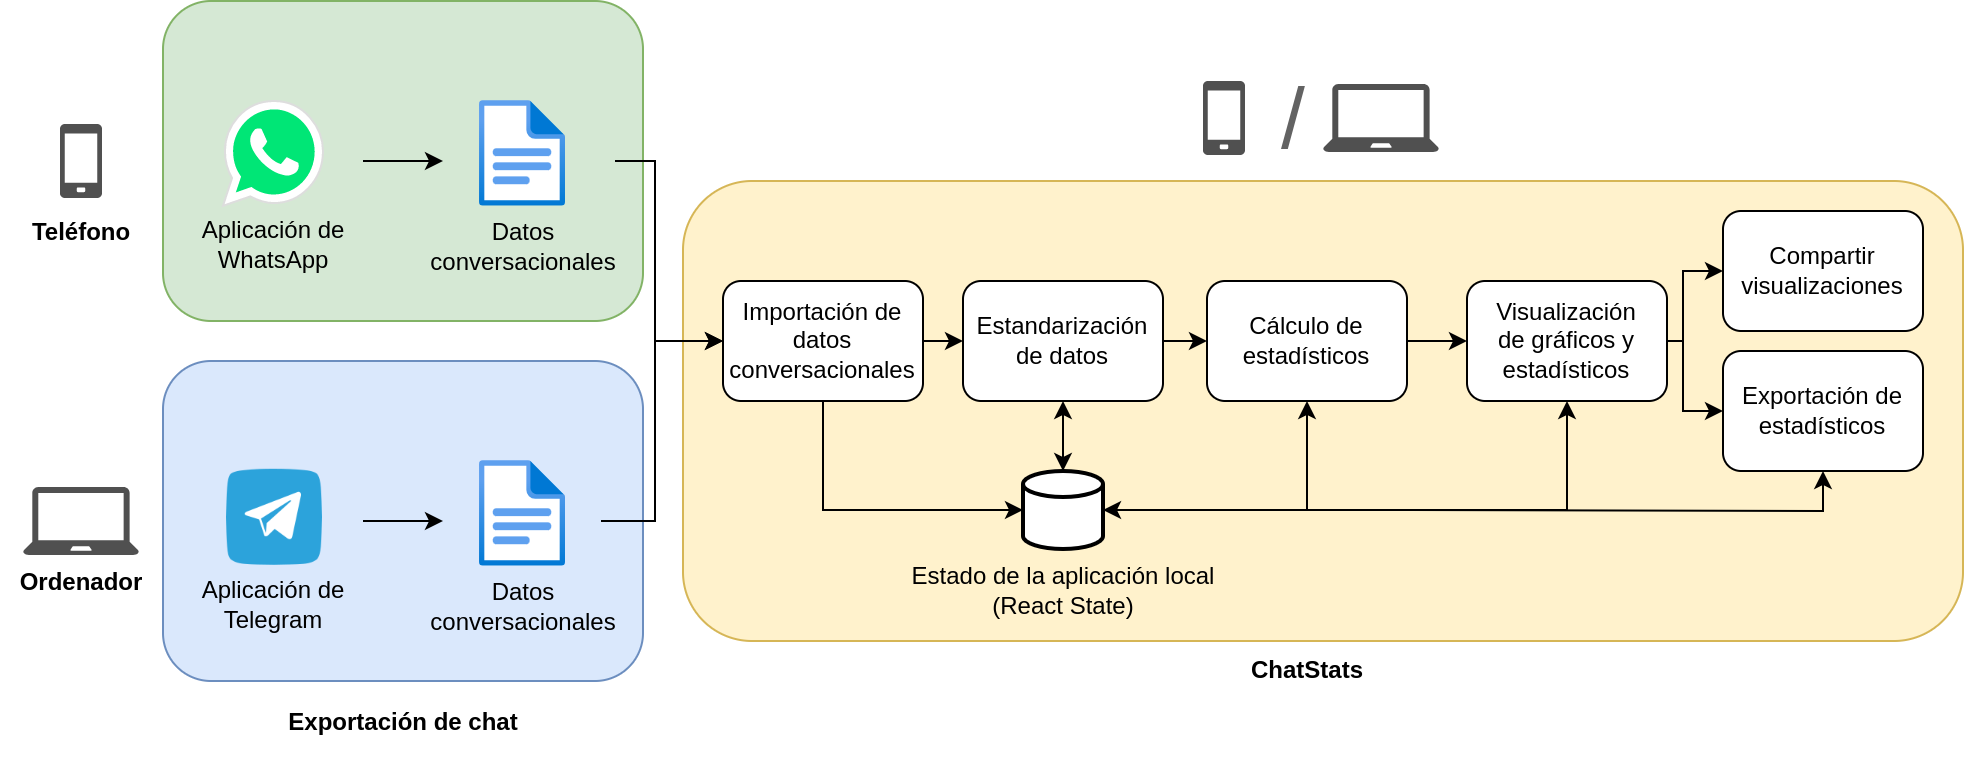
\includegraphics[width=\textwidth]{img/scenario.png}
	\caption{Escenario de ChatStats}
	\label{fig:chap4:architecture_scenario}
\end{figure}

\todi{El servidor únicamente sirve la página... ¿Debería meterlo aquí? ¿Cómo?}

Como se puede observar, el usuario debe exportar un chat desde la aplicación de WhatsApp (móvil) o Telegram para escritorio. Son estas las únicas versiones de las aplicaciones que permiten exportar las conversaciones. Con estos datos exportados, el usuario accede a ChatStats desde el navegador, ya sea en un dispositivo móvil o en un ordenador. El servidor le envía el cliente completo, por lo que no intercambia más peticiones en adelante. El usuario puede seleccionar e importar el archivo a la aplicación, que los estandariza, calcula métricas sobre la conversación y ofrece una visualización de los mismos. Finalmente, el usuario puede compartir las visualizaciones, así como exportar los datos calculados para su uso personal.


Se desarrolla toda la aplicación en \textit{JavaScript}, puesto que puede ejecutarse en todos los navegadores salvo que lo tengan deshabilitado. Otros lenguajes como \textit{PHP} o Python requieren de un servidor para realizar operaciones y que estos envíen una plantilla rellena con los resultados.



\section{Arquitectura en el cliente}

A continuación se presenta la arquitectura que podemos encontrar en un cliente cualquiera:

\begin{figure}[H]
	\centering
	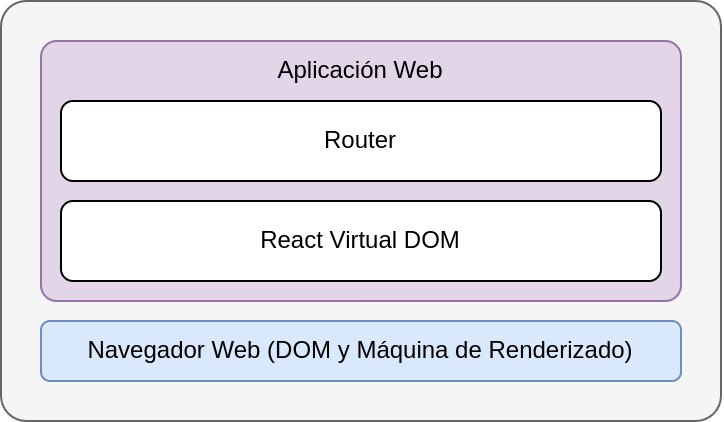
\includegraphics[width=0.6\textwidth]{img/client.png}
	\caption{Arquitectura en el cliente}
	\label{fig:chap4:architecture_client}
\end{figure}

\paragraph{Navegador.} El navegador juega un papel fundamental para el acceso y ejecución de cualquier aplicación web. Aunque no se entra en detalle en su estructura interna, sí que vamos a detallar la integración con \acrfull{pwa}. Esta integración que ofrecen algunos navegadores como los basados en Chromium, permite instalar aplicaciones web, con ventajas como:

\begin{itemize}
	\item La aplicación saldrá en el escritorio en teléfonos Android e iOS, así como en el cajón de aplicaciones del navegador.
	\item Posibilidad de acceso a notificaciones \textit{push} para el sistema (que no utilizaremos).
	\item Posibilidad de guardar en \textit{cache} el código del cliente, permitiendo su uso sin conexión a Internet.
\end{itemize}

Hay que mencionar también que Mozilla no ofrece soporte para \acrshort{pwa} en su navegador Firefox\cite{firefoxNoPWA}, aunque este puede ser habilitado mediante una extensión\cite{firefoxPWAextension}.

\paragraph{Aplicación Web.} Es la última capa, se encuentra nuestra aplicación, cuya arquitectura de procesamiento se explica en la \autoref{chap:architecture:processing}. Explicamos a continuación los componentes lógicos que se encuentran en el cliente:

\subparagraph{Router.} ChatStats es una aplicación multipágina. Esto quiere decir que cuenta con diferentes rutas web en las que se muestran diferentes páginas. La página principal consolida la ruta `\textit{/}', mientras que `\textit{/graphs}' enruta la página para la visualización de los gráficos.

\subparagraph{React Virtual DOM} El DOM virtual es un concepto de programación en el que una representación virtual de la interfaz de usuario (UI) es guardada en memoria y sincronizada con el DOM del navegador. Esto nos permite definir qué queremos en la interfaz de usuario y React conseguirá que el DOM virtual y el DOM del navegador se sincronicen.








\section{Arquitectura en el servidor}
\label{chap:architecture:server}

Se muestra a continuación una grafo de la arquitectura en el servidor, donde se muestran las capas que lo componen.

\begin{figure}[H]
	\centering
	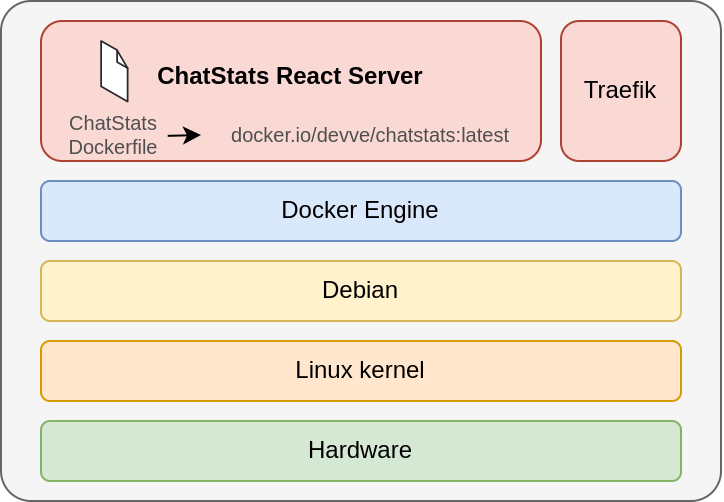
\includegraphics[width=0.6\textwidth]{img/server.png}
	\caption{Arquitectura en el servidor}
	\label{fig:chap4:architecture_server}
\end{figure}

Se ha decidido no instalar el software directamente sobre el sistema operativo, evitando problemas de dependencias y distintas versiones de las mismas para los componentes del sistema operativo. Asimismo, se evitan problemas de seguridad que puedan venir por vulnerabilidades en el código fuente y sus dependencias.

Hemos elegido virtualización ligera para ejecutar nuestro código en contenedores, por las razones que se exponen:

\begin{itemize}
	\item Se contienen las dependencias de terceros en una imagen.
	\item En caso de vulnerabilidad, solo se expone el contenedor y no el sistema completo.
	\item Los recursos se ocupan dinámicamente en función a las necesidades, al contrario que con la virtualización completa.
	\item Permite el despliegue en cualquier sistema operativo compatible con Linux, salvo arquitecturas ARM (que no es frecuente en servidores).
\end{itemize}

\paragraph{ChatStats React Server.} Se trata del servidor de React que sirve el contenido. Tras construir la versión de producción con el código fuente, este contenedor sirve el contenido estático final, que enviará al cliente completamente cuando este solicite la aplicación web. Se ha implementado por medio de un fichero Dockerfile, que parte de una imagen de \textit{NodeJS}, instala las dependencias y sirve el contenido. Con esta secuencia de instrucciones, se ha creado una imagen para uso en contenedores Docker, que puede encontrarse públicamente en el repositorio de imágenes DockerHub.

\paragraph{Traefik} Se ha decidido usar Traefik como \textit{proxy} inverso, que se sitúa frente al servidor de ChatStats para redirigir las peticiones realizadas a su contenedor correspondiente en el puerto adecuado.

Además, Traefik gestiona los certificados \acrshort{ssl} haciendo uso de \textit{Let's Encrypt}: autoridad sin ánimo de lucro que provee certificados para la capa \acrshort{tls} sin coste alguno.








\section{Arquitectura de la aplicación}
\label{chap:architecture:processing}


Con el objetivo de mantener la privacidad de los datos del usuario, se ha planteado una arquitectura centrada en el cliente, donde el servidor únicamente envía la totalidad de la aplicación al cliente en la primera petición. Esto supone un mayor coste computacional en el cliente para realizar todas las operaciones necesarias, por lo que la eficiencia del código es necesaria. Además, esta arquitectura se puede extender, en un futuro, ofreciendo analíticas adicionales si el usuario opta por enviar información al servidor para su procesamiento. Este caso de extensión se detallará más adelante.

A continuación se muestra la arquitectura de la lógica de negocio en la aplicación:

\begin{figure}[H]
	\centering
	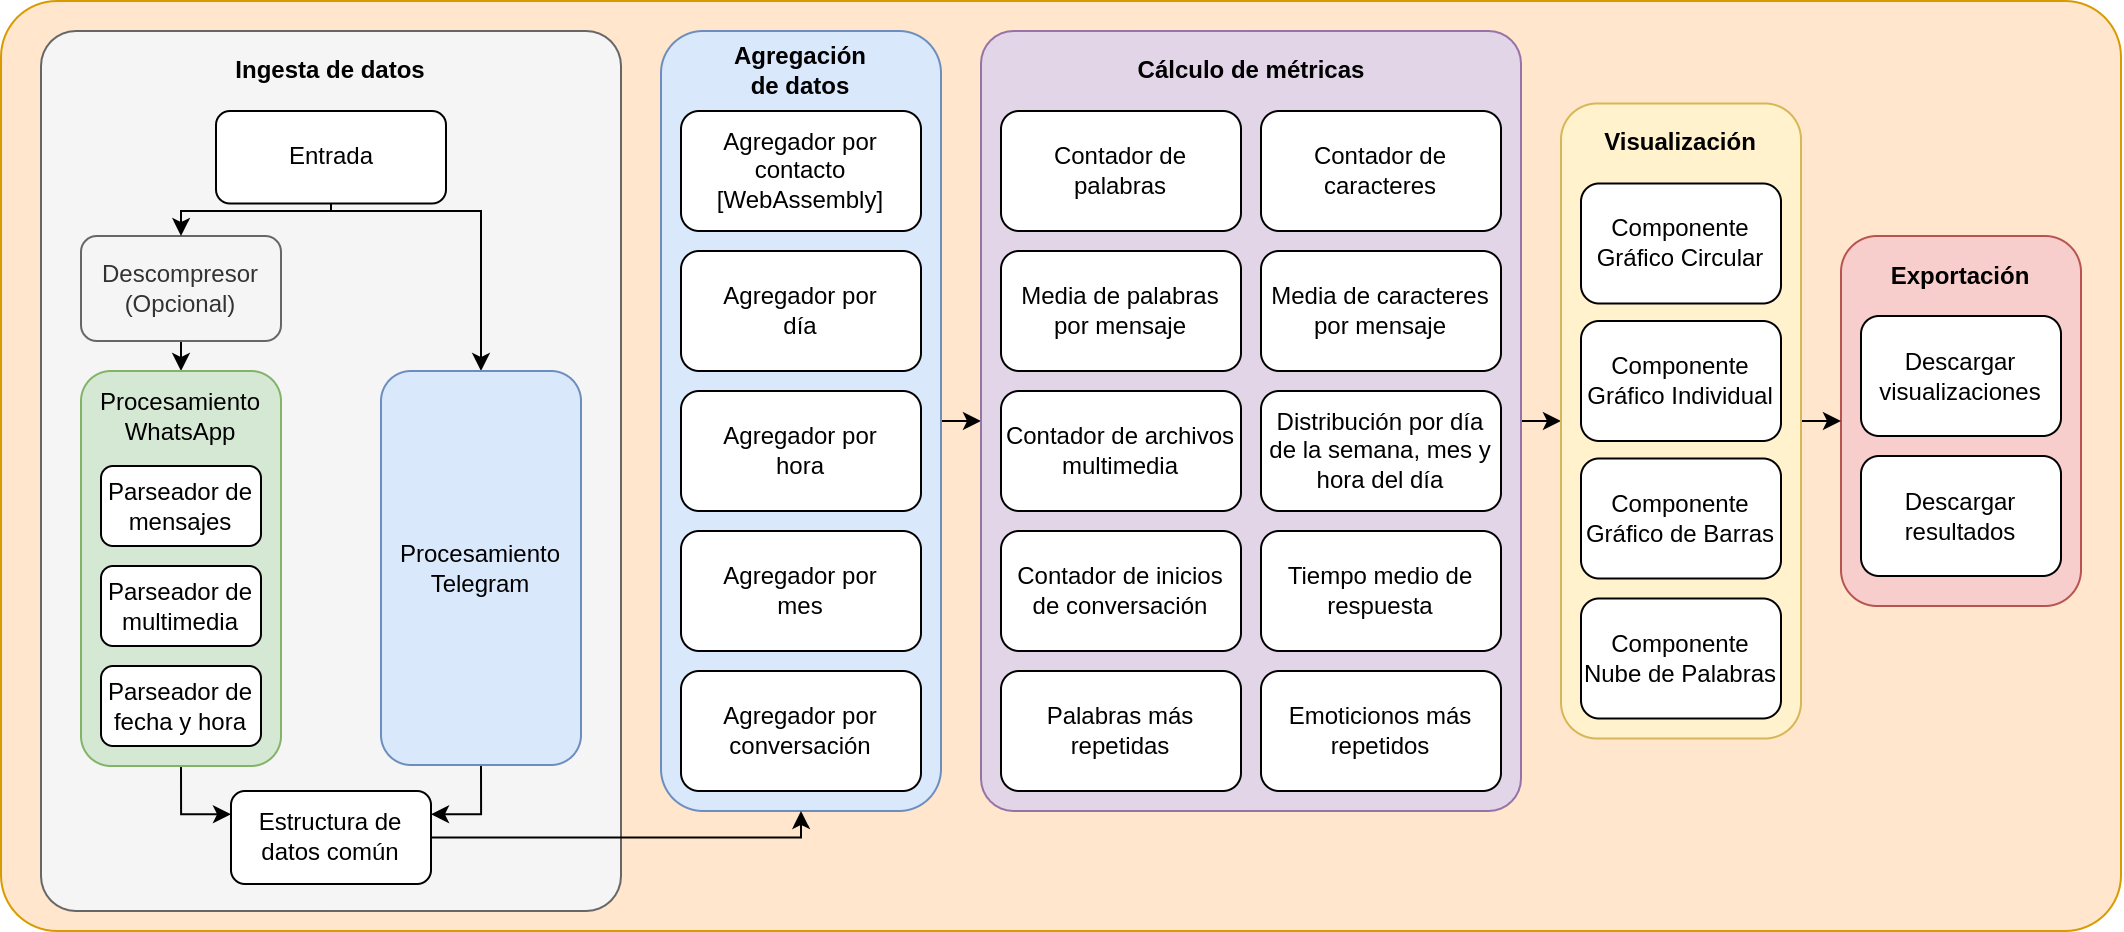
\includegraphics[width=\textwidth]{img/architecture_processing.png}
	\caption{Arquitectura de la aplicación}
	\label{fig:chap4:architecture_processing}
\end{figure}

\subsection{Importador}

El módulo importador se encarga de leer el fichero de entrada. Dicho fichero puede estar en tres formatos diferentes:

\begin{itemize}
	\item \textit{txt} si se trata de un chat exportado de WhatsApp en un dispositivo Android.
	\item \textit{zip} si se trata de un chat exportado de WhatsApp desde un dispositivo iOS.
	\item \textit{\acrshort{json}} si se trata de un chat exportado de Telegram desde la aplicación para escritorio.
\end{itemize}

Aunque Telegram también soporta la exportación de conversaciones en \textit{HTML}, ChatStats no soporta este formato, puesto que está diseñado para la visualización y no para el tratamiento y procesado del mismo.

En caso de exportar el chat con contenido multimedia, ChatStats únicamente espera el fichero de texto plano (ya sea directamente o dentro de un archivo comprimido), puesto que este se encuentran todos los datos necesarios para el análisis del contenido multimedia. Es por ello que todo el contenido multimedia recibido se descarta.

\subsubsection{Entrada}

Este submódulo se encarga de cargar el fichero seleccionado por el usuario, que el navegador ofrece desde una ruta falsa y protegida para que la aplicación no pueda acceder a todos los archivos del dispositivo. En caso de tratarse de un fichero de texto plano, este módulo abre el archivo como una cadena de caracteres. En caso de tratarse de un fichero comprimido, se lo envía al módulo ``Descompresor'' esperando un archivo de texto plano como salida. Por último, en caso de tratarse de cualquier otro tipo de fichero, el módulo alerta al usuario de que el archivo de entrada no es válido.

Este submódulo hace uso de una instancia de \textit{FileReader}; clase que ofrecen los navegadores, permitiendo abrir el fichero como secuencia de caracteres.

\subsubsection{Descompresor (Opcional)}

Este submódulo se encarga de la descompresión de ficheros \textit{zip}, que descomprime bajo petición del módulo anterior. Finalmente, el módulo devuelve un fichero llamado \textit{\_chat.txt}, que, como se ha comentado anteriormente, contiene toda la información necesaria para el análisis (con o sin multimedia).

El descompresor hace uso de la librería \textit{jszip} para la descompresión del fichero. La lógica añadida a esta aplicación nos permite encontrar el fichero de texto plano dentro del fichero comprimido y devolver el mismo al módulo de ``Entrada''.

\subsection{Parseador}

El objetivo de este módulo es estandarizar los datos de entrada con la finalidad de poder utilizar los mismos módulos para cualquier archivo de entrada.

Mientras que Telegram ofrece los datos en formato \acrshort{json}, facilitando así la operabilidad de los mismos; WhatsApp no ofrece una estructura de datos ni consistencia entre distintas versiones de su aplicación.

Se expone a continuación un breve ejemplo del formato utilizado por Telegram:

\begin{lstlisting}[language=JavaScript]
	{
		"name": "group_or_contact_name",
		"type": "private_group_or_private_chat",
		"id": 00000000,
		"messages": [
		...
		{
			"id": 11111,
			"type": "message_service",
			"date": "2019-04-02T20:53:14",
			"date_unixtime": "1554231194",
			"from": "Alice",
			"from_id": "contact_user_id",
			"text": "actual_body_message",
			"text_entities": [
			{
				"type": "plain_link_or_document",
				"text": "actual_body_message"
			}
			]
		},
		{
			"id": 22222,
			"type": "message",
			"date": "2019-05-29T23:46:00",
			"date_unixtime": "1559166360",
			"from": "Bob",
			"from_id": "contact_user_id",
			"reply_to_message_id": 59386,
			"file": "stickers/sticker.webp",
			"thumbnail": "stickers/sticker.webp_thumb.jpg",
			"media_type": "sticker",
			"sticker_emoji": "actual_unicode_emoji",
			"width": 512,
			"height": 341,
			"text": "",
			"text_entities": []
		}, ...
		]
	}
\end{lstlisting}

También se muestra un mensaje en el formato de exportación de WhatsApp en los dispositivos Android:

\begin{lstlisting}
	17/07/2022, 01:28 - Alice: Este es un mensaje de prueba
\end{lstlisting}

Así como un mensaje exportado desde WhatsApp por un dispositivo iOS:

\begin{lstlisting}
	[29/12/22, 0:14:55] Bob: Te escribo desde mi iPhone.
\end{lstlisting}

Podemos observar que, en el caso de WhatsApp, ambos mensajes se componen de la fecha, la hora, el nombre del contacto y el propio cuerpo del mensaje, aunque con distinto formato. Dicha información está disponible también en los mensajes de Telegram.

\subsubsection{Parseador de mensajes}

El objetivo del submódulo es convertir la cadena de caracteres de entrada en mensajes con el siguiente formato \acrshort{json}:

\begin{lstlisting}[language=JavaScript]
	{
		date: new Date("2022-10-17T10:37:00"),
		from: "Juan Pedro",
		text: "IMG-20221020-WA0013.jpg",
		type: "message",
		media_type: "image"
	}
\end{lstlisting}

Hemos decidido esta estructura ya que se trata de toda la información que podemos obtener de mensajes de WhatsApp. Además, es compatible con la estructura ya propuesta por Telegram. Podemos decir entonces que es un máximo común denominador de la información disponible en ambos casos. Serán estos los objetos que se utilizarán más adelante para calcular las estadísticas y las estructuras de datos de visualización.

Es por ello que analizamos ambos casos por separado:

\paragraph{Telegram} En caso de tratar un fichero en formato \acrshort{json}, utiliza la librería \textit{JSON} nativa para \textit{JavaScript}, parseando todo el contenido del módulo ``Importador'' y eliminando los datos del objeto original que no se van a utilizar. Posteriormente, llama al módulo ``Parseador de fecha y hora'' que se describe más adelante.

\paragraph{WhatsApp} En caso de tratar con un fichero de WhatsApp, se llega a la siguiente expresión regular que nos permite separar las partes del mensaje, tanto para Android como para iOS.

\begin{lstlisting}
	/\[*(\d{1,2}\/\d{1,2}\/\d{2,4}),\s(\d{1,2}:\d{2}:*\d*)\]*\s(?:-\s)*(.*?):{1}\s(.*?)(?=\s\[*\d{1,2}\/\d{1,2}\/\d{2,4}|$)/gum
\end{lstlisting}

Los grupos de captura que lo componen se describen en detalle en el \autoref{chap:regex}.


\subsubsection{Parseador de fecha y hora}

Este submódulo tiene como entrada la fecha y la hora. Devuelve un objeto de tipo \textit{Date}, nativo de JavaScript. Esto nos permite realizar operaciones de tiempo con facilidad en otros módulos.

Este submódulo utiliza la librería \textit{momentjs} para parsear los posibles distintos formatos de fecha que utilizan Telegram y WhatsApp en sus cadenas de caracteres. Además, considera el \textit{locale} del cliente, invirtiendo mes y día para el caso \textit{en\_US}.

La salida de este submódulo se utiliza en la clave \textit{``date''} del objeto mensaje del submódulo anterior.

\subsubsection{Parser de archivos multimedia}

Este submódulo se ejecuta únicamente para chats exportados por WhatsApp. El objetivo de este submódulo es escribir el tipo de contenido en la clave \textit{``media\_type''} del objeto mensaje expuesto anteriormente.

Existen dos opciones para exportar un chat: con contenido multimedia o sin él.

\paragraph{Para contenido multimedia}\mbox{}\\

En el fichero de texto plano con contenido multimedia, observaremos que el cuerpo incluye el nombre del fichero que se ha exportado con la extensión del formato del mismo. Por ello, categorizamos como \textit{voice\_message}, \textit{video\_file}, \textit{sticker} o \textit{image} en función a la extensión; \textit{.opus}, \textit{.mp4}, \textit{.webp} o \textit{.jpg}, respectivamente. Usamos estos valores puesto que son los que Telegram utiliza para su formato de mensajes.

Se indican a continuación mensajes de ejemplo para cada tipo de archivo adjunto, únicamente para Android:

\begin{lstlisting}
	17/10/2022, 21:11 - Juan Pedro: PTT-20221017-WA0078.opus (file attached)
	20/10/2022, 10:37 - Juan Pedro: IMG-20221020-WA0013.jpg (file attached)
	14/11/2022, 18:58 - Juan Pedro: VID-20221114-WA0039.mp4 (file attached)
	24/11/2022, 19:13 - Jaime Conde: STK-20220717-WA0090.webp (file attached)
\end{lstlisting}

\paragraph{Sin contenido multimedia}\mbox{}\\

Para el segundo caso, cada vez que un mensaje sea contenido multimedia, aparecerá \textit{\textless Media omitted \textgreater} (multimedia omitido). Estos pueden ser fotos, vídeos, música, notas de voz o documentos. Se definirán como \textit{undefined} o indefinidos, ignorándose en las visualizaciones y módulos posteriores.

\begin{lstlisting}
	17/07/2022, 01:33 - Juan Pedro: <Media omitted>
\end{lstlisting}

\subsection{Agregador}

Los mensajes se encuentran segregados en una lista, por lo que a continuación, el módulo de agregador se encargará de agregar los mensajes en diferentes grupos. En el código los hemos llamado polarizadores. Se describen los distintos submódulos a continuación:

\subsubsection{Agregador por contacto}

\textit{ChatStats} se encarga de calcular las estadísticas de cada contacto para visualizarlas y mostrarlas en comparación con el resto de contactos. Hablamos de numerosos contactos, puesto que es compatible con chats individuales y grupales.

El resultado de este submódulo será un objeto \acrshort{json} con una clave por cada contacto (su nombre), que contendrá un array de los mensajes enviados por este. Se indica un ejemplo:

\begin{lstlisting}[language=JavaScript]
	{
		"Jaime": [...messagesByJaime],
		"Juan Pedro": [...messagesByJuanPedro],
		...
	}
\end{lstlisting}

donde los array de mensajes contienen objetos definidos en el \textit{Parser de mensajes}.

\subsubsection{Agregador por día}

Este agregador toma como entrada la salida del submódulo anterior: los mensajes agregados por contacto. Con ello se procede a agregarlos, además, por día de la semana: de lunes a domingo. Se usará el nombre del día de la semana como clave anidada.

El resultado son objetos con la siguiente estructura:

\begin{lstlisting}[language=JavaScript]
	{
		"Jaime": {
			"monday": [...messagesByJaimeOnMonday],
			"tuesday": [...messagesByJaimeOnTuesday],
			...,
			"sunday": [...messagesByJaimeOnSunday]
			},
		"Juan Pedro": {
			"monday": [...messagesByJuanPedroOnMonday],
			"tuesday": [...messagesByJuanPedroOnTuesday],
			...,
			"sunday": [...messagesByJuanPedroOnSunday]
		},
		...
	}
\end{lstlisting}

El objetivo de esta estructura de datos es visualizar la distribución de los mensajes a lo largo de la semana, en media.

\begin{comment}
	Se deja para futuras líneas un gráfico en el que se pueda elegir el año a analizar, o un scroll vertical por años.
\end{comment}

\subsubsection{Agregador por hora}

Este agregador toma también como entrada los mensajes agregados por contacto. Con ello se procede a agregarlos, además, por hora del día, usando la hora en formato 24 horas como clave anidada de agregación: de 00 a 23 horas.

El resultado son objetos con la siguiente estructura:

\begin{lstlisting}[language=JavaScript]
	{
		"Jaime": {
			"00": [...messagesByJaimeAt00],
			"01": [...messagesByJaimeAt01],
			...,
			"23": [...messagesByJaimeAt23]
		},
		"Juan Pedro": {
			"00": [...messagesByJuanPedroAt00],
			"01": [...messagesByJuanPedroAt01],
			...,
			"23": [...messagesByJuanPedroAt23]
		},
		...
	}
\end{lstlisting}

El objetivo de esta estructura de datos es visualizar la distribución de los mensajes a lo largo del día, en media.

\subsubsection{Agregador por mes}

Este agregador toma también como entrada los mensajes agregados por contacto. Con ello se procede a agregarlos, además, por MM/YYYY, por lo que deja de tratarse de un agregador acotado: pueden haber tantas claves anidadas como meses se haya hablado.

El resultado son objetos con la siguiente estructura:

\begin{lstlisting}[language=JavaScript]
	{
		"Jaime": {
			"10/2022": [...messagesByJaimeOnOctober2022],
			"11/2022": [...messagesByJaimeOnNovember2022],
			...
		},
		"Juan Pedro": {
			"10/2022": [...messagesByJuanPedroOnOctober2022],
			"11/2022": [...messagesByJuanPedroOnNovember2022],
			...
		},
		...
	}
\end{lstlisting}

El objetivo de esta estructura de datos es visualizar la distribución de los mensajes a lo largo del tiempo, con una agregación mensual.

\subsubsection{Agregador por conversación}

Este submódulo analiza las diferencias de tiempos entre los mensajes, categorizándolos como inicio de conversación si son el primer mensaje en las últimas 5 horas, o como respuesta si se trata de un intervalo de tiempo menor. Esto nos permitirá calcular cuántas conversaciones ha iniciado cada contacto, así como el tiempo de respuesta medio de cada uno; módulos que se verán más adelante.

Aunque un sesgo temporal no es una solución perfecta, acierta gran parte de las veces sin necesitar gran capacidad de cómputo.

\subsection{Visualizador}

Este módulo prepara los datos para ser representados por la librería de visualización elegida: \textit{ChartJS}.  Esta librería ha sido elegida por su alta actividad de contribuciones al proyecto, que es libre y cuenta con 12 mil estrellas en GitHub. Además, permite alta extensibilidad mediante plugins, de los que hacemos uso, por ejemplo, para mostrar las etiquetas de los datos.

Cada módulo aquí desarrollado realiza el cálculo de una métrica, cuyo resultado pasa por una función que adapta el contenido a la estructura solicitada por \textit{ChartJS}. \textit{ChartJS} nos permite un único formato de entrada para los datos, permitiéndonos elegir el tipo de gráfico de forma independiente a dichos datos. Esta arquitectura nos permite añadir más módulos posteriormente; realizando el cálculo de la métrica a mostrar y pasándolo por la función que estandariza los datos para \textit{ChartJS}.

Todos los submódulos que utilizan \textit{ChartJS} adaptan el tamaño del gráfico al número de contactos que hay en el grupo de forma \textit{responsive}. También permiten la interacción con el mismo, pudiendo eliminar contactos de la representación haciendo click sobre el nombre de los mismos en la leyenda.

Además, también se procesan datos para otras librerías de visualización, como \textit{react-wordcloud}, para las nubes de palabras o \textit{word clouds} y nubes de emoticonos.

\subsubsection{Contador de mensajes}

Este submódulo cuenta el número de mensajes enviado por cada contacto. Para chats grupales, usa la librería \textit{ChartJS}, mientras que para chat individuales, únicamente se exponen los números de ambas partes directamente.

\begin{figure}[H]
	\centering
	\subfloat[\centering Chat individual]{{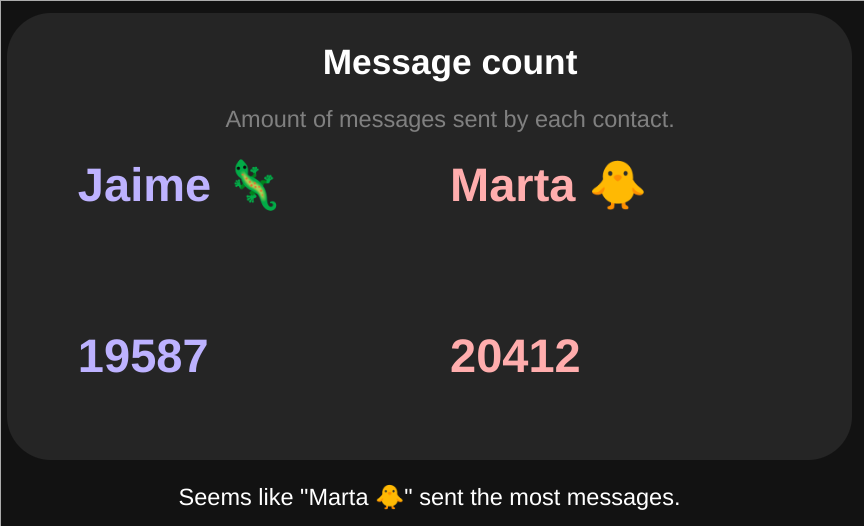
\includegraphics[width=6cm]{img/message_count_individual.png} }}
	\qquad
	\subfloat[\centering Chat grupal]{{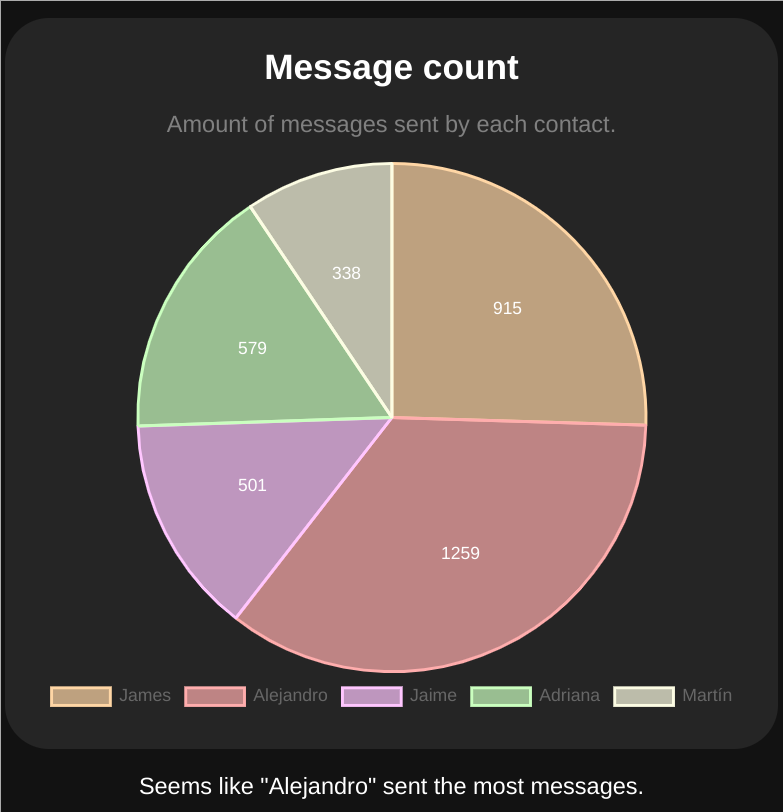
\includegraphics[width=6cm]{img/message_count.png} }}
	\caption{Contador de mensajes}
	\label{fig:chap4:message_count}
\end{figure}

Se ha optado por calcular esta métrica puesto que puede ayudar a observar diferencias drásticas en la cantidad de texto que aporta cada contacto.

\subsubsection{Contador de palabras}

Este submódulo cuenta las palabras que hay en los mensajes de cada contacto y calcula la suma total de las mismas, obteniendo el número de palabras totales enviadas por cada contacto. Para chats grupales, usa la librería \textit{ChartJS}, mientras que para chat individuales, únicamente se exponen los números de ambas partes directamente.

\begin{figure}[H]
	\centering
	\subfloat[\centering Chat individual]{{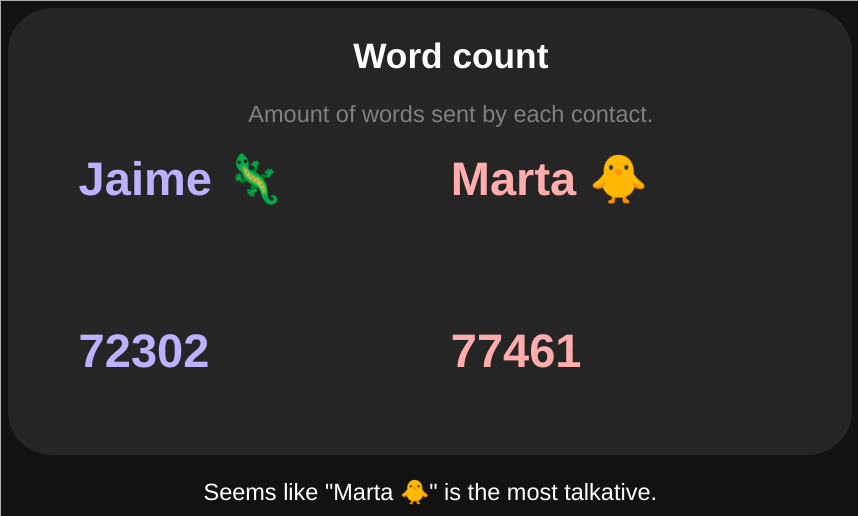
\includegraphics[width=6cm]{img/word_count_individual.png} }}
	\qquad
	\subfloat[\centering Chat grupal]{{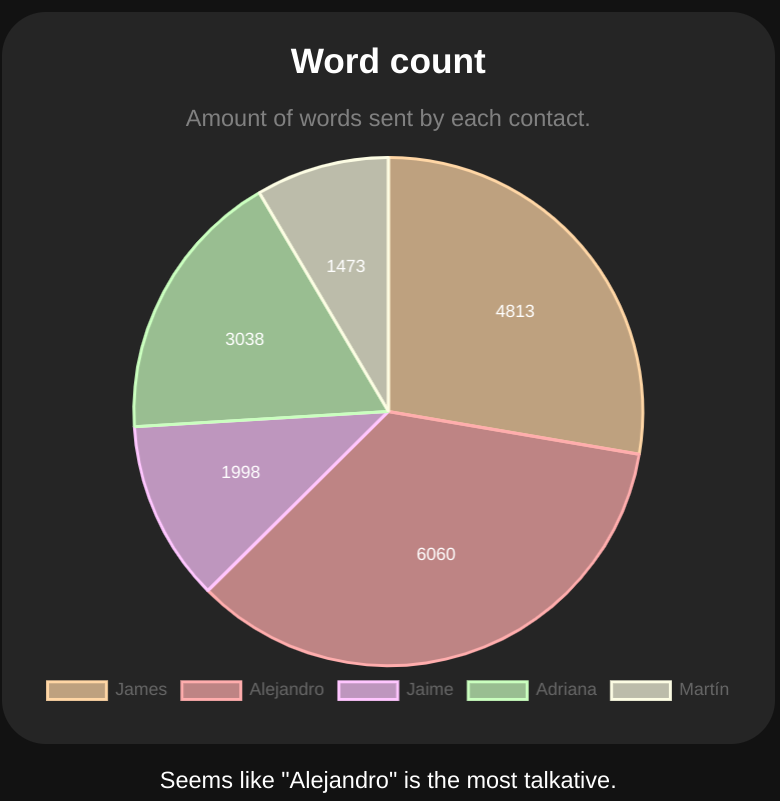
\includegraphics[width=6cm]{img/word_count.png} }}
	\caption{Contador de palabras}
	\label{fig:chap4:word_count}
\end{figure}

\subsubsection{Contador de caracteres}

Este submódulo cuenta los caracteres que hay en los mensajes de cada contacto y calcula la suma total de los mismos, obteniendo el número de caracteres totales enviados por cada contacto. Aunque suele indicar resultados similares al módulo anterior, en algunas ocasiones es distinto, por lo que se ha decidido incluir también.

\begin{figure}[H]
	\centering
	\subfloat[\centering Chat individual]{{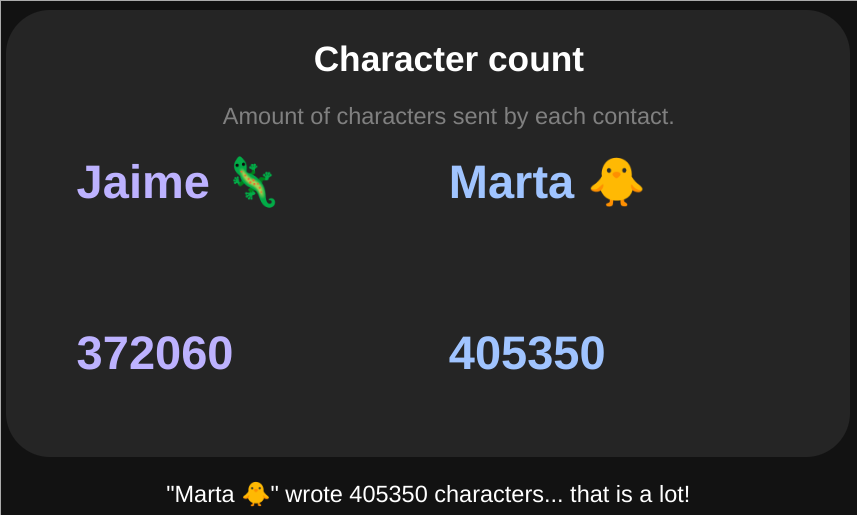
\includegraphics[width=6cm]{img/char_count_individual.png} }}
	\qquad
	\subfloat[\centering Chat grupal]{{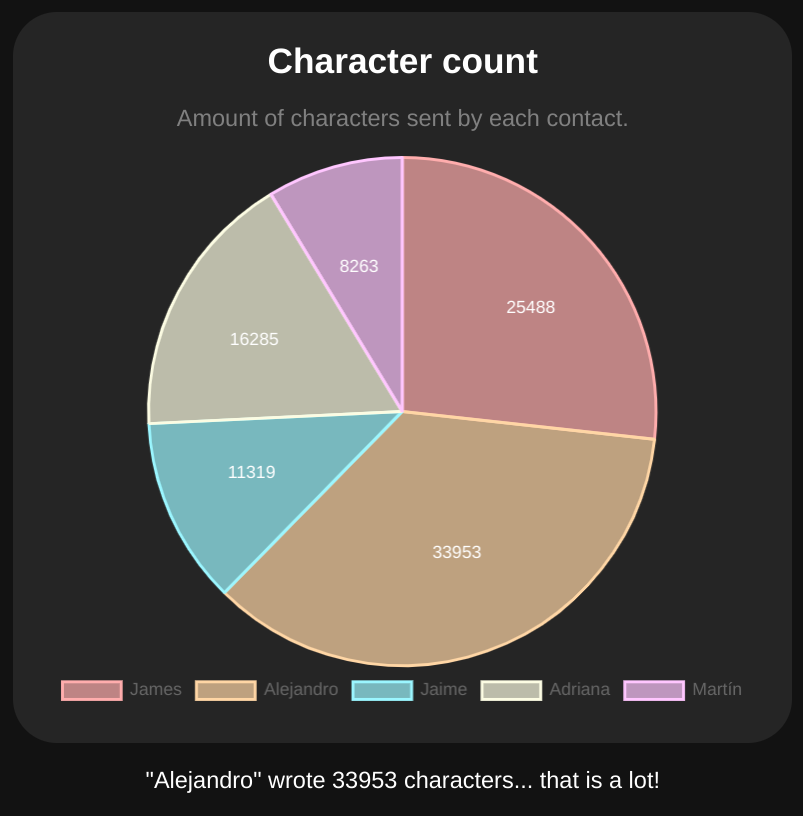
\includegraphics[width=6cm]{img/char_count.png} }}
	\caption{Contador de caracteres}
	\label{fig:chap4:char_count}
\end{figure}

De nuevo, para chats grupales, usa la librería \textit{ChartJS}, mientras que para chat individuales, únicamente se exponen los números de ambas partes directamente.

\subsubsection{Media de palabras por mensaje}

Este submódulo calcula y muestra el número medio de palabras por mensaje para cada contacto. Esta métrica puede ayudar, junto con el número de mensajes totales, a saber si un contacto tiende a mandar más mensajes con menor número de palabras, o menos mensajes con más palabras.

\begin{figure}[H]
	\centering
	\subfloat[\centering Chat individual]{{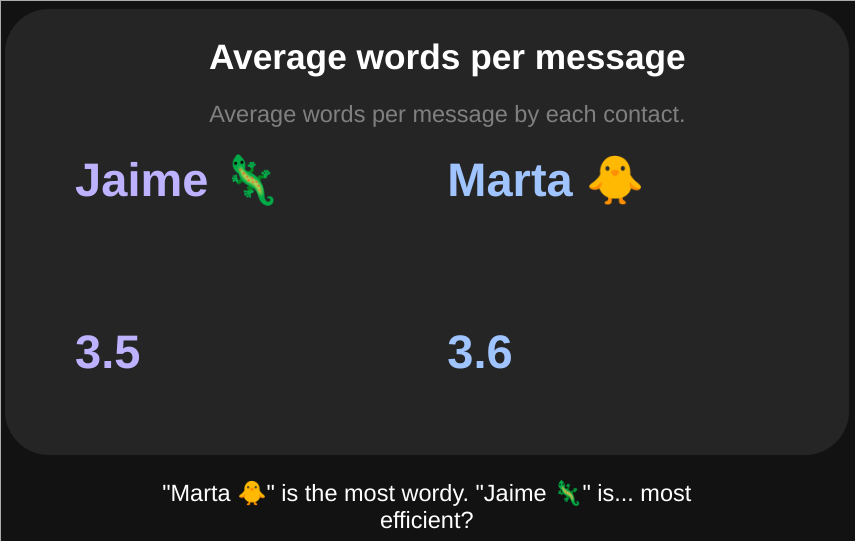
\includegraphics[width=6cm]{img/word_avg_individual.png} }}
	\qquad
	\subfloat[\centering Chat grupal]{{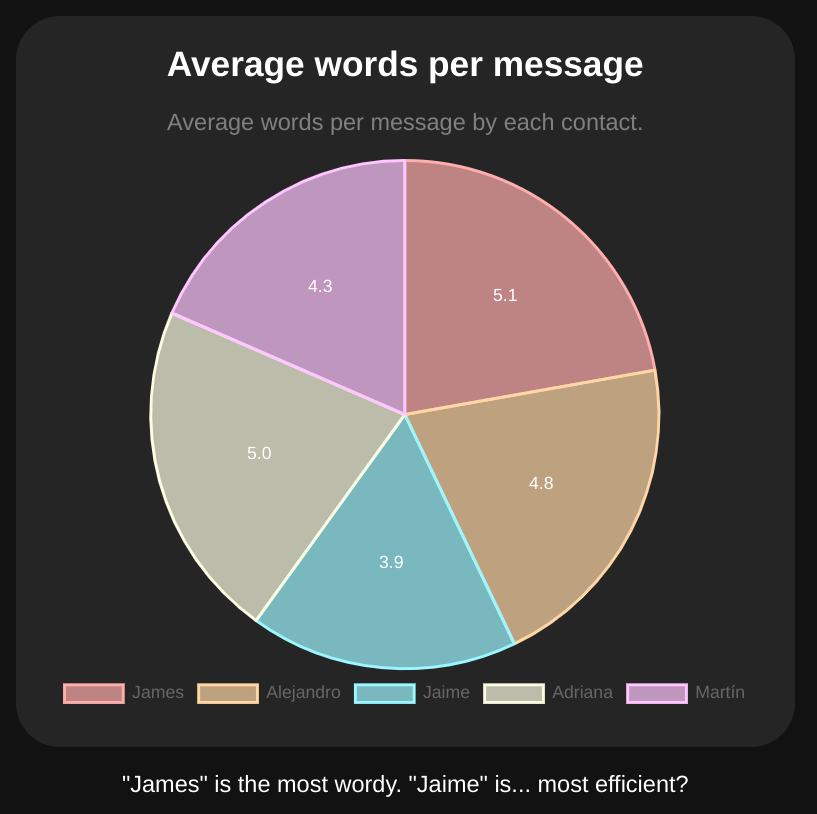
\includegraphics[width=6cm]{img/word_avg.png} }}
	\caption{Media de palabras por mensaje}
	\label{fig:chap4:word_avg}
\end{figure}

\subsubsection{Media de caracteres por mensaje}

Este submódulo calcula y muestra el número medio de caracteres por mensaje para cada contacto. Aunque suele indicar resultados similares al módulo anterior, en algunas ocasiones puede resaltar personas que tienden a usar palabras más largas.

\begin{figure}[H]
	\centering
	\subfloat[\centering Chat individual]{{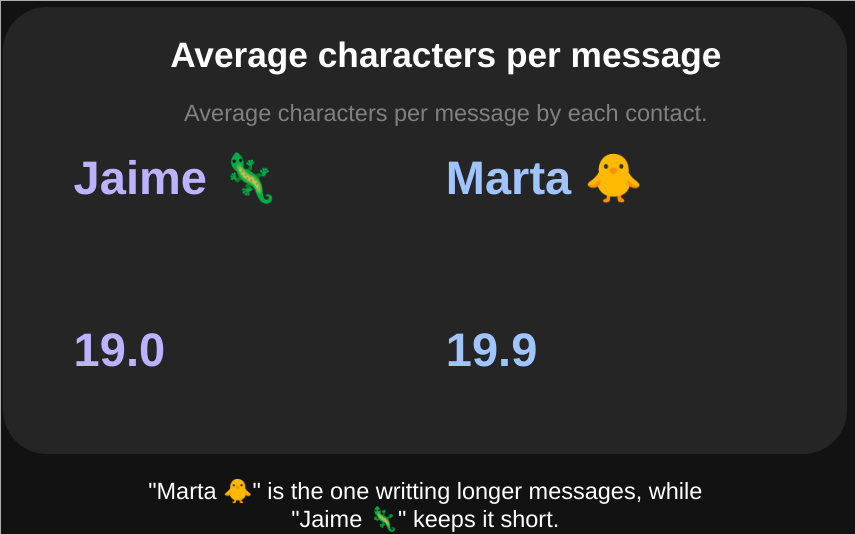
\includegraphics[width=6cm]{img/char_avg_individual.png} }}
	\qquad
	\subfloat[\centering Chat grupal]{{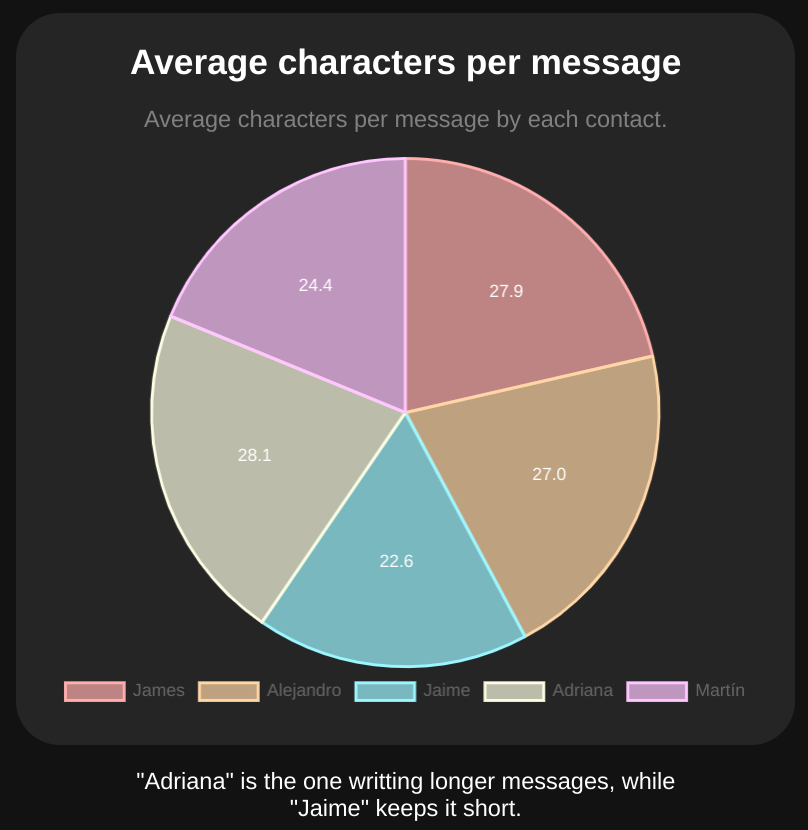
\includegraphics[width=6cm]{img/char_avg.png} }}
	\caption{Media de caracteres por mensaje}
	\label{fig:chap4:char_avg}
\end{figure}

\subsubsection{Número de conversaciones iniciadas}

Este submódulo calcula el número de veces que cada contacto ha iniciado la conversación, con los criterios y datos obtenidos del módulo ``Agregador por conversación''. Se ha decidido calcular esta métrica puesto que es una buena forma de medir la iniciativa de una persona, así como su interés en el grupo o persona individual.

\begin{figure}[H]
	\centering
	\subfloat[\centering Chat individual]{{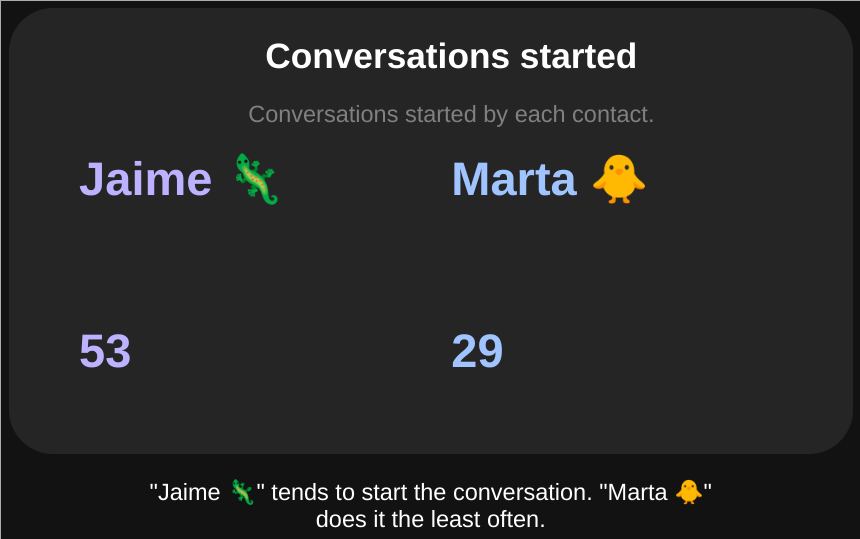
\includegraphics[width=6cm]{img/conversations_started_individual.png} }}
	\qquad
	\subfloat[\centering Chat grupal]{{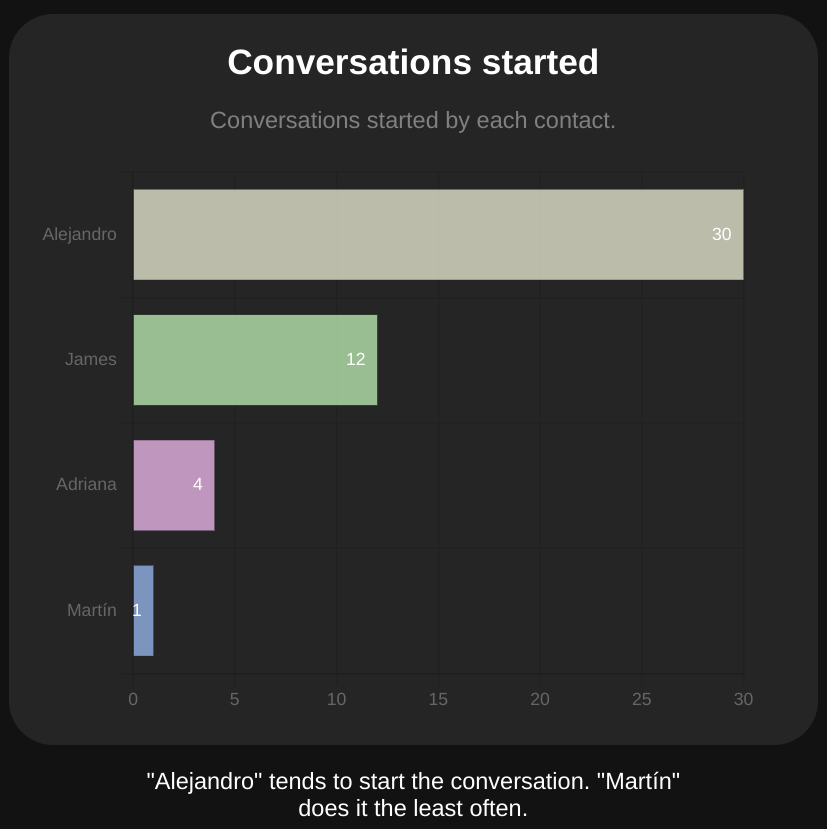
\includegraphics[width=6cm]{img/conversations_started.png} }}
	\caption{Conversaciones iniciadas por cada contacto}
	\label{fig:chap4:conversations_started}
\end{figure}

En este ejemplo, podemos ver cómo Alejandro, el presidente de la asociación, suele tomar la iniciativa y comenzar las conversaciones.


\subsubsection{Velocidad media de respuesta}

Este submódulo calcula la velocidad media de respuesta de cada contacto, con los criterios y datos obtenidos del módulo ``Agregador por conversación''. Se ha decidido calcular esta métrica puesto que es una buena forma de medir la atención a la aplicación de mensajería instantánea, así como la importancia que le da al grupo.

\begin{figure}[H]
	\centering
	\subfloat[\centering Chat individual]{{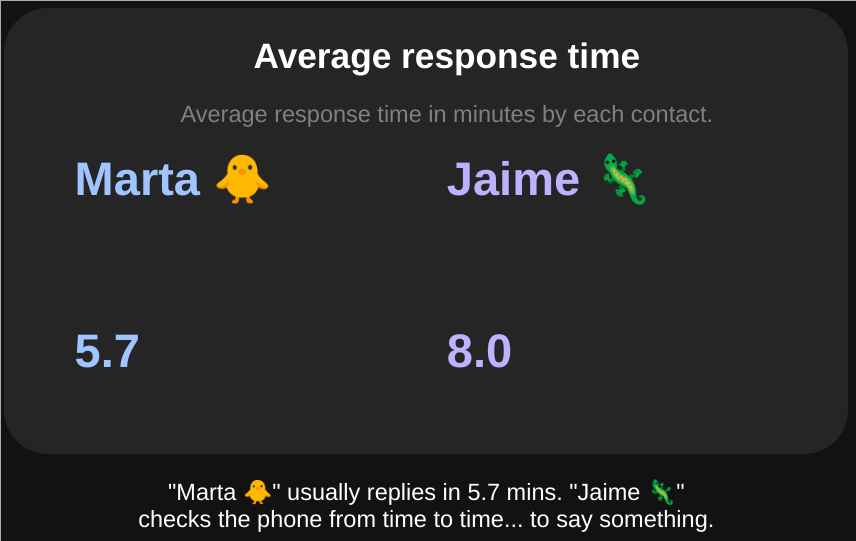
\includegraphics[width=6cm]{img/avg_response_time_individual.png} }}
	\qquad
	\subfloat[\centering Chat grupal]{{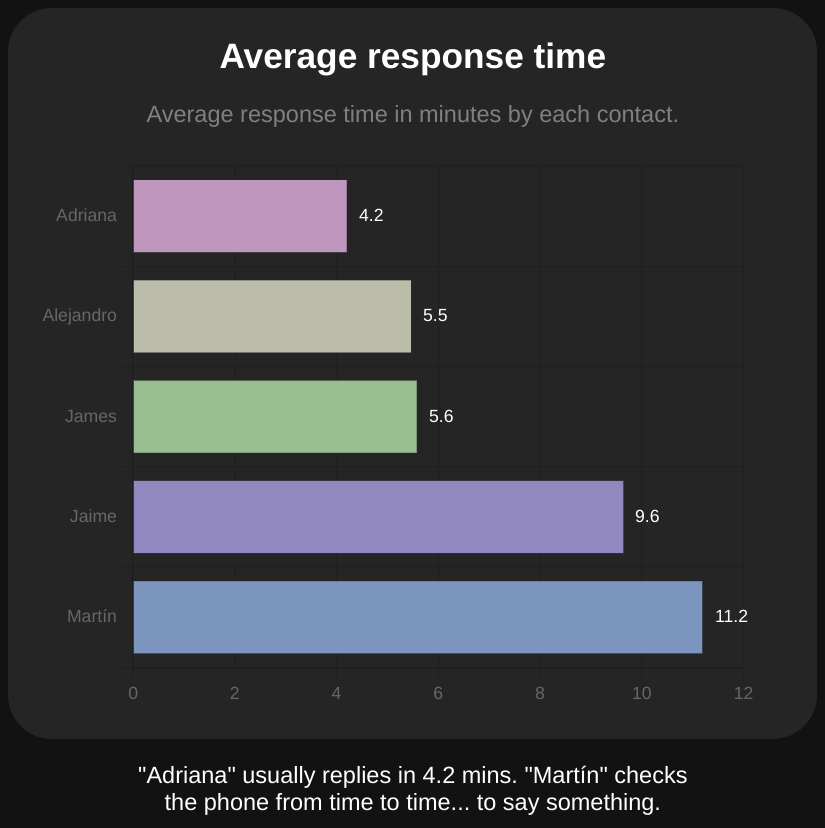
\includegraphics[width=6cm]{img/avg_response_time.png} }}
	\caption{Tiempo medio de respuesta}
	\label{fig:chap4:avg_response_time}
\end{figure}

Añadiendo esta figura a la anterior, podemos ver cómo Martín inicia pocas conversaciones y, además, suele tardar bastante en responder. Esto puede sugerir que está menos involucrado en el grupo.


\subsubsection{Contador de multimedia}

En caso de que existan objetos \acrshort{json} con el campo ``\textit{media\_type}'' distinto de \textit{undefined}, este submódulo cuenta cuántos archivos multimedia de cada tipo ha mandado cada contacto.


\begin{figure}[h]
	\centering
	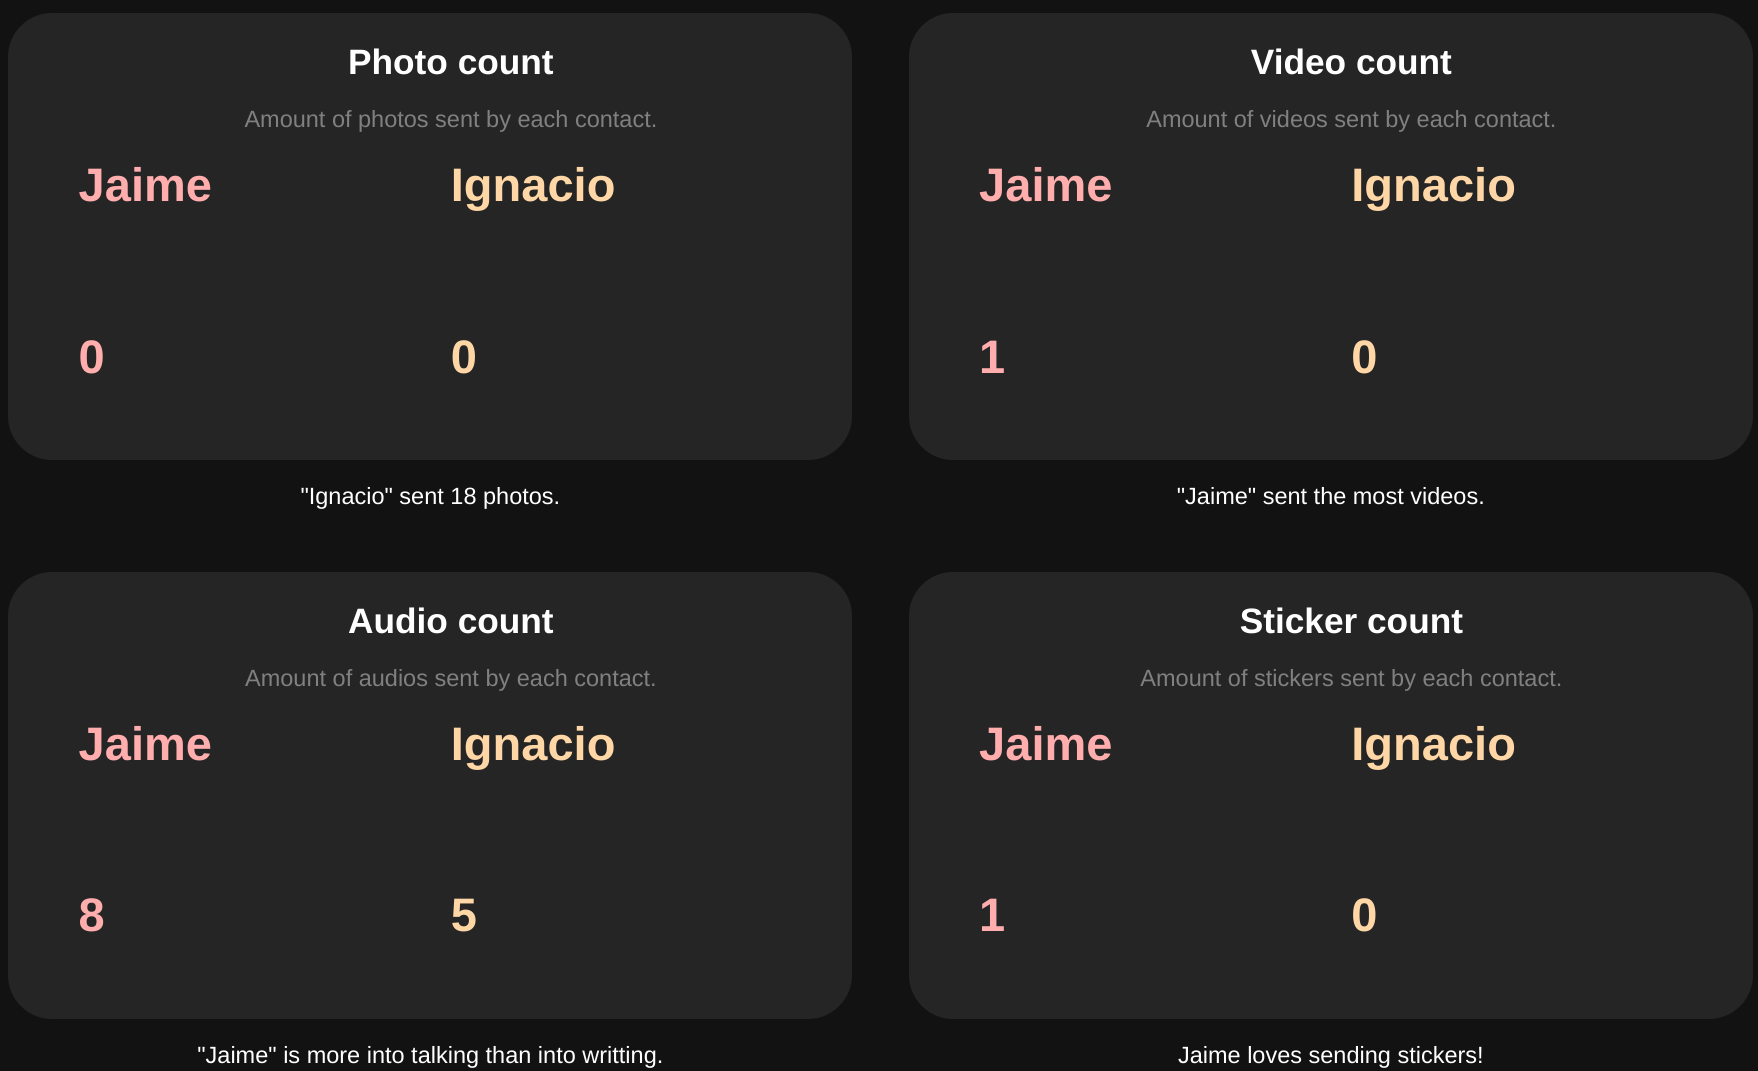
\includegraphics[width=0.8\textwidth]{img/media_count_individual.png}
	\caption{Contador de multimedia para chats individuales}
	\label{fig:chap4:media_count_individual}
\end{figure}


\begin{figure}[h]
	\centering
	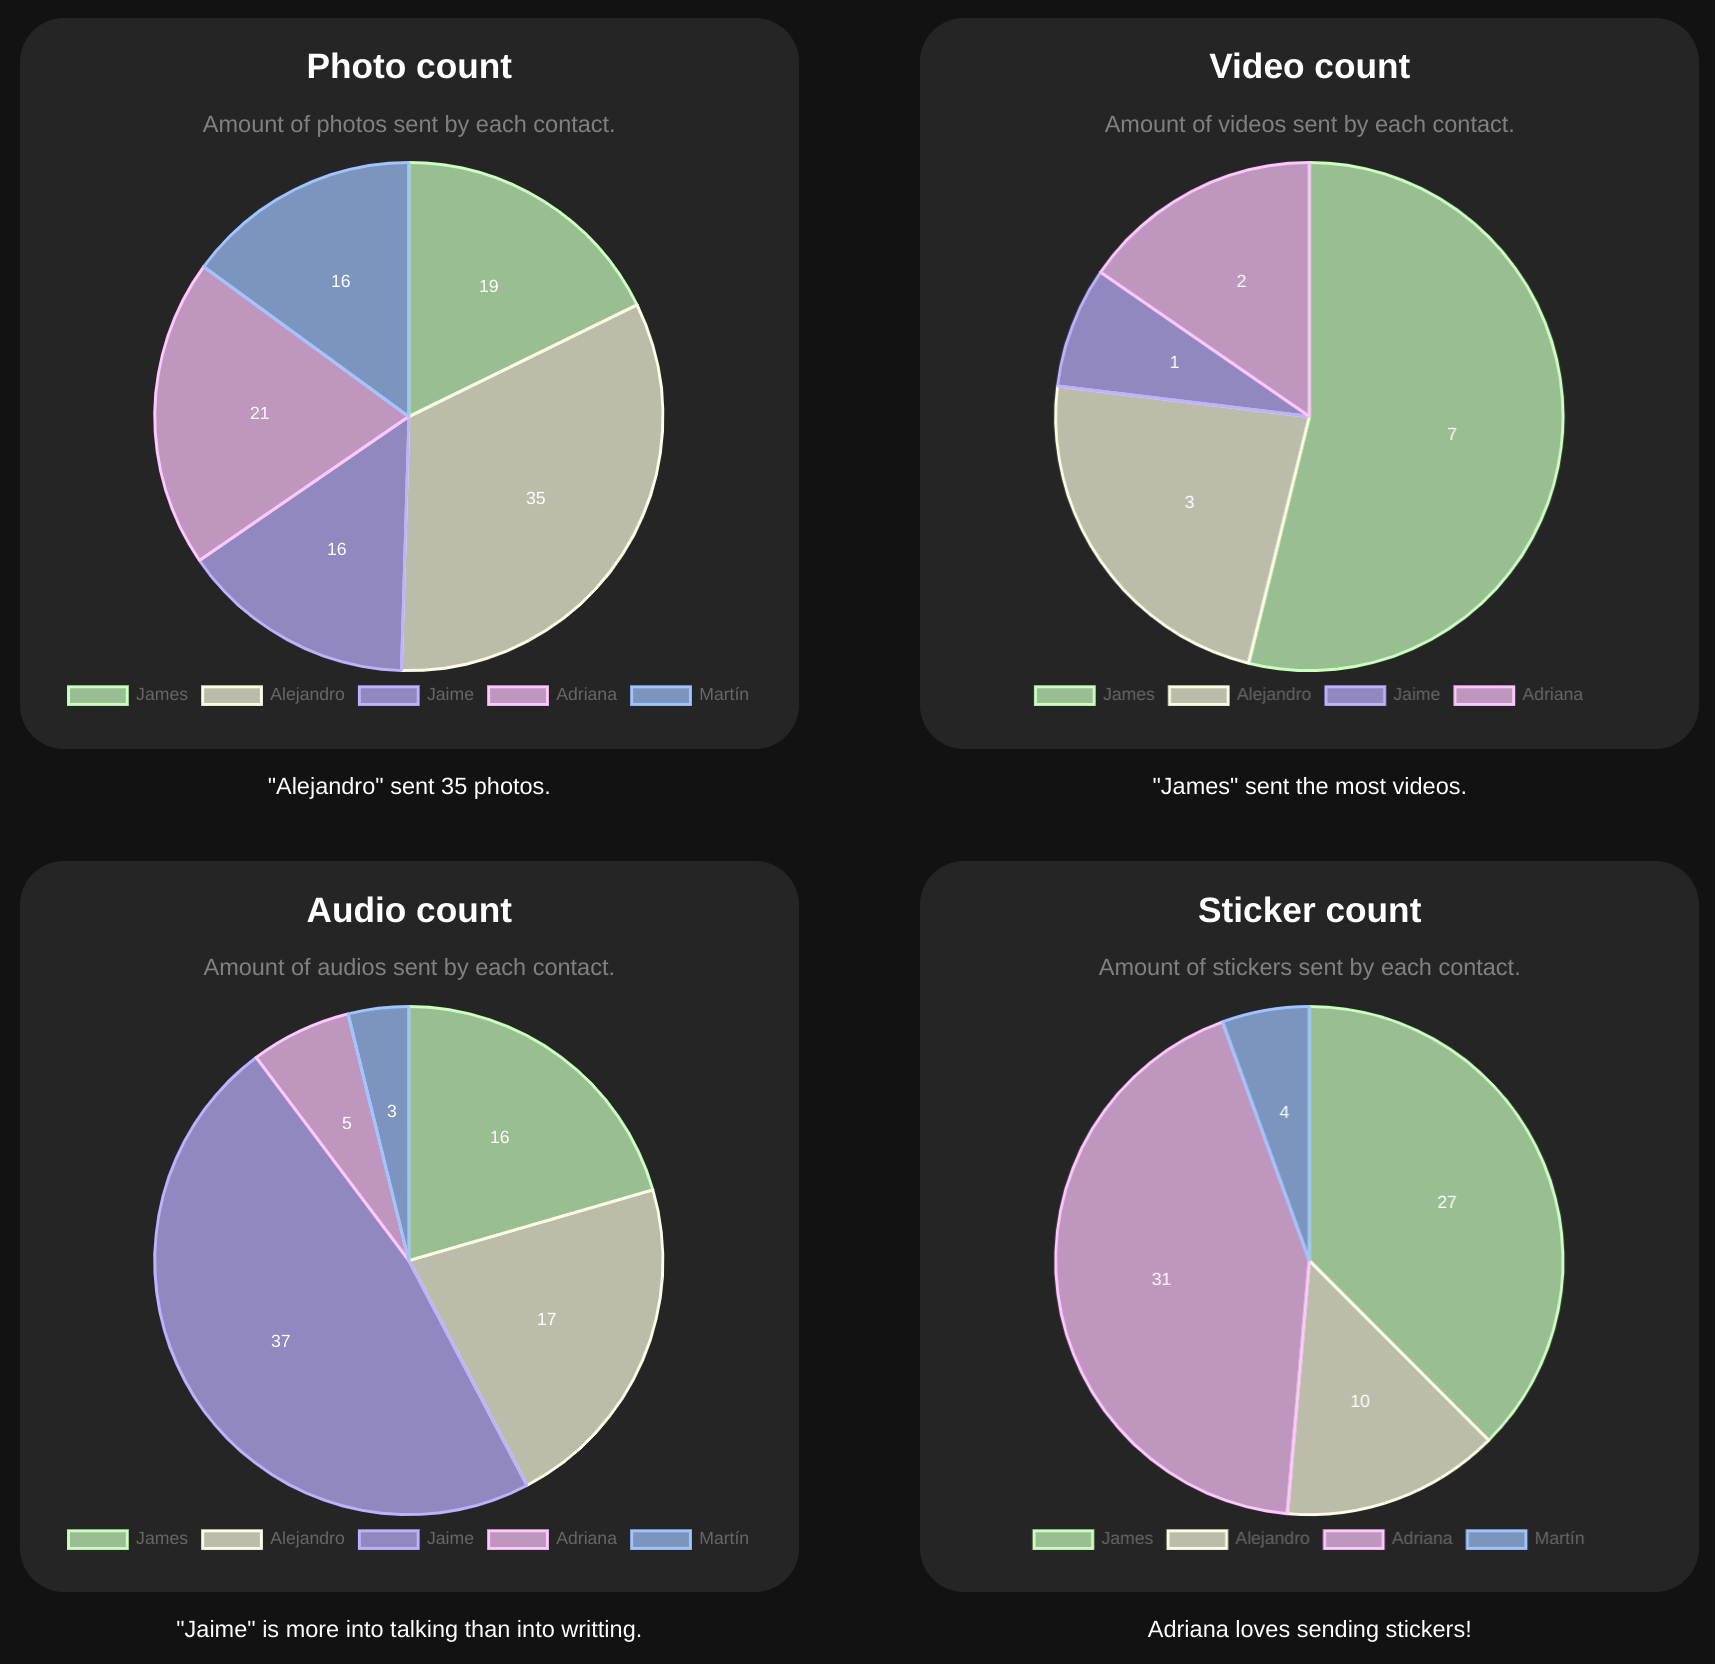
\includegraphics[width=0.8\textwidth]{img/media_count.png}
	\caption{Contador de multimedia para chats grupales}
	\label{fig:chap4:media_count}
\end{figure}

\subsubsection{Generador de estructuras de datos por día, hora y mes}

Para el gráfico de barras con el número de mensajes en el tiempo, \textit{ChartJS} necesita una estructura de datos para mensajes por día, siendo los días la variable independiente y el número de mensajes la variable dependiente.

\begin{figure}[H]
	\centering
	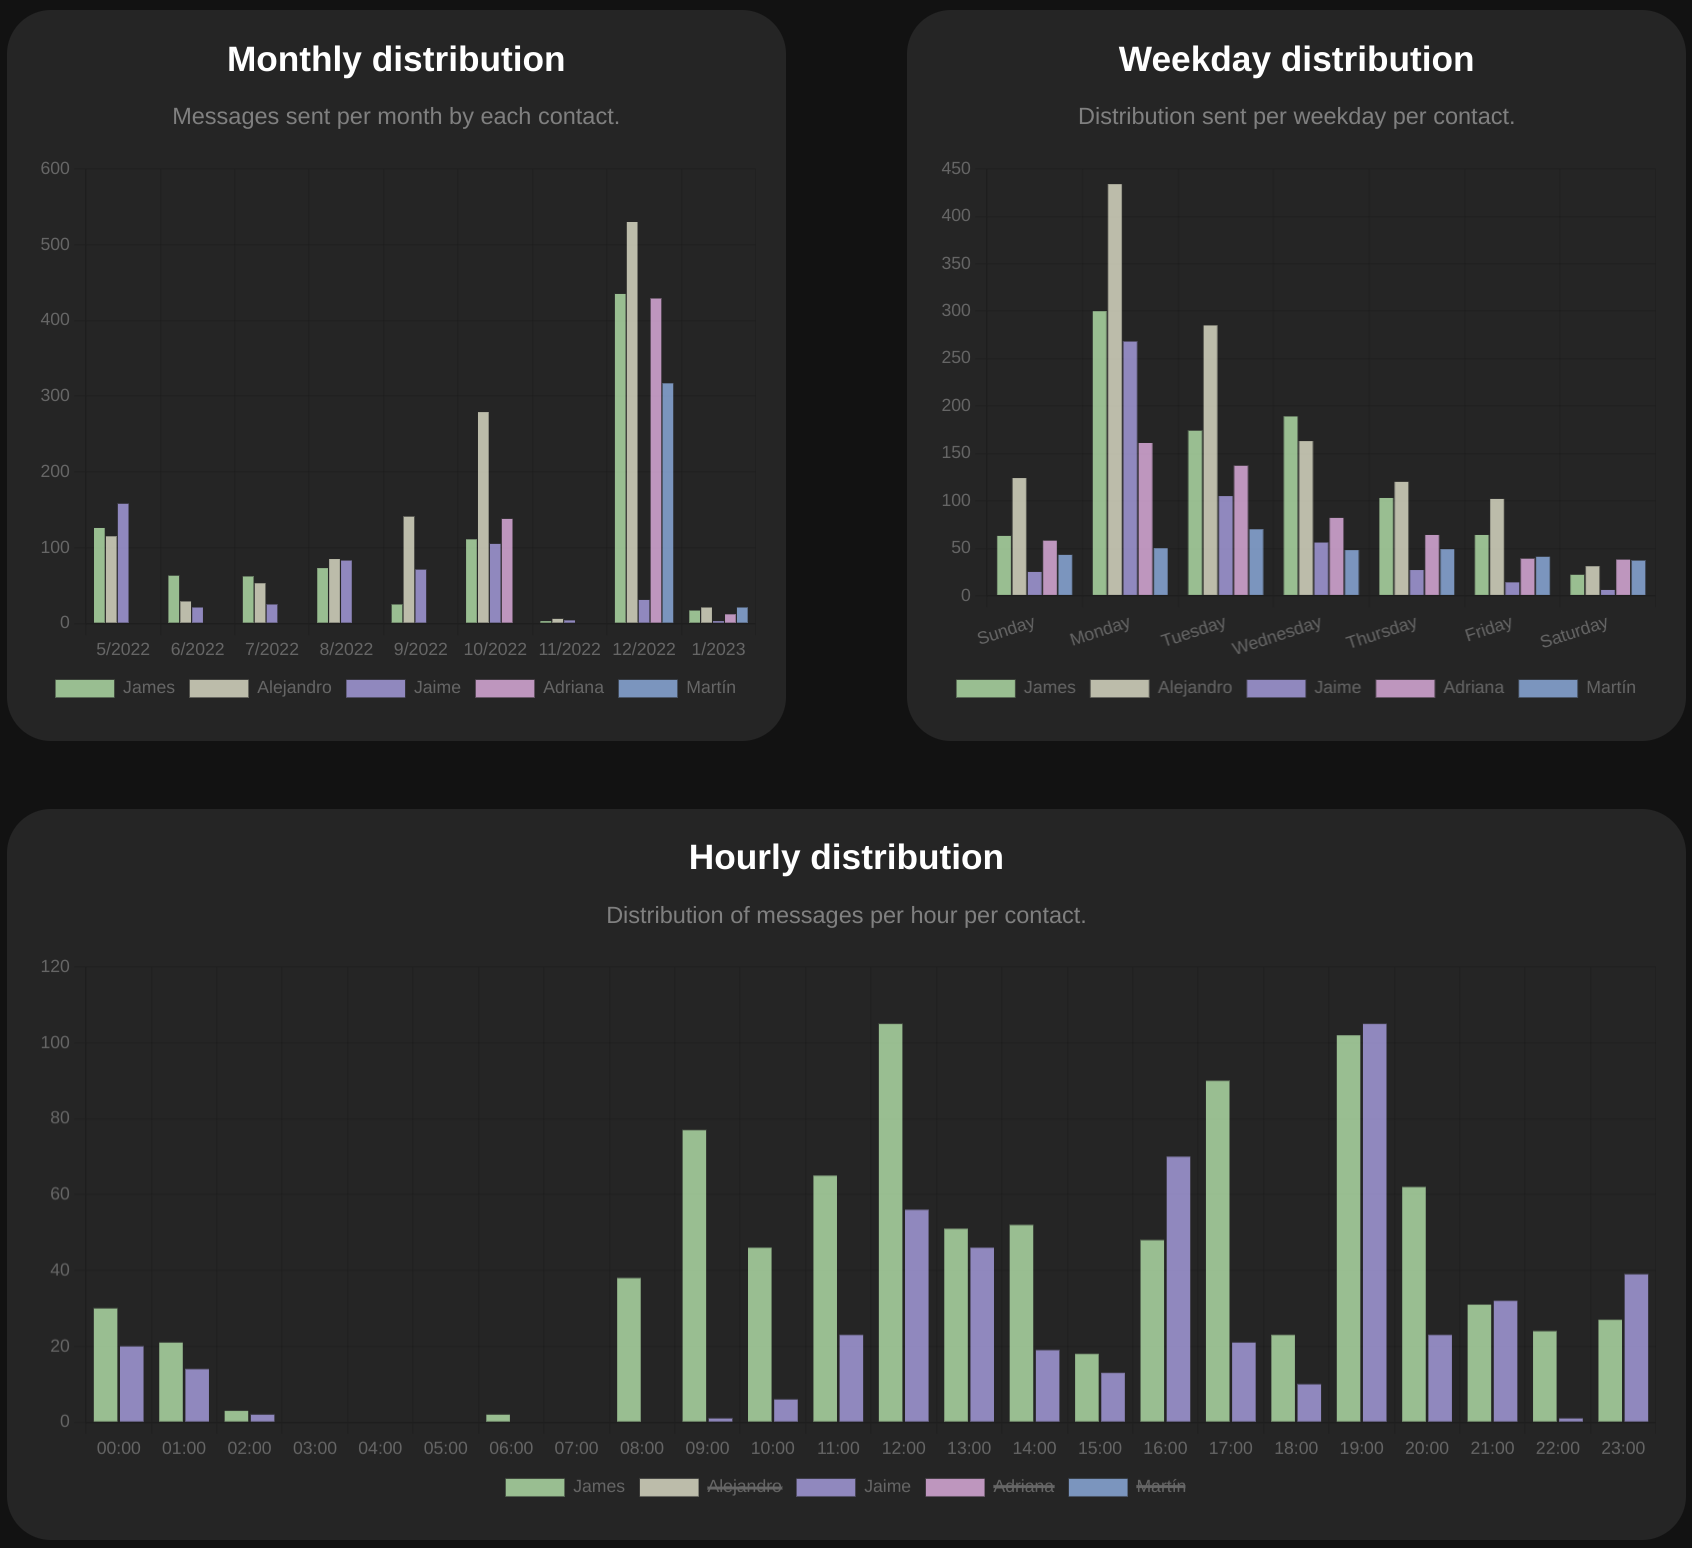
\includegraphics[width=0.8\textwidth]{img/time_distributions.png}
	\caption{Distribuciones en el tiempo}
	\label{fig:chap4:time_distributions}
\end{figure}

Se elige calcular y mostrar estas distribuciones puesto que ayudan a observar la evolución en el tiempo de la cantidad de mensajes intercambiados, así como los días de la semana más activos. Por ejemplo una pareja que pasa los fines de semana juntos tendrá menos mensajes los fines de semana. Por último, la distribución en las 24 horas del día ayuda a analizar las horas pico de conversación, así como las horas de final e inicio del día para cada contacto.

Para la distribución por horas en el día, se ha planteado también usar un gráfico de araña o radar, pero dicha opción se descartó al observar el solapamiento que tenía lugar con varios contactos.

En la figura podemos observar cómo el contacto Jaime comienza a mandar mensajes a las 9 de la mañana, mientras que James suele comenzar 2 horas antes: a las 7 de la mañana. Esto sugiere que James comienza antes el día, o Jaime no utiliza el móvil hasta las 9 de la mañana.

\subsubsection{Contador de palabras más repetidas}

Este submódulo procesa todas las palabras de los mensajes, elimina las palabras más comunes del español y el inglés, así como otros mensajes que WhatsApp añade, como \textit{Media ommited} o \textit{This message has been deleted}.

Las listas de palabras más comunes del español e inglés se han recopilado de distintas fuentes, combinado y eliminado repeticiones.

A la salida de este módulo, se muestra un diccionario con las palabras más repetidas y el número de veces que aparece cada una; información de la que hará uso la librería \textit{react-wordcloud}. Esta información resulta útil para resaltar los temas principales tratados en el chat.

Puede observarse en la \autoref{fig:chap4:word_emoji_cloud}

\subsubsection{Contador de emoticonos más usados}

Este módulo aplica una expresión regular unicode a todos los mensajes, seleccionando los emoticonos y contando el número de veces que aparecen. Posteriormente otra nube de palabras hace uso de esta información por medio de la librería \textit{react-wordcloud}.

\begin{figure}[H]
	\centering
	\subfloat[\centering Nube de palabras]{{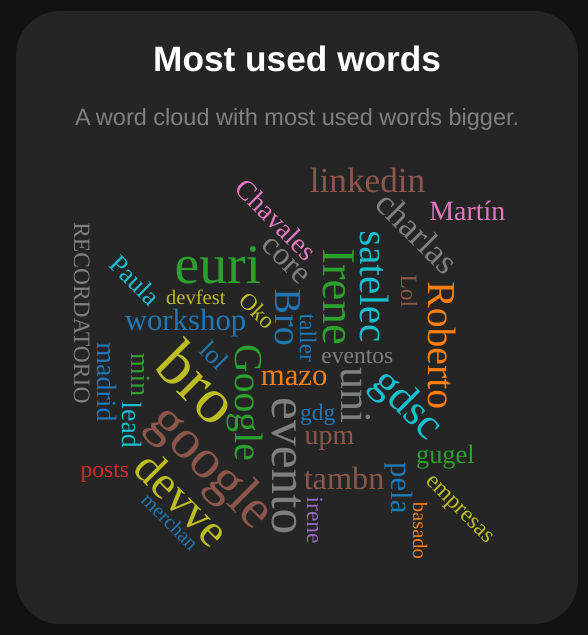
\includegraphics[width=6cm]{img/word_cloud.png} }}
	\qquad
	\subfloat[\centering Nube de emoticonos]{{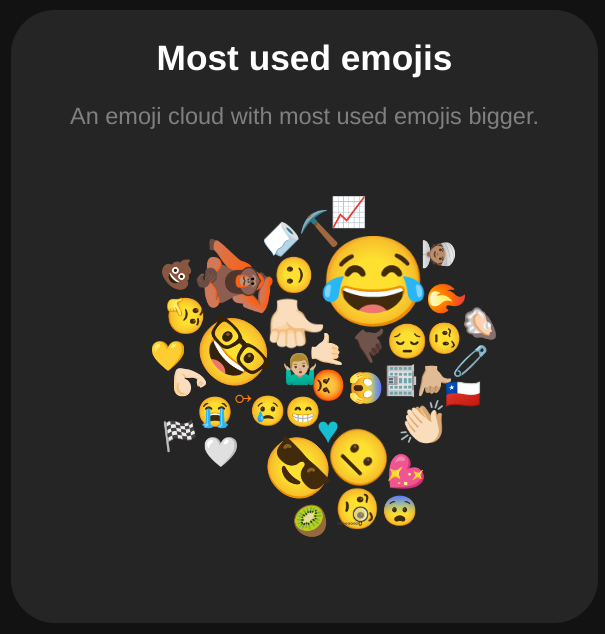
\includegraphics[width=6cm]{img/emoji_cloud.png} }}
	\caption{Nube de palabras y emoticonos}
	\label{fig:chap4:word_emoji_cloud}
\end{figure}

Se elige calcular y mostrar esta visualización puesto que los emoticonos constituyen en un chat la forma más similar a la expresión no verbal.

\section{Conclusión}

Con todo, si en un futuro se quiere extender la arquitectura propuesta a un modelo de cliente-servidor, siempre se puede añadir un tercer contenedor en la última capa de la \autoref{chap:architecture:server} que implemente lógica adicional. Sería también necesaria cierta modificación en el código del cliente para implementar peticiones a este nuevo servicio.


\chapter{Caso de estudio}
\label{chap:case-study}

\section{Introducción}
\label{sec:5:introduction}

En este capítulo vamos a describir los casos de uso principales de ChatStats. Estas descripciones cubrirán todas las funciones principales, así como una descripción detallada de los pasos a seguir y cómo usar la aplicación.

A lo largo de los casos de uso, iremos viendo la aplicación en distintos dispositivos y tamaños, pudiendo comprobar cómo la aplicación se adapta a la pantalla de una forma \textit{responsive}.

\section{Instalar aplicación en cliente}

En esta sección se explicará el proceso de instalación de ChatStats en un dispositivo con navegador con soporte para \acrfull{pwa}.

En primer lugar, el usuario accede a la web donde se aloja la aplicación. El navegador sugiere la instalación de la aplicación. El usuario pulsa sobre la sugerencia e instala la aplicación, que estará accesible desde el escritorio del dispositivo. La aplicación puede usarse sin acceso a Internet.


\begin{figure}[H]
	\centering
	\subfloat[\centering Acceso a ChatStats]{{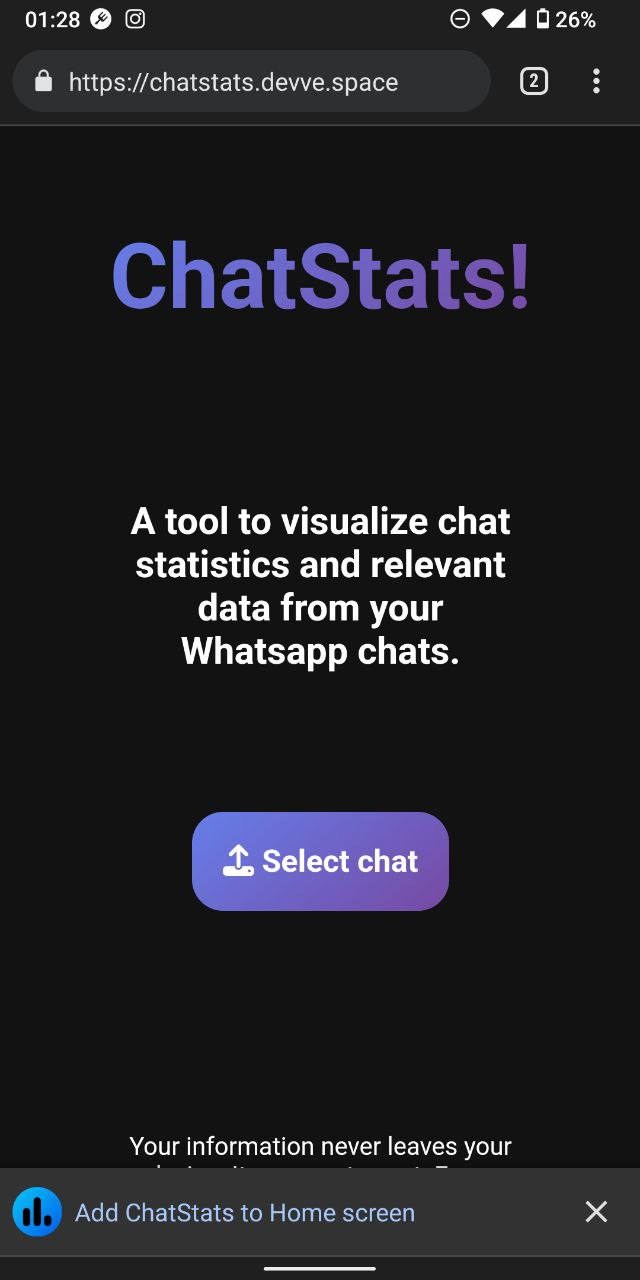
\includegraphics[width=3cm]{img/study_case/installation_1.jpg} }}
	\qquad
	\subfloat[\centering Instalación]{{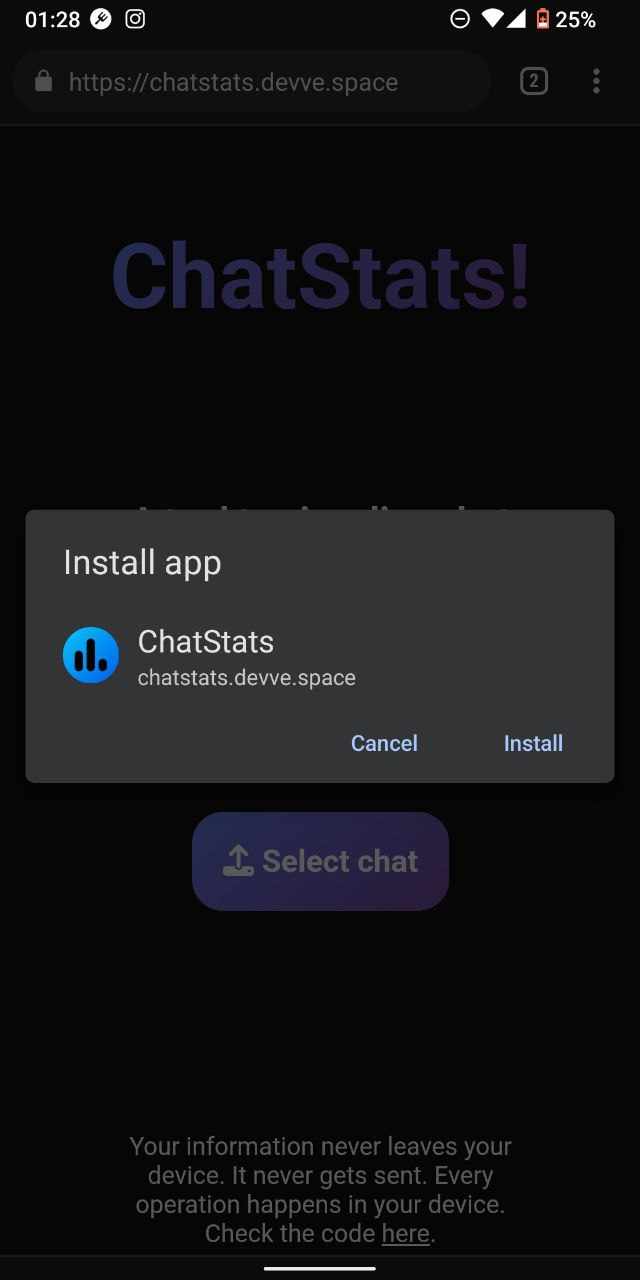
\includegraphics[width=3cm]{img/study_case/installation_2.jpg} }}
	\qquad
	\subfloat[\centering Colocación en escritorio]{{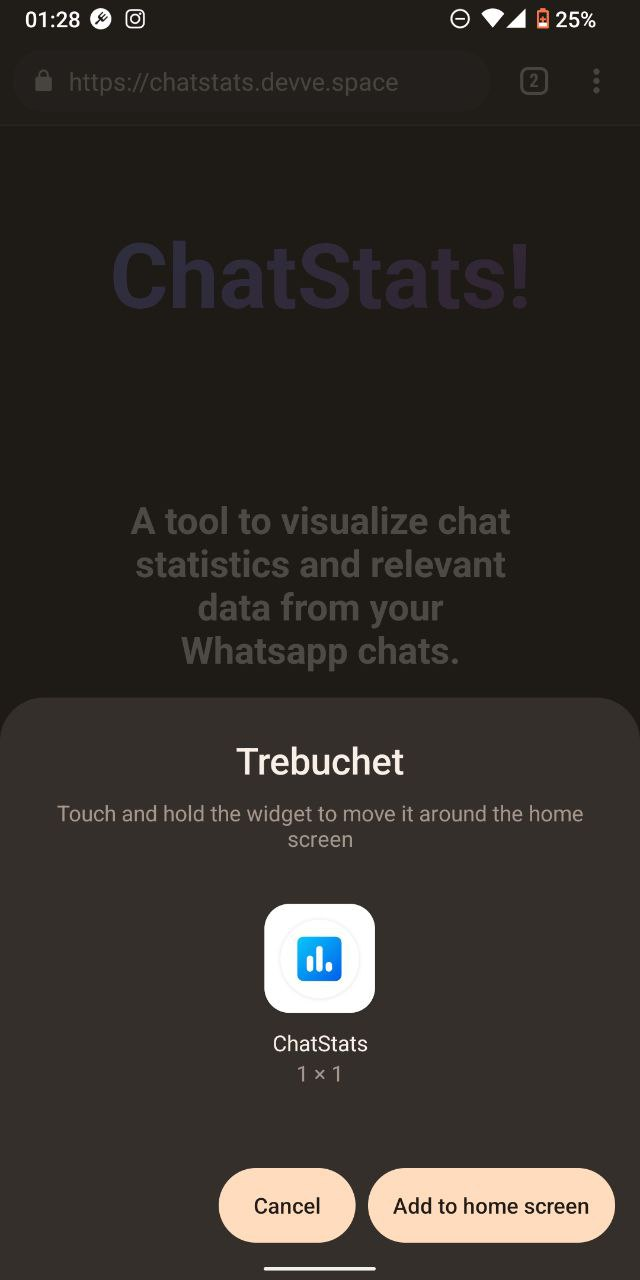
\includegraphics[width=3cm]{img/study_case/installation_3.jpg} }}
	\caption{Instalación de la aplicación \acrshort{pwa}}
	\label{fig:chap5:pwa_installation}
\end{figure}


\section{Importar datos en el sistema}

Durante este caso de uso, el usuario puede seleccionar un archivo para importar a ChatStats. El archivo puede ser de texto plano, \textit{zip} o \acrshort{json}. En caso de ser otro tipo de archivo, ChatStats alerta al usuario y elimina la selección.

\begin{figure}[H]
	\centering
	\subfloat[\centering Selección de fichero]{{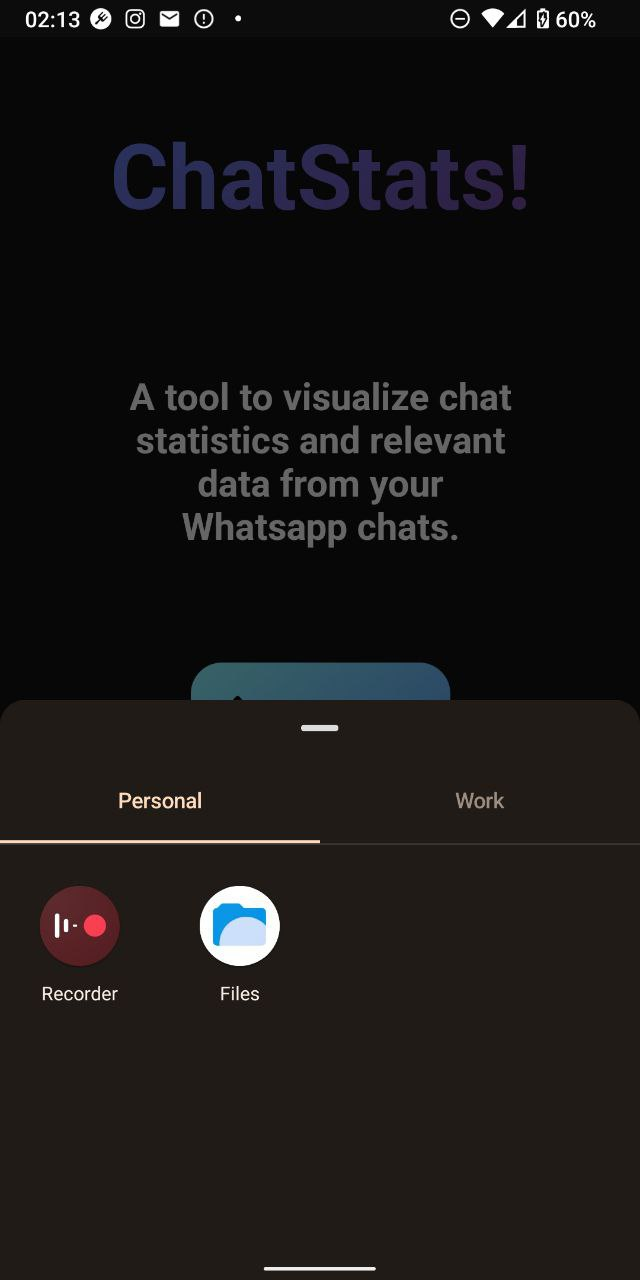
\includegraphics[width=3cm]{img/study_case/import_1.jpg} }}
	\qquad
	\subfloat[\centering Fichero válido seleccionado]{{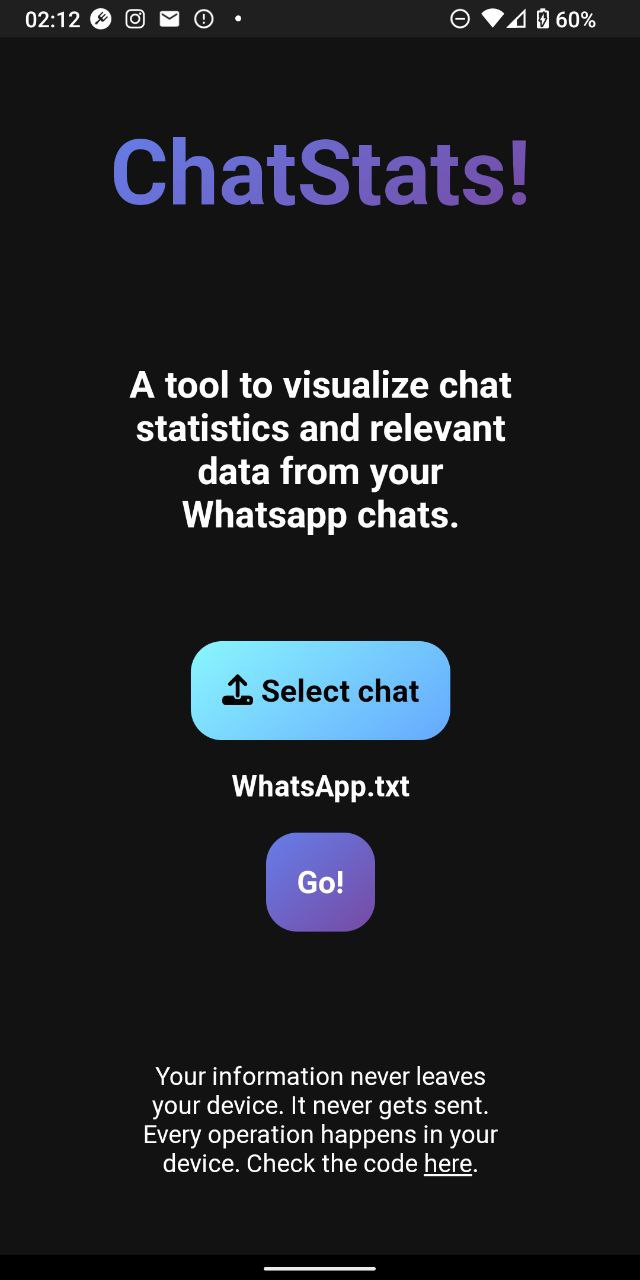
\includegraphics[width=3cm]{img/study_case/import_2.jpg} }}
	\qquad
	\subfloat[\centering Fichero no válido seleccionado]{{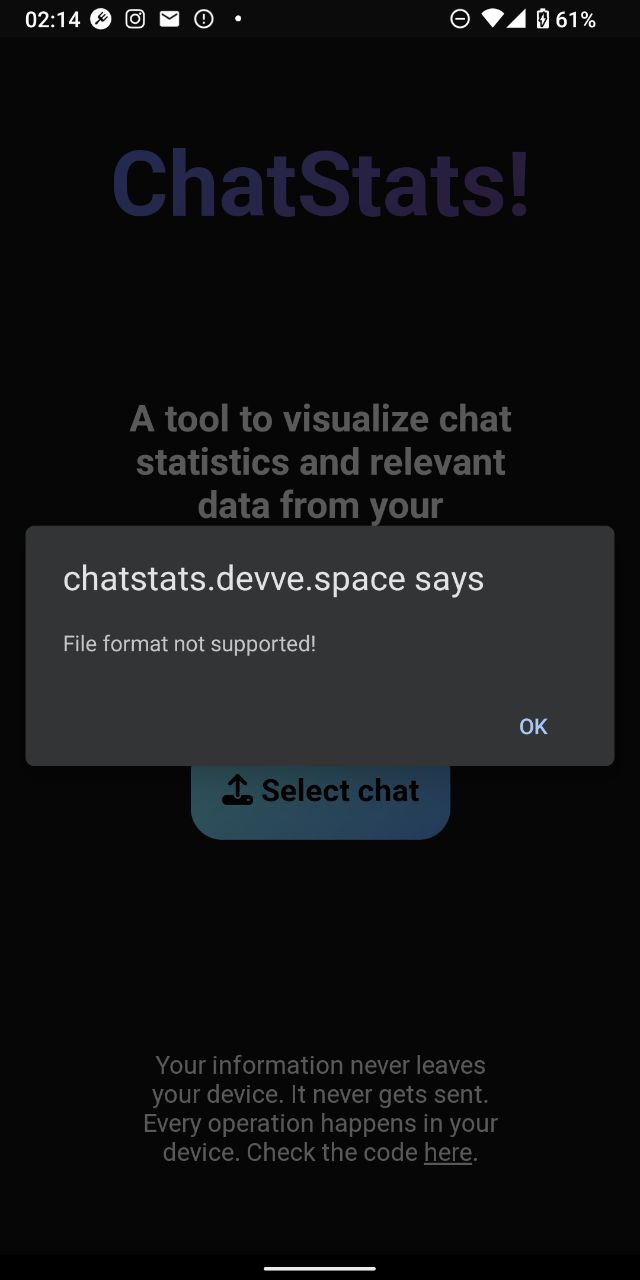
\includegraphics[width=3cm]{img/study_case/import_3.jpg} }}
	\caption{Importar datos en el sistema}
	\label{fig:chap5:import}
\end{figure}


\section{Visualización de chat grupal e individual}

\subsection{Cálculo de las estadísticas}

Durante esta pantalla, el cliente está ejecutando todos los flujos descritos en el \autoref{chap:architecture}. Se muestra una animación de carga para hacer saber al usuario que el cliente está realizando operaciones.

\begin{figure}[H]
	\centering
	\subfloat[\centering Inicio del cálculo]{{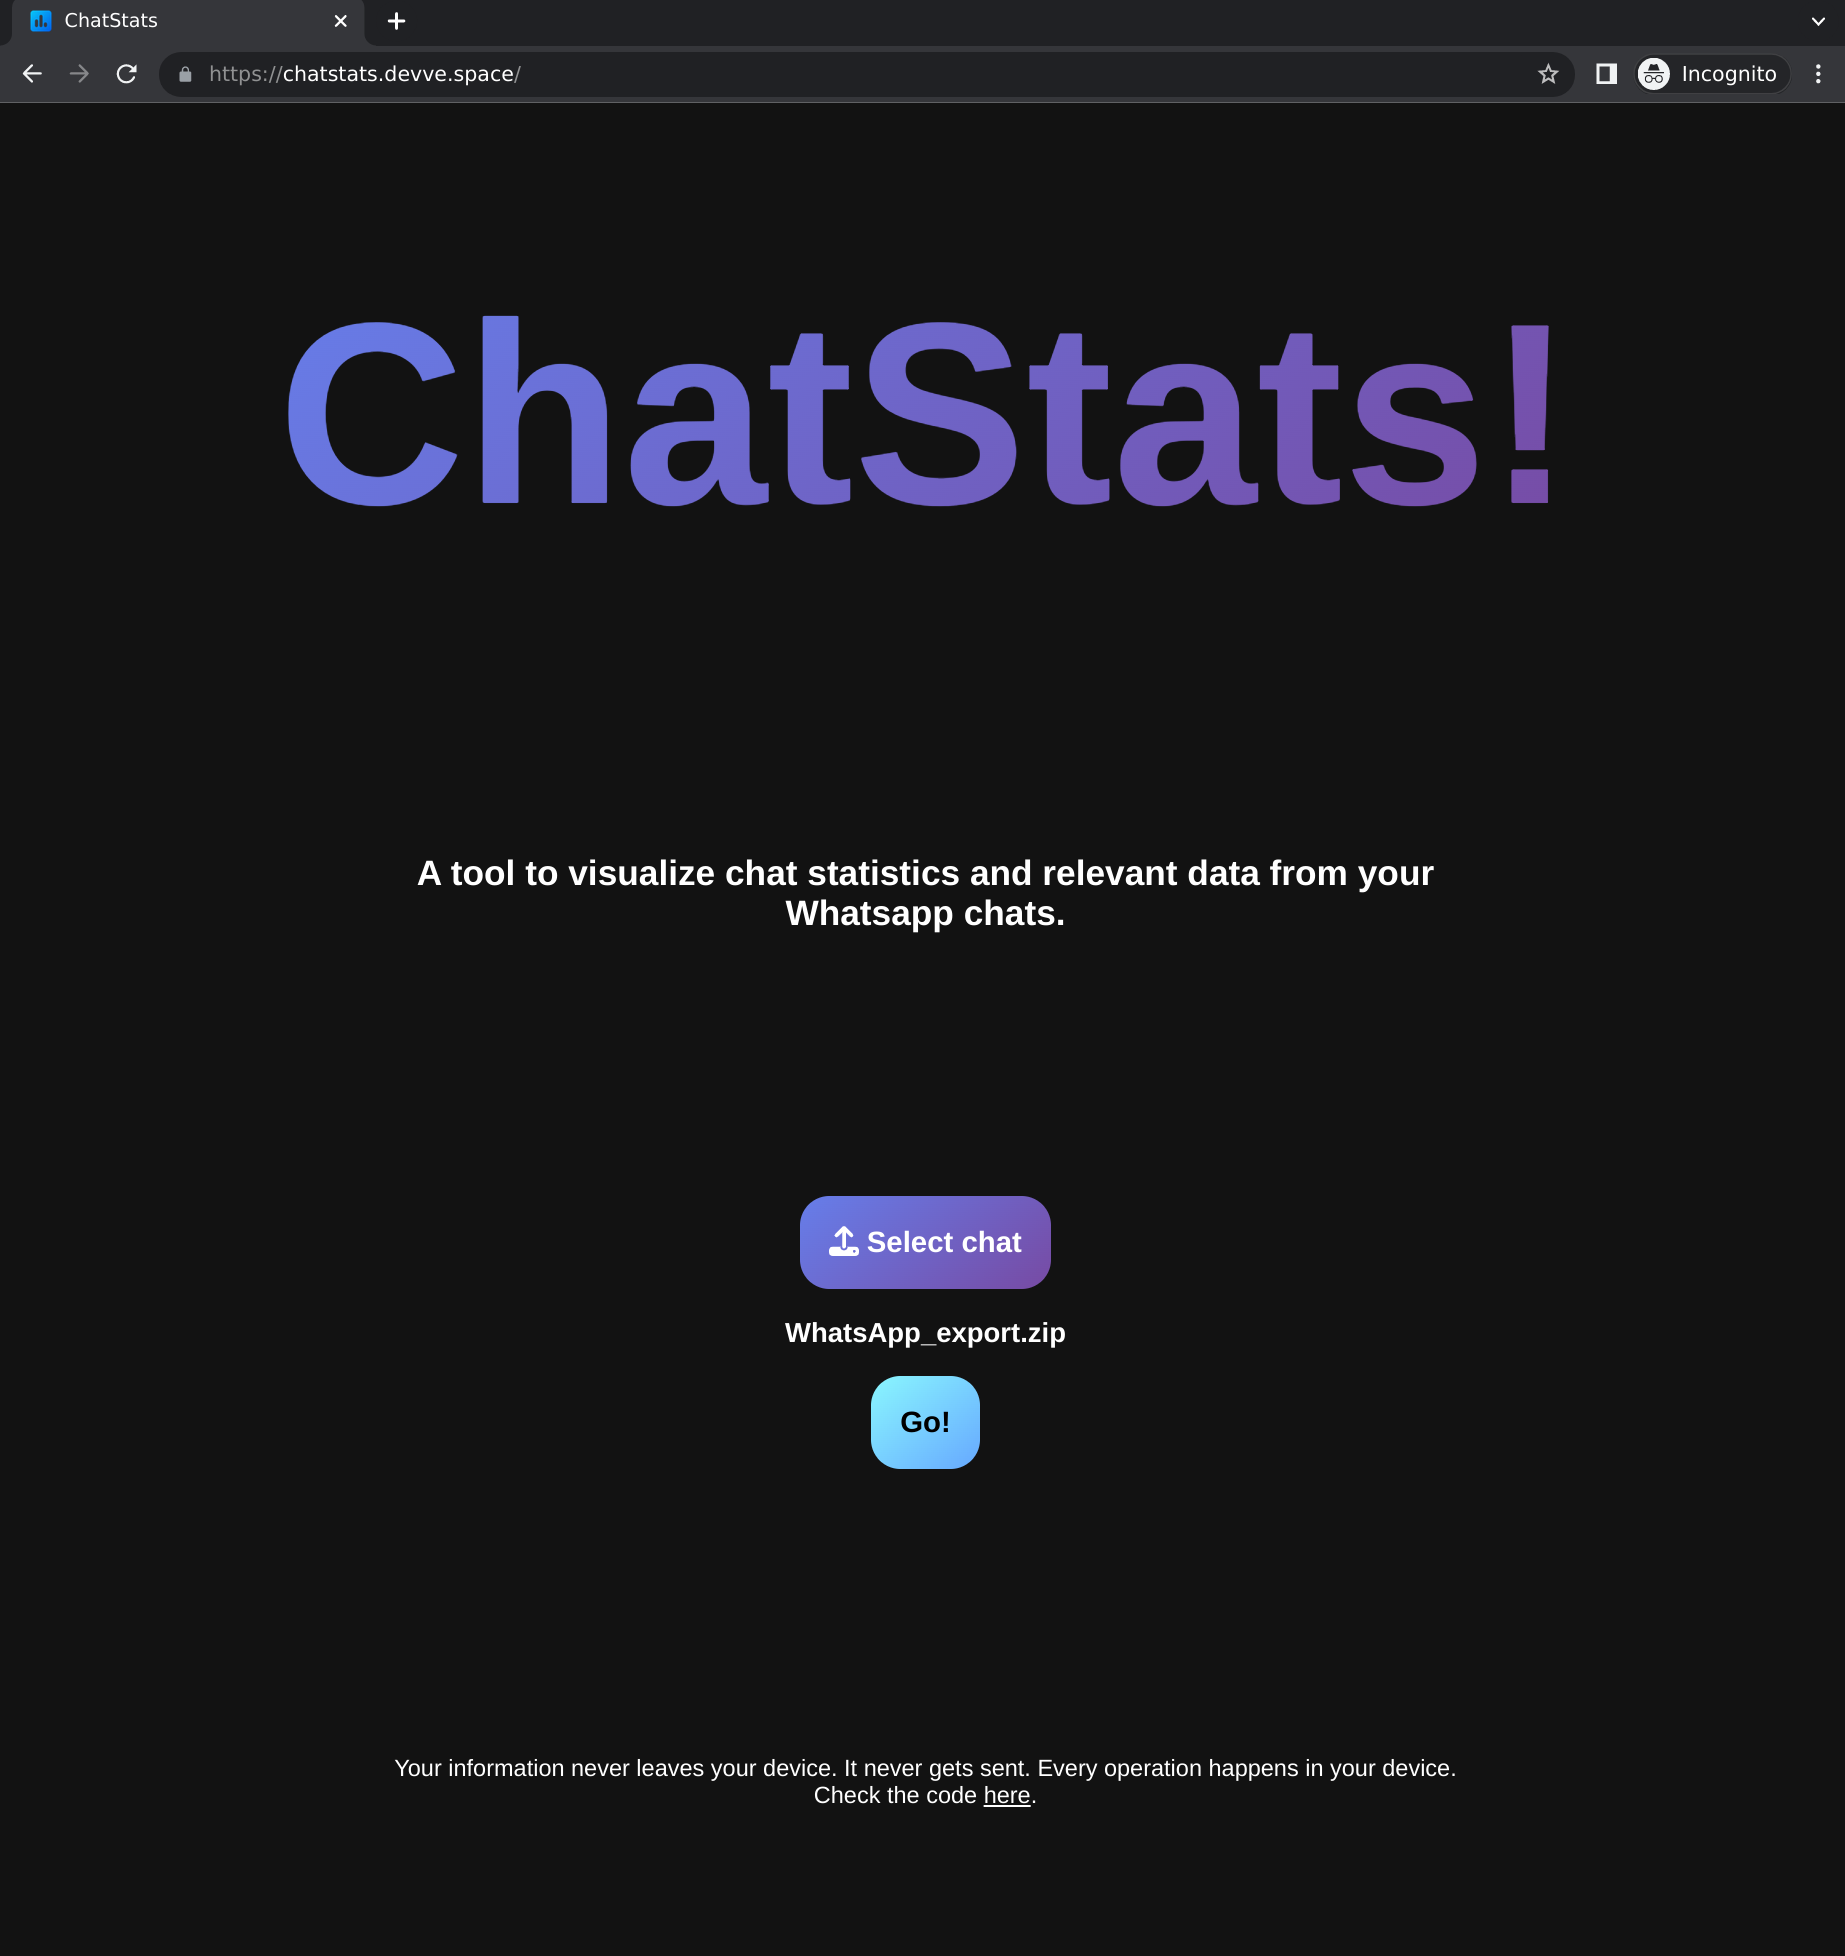
\includegraphics[width=7.1cm]{img/study_case/metrics_calc_1.png} }}
	\qquad
	\subfloat[\centering Carga durante el cálculo de métricas]{{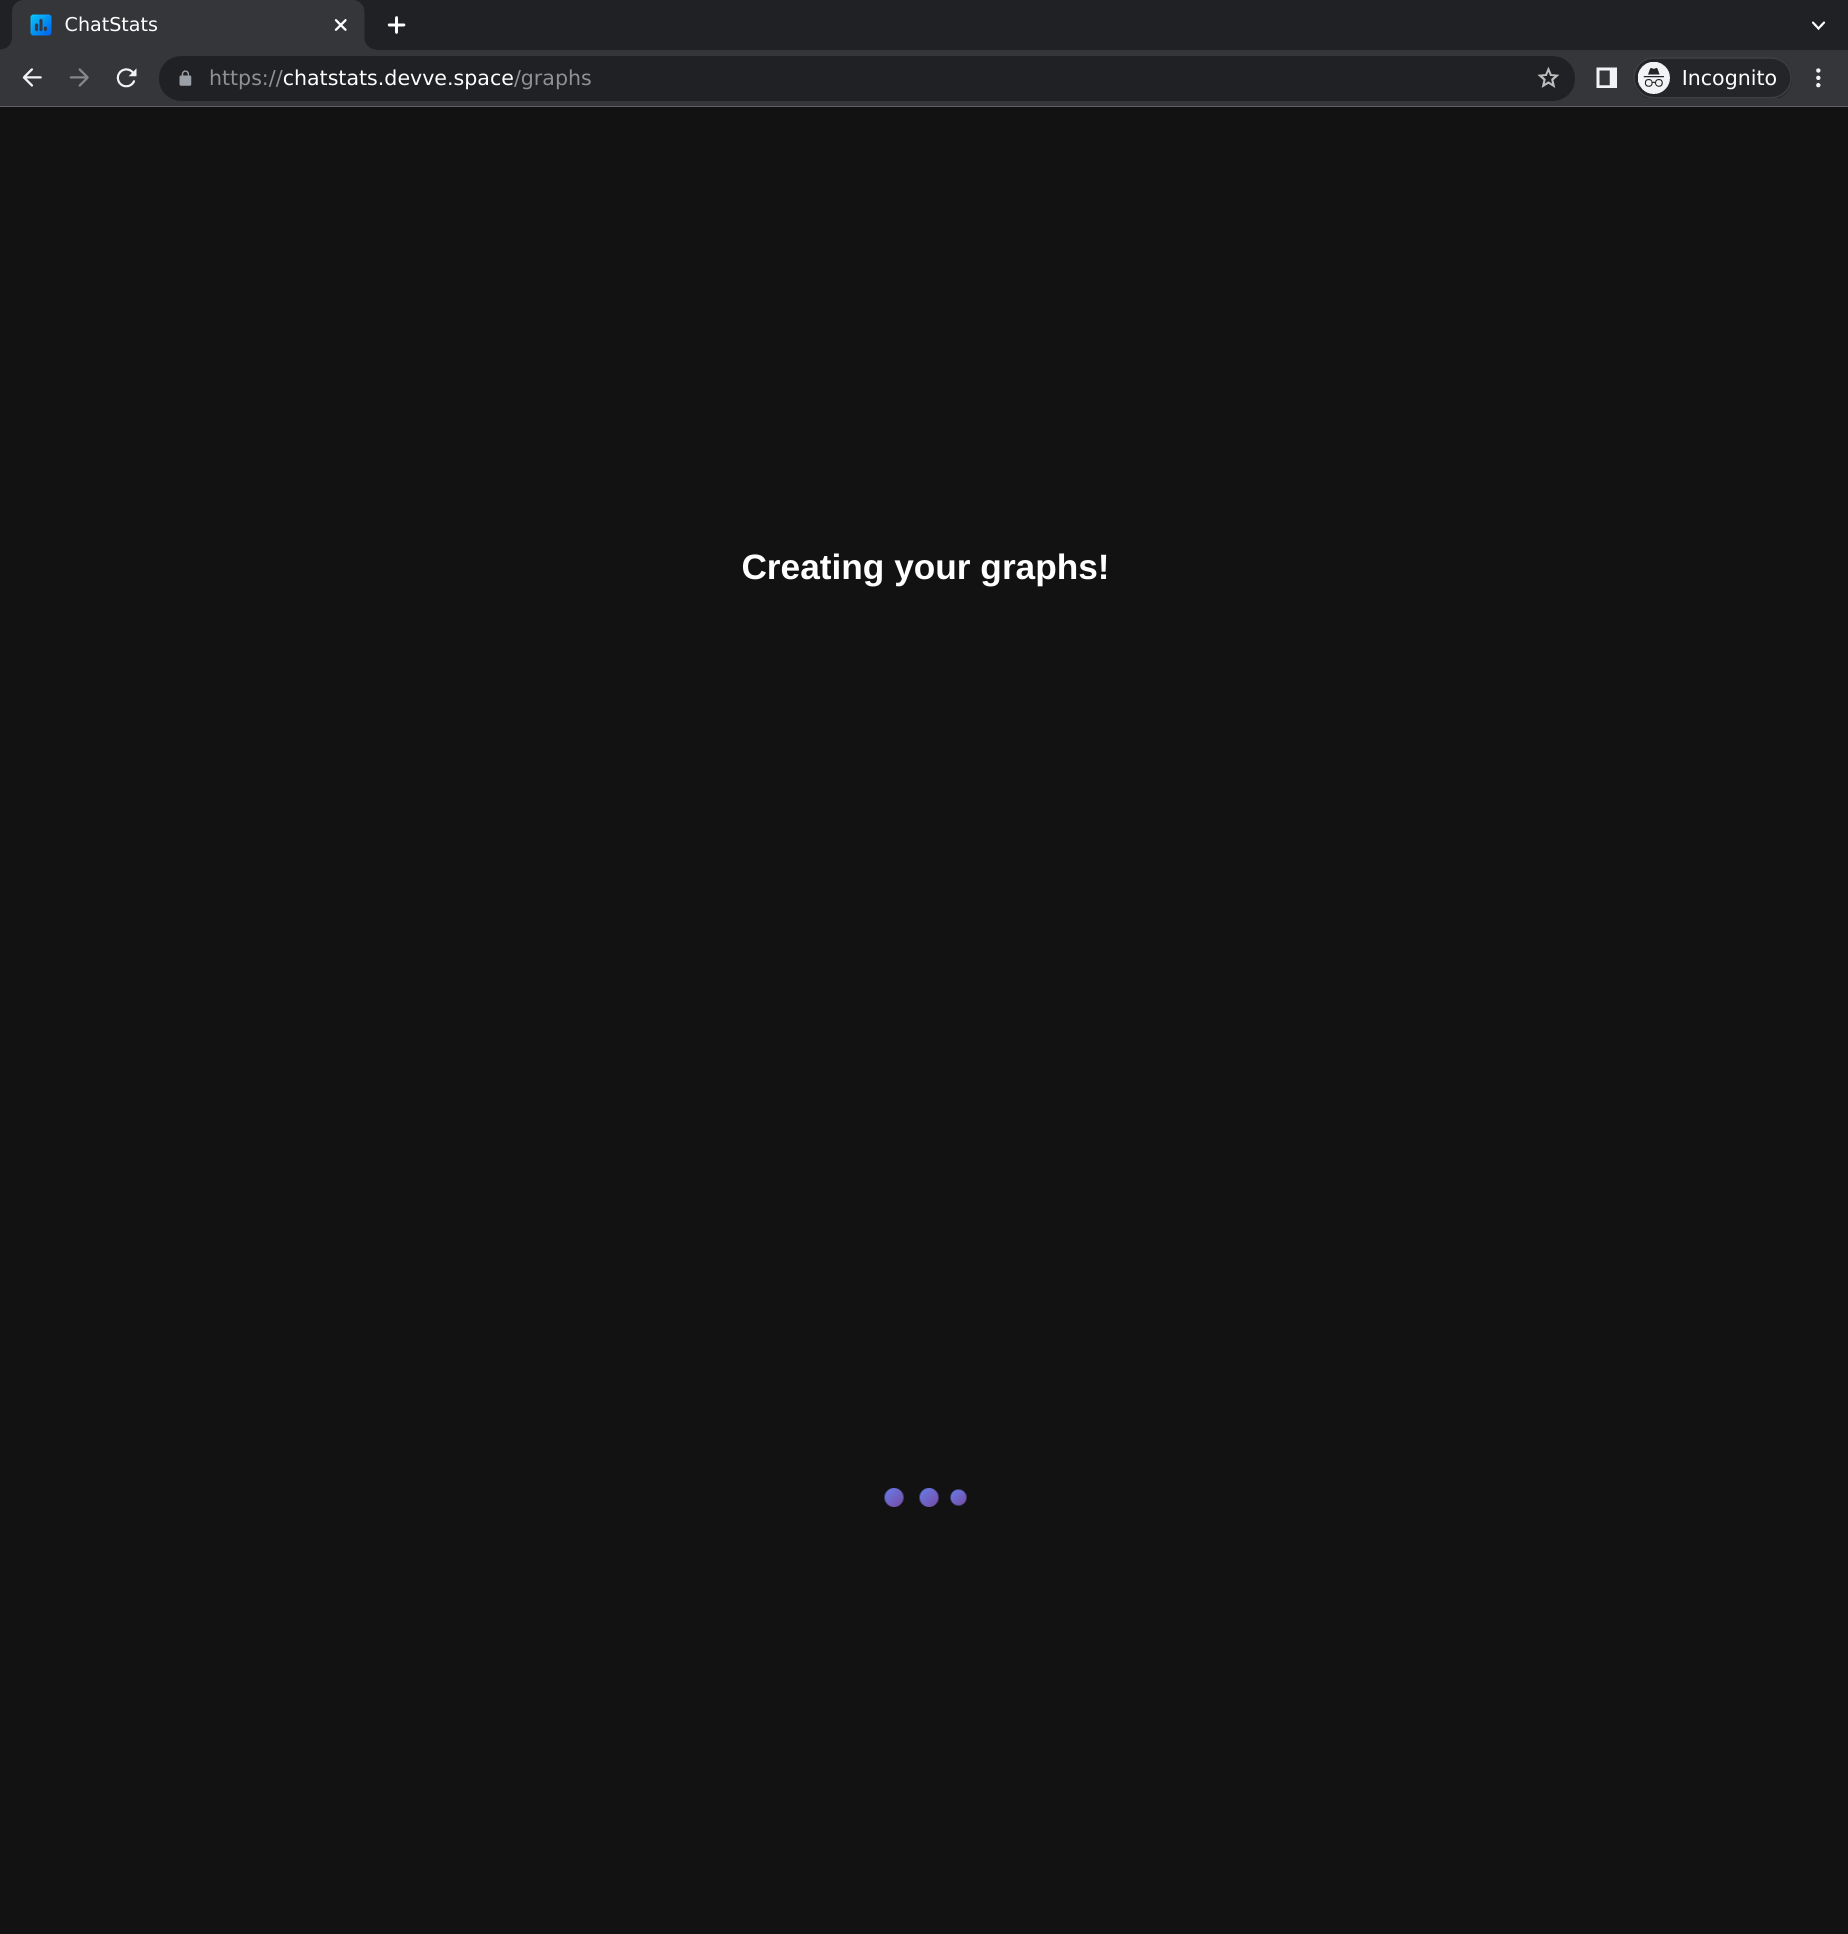
\includegraphics[width=7.1cm]{img/study_case/metrics_calc_2.png} }}
	\caption{Cálculo de métricas}
	\label{fig:chap5:calc}
\end{figure}


\subsection{Visualización de chat grupal e individual}

En esta página se muestran numerosos gráficos descritos durante la arquitectura, por los que el usuario puede desplazarse mediante la navegación vertical.

En el primer grupo de gráficos de la \autoref{fig:chap5:viz_grupal} (a) observamos el recuento de mensajes, palabras y caracteres para cada contacto. En este caso, podemos apreciar como los usuarios ``Alejandro'' y ``James'', en azul y morado respectivamente, constituyen casi un tercio de la conversación.

En el grupo de gráficos (b), en la \autoref{fig:chap5:viz_grupal} podemos observar la media de palabras por mensaje, así como la media de caracteres. De ellos podemos concluir, en este ejemplo, que todos los contactos escriben en media mensajes del mismo tamaño. En este grupo se incluye también un gráfico que indica el número de veces que cada contacto ha iniciado la conversación; así como el tiempo medio de respuesta de cada uno. Estos datos pueden ser muy útiles para medir el interés de los contactos por el chat en cuestión, así como qué contacto tiene mayor iniciativa al diálogo. Para nuestro caso de ejemplo, se observa que ``Alejandro'' suele comenzar la conversación, así como que Adriana es muy rápida respondiendo.

Continuando con el grupo de gráficos (c), podemos observar el número de archivos multimedia de cada tipo que ha enviado cada contacto. Aquí vemos que ``Adriana'' manda muchas pegatinas o \textit{stickers}, mientras que ``Jaime'' acostumbra a mandar más audios.

En el grupo de gráficos (d), podemos observar las distribución de los mensajes en los meses, en los días de la semana y en las horas del día. Anotamos que diciembre de 2022 fue el mes más activo del grupo y que los lunes suelen tener mayor actividad (que va decayendo a lo largo de la semana). Cabe comentar que en todos los gráficos anteriores se pueden descartar contactos en la representación. Es por eso que, quedándonos con ``James'' y ``Jaime'', podemos observar que ``James'' suele comenzar a enviar mensajes una hora antes que ``Jaime''.

Finalmente, en el grupo de gráficos (e) podemos observar las palabras clave más frecuentes del chat, así como los emoticonos. Estos nos permiten conocer rápidamente los temas principales de conversación, que son, en este caso: \textit{Google}, \textit{GDSC (Google Developers Student Club)} y \textit{evento}, entre otros. Asimismo, los emoticonos nos permiten conocer las principales reacciones no verbales que tienen lugar en la conversación.

\vspace{8mm}

Para el caso de chats individuales, se elimina la necesidad de la utilización de un gráfico circular y se muestran los números calculados directamente. Los gráficos de barras para las distribuciones en el tiempo no varían. Se muestran algunas diferencias en la \autoref{fig:chap5:viz_individual}.

\begin{figure}[h]
	\centering
	\subfloat[\centering Número de mensajes, número de palabras y número de caracteres]{{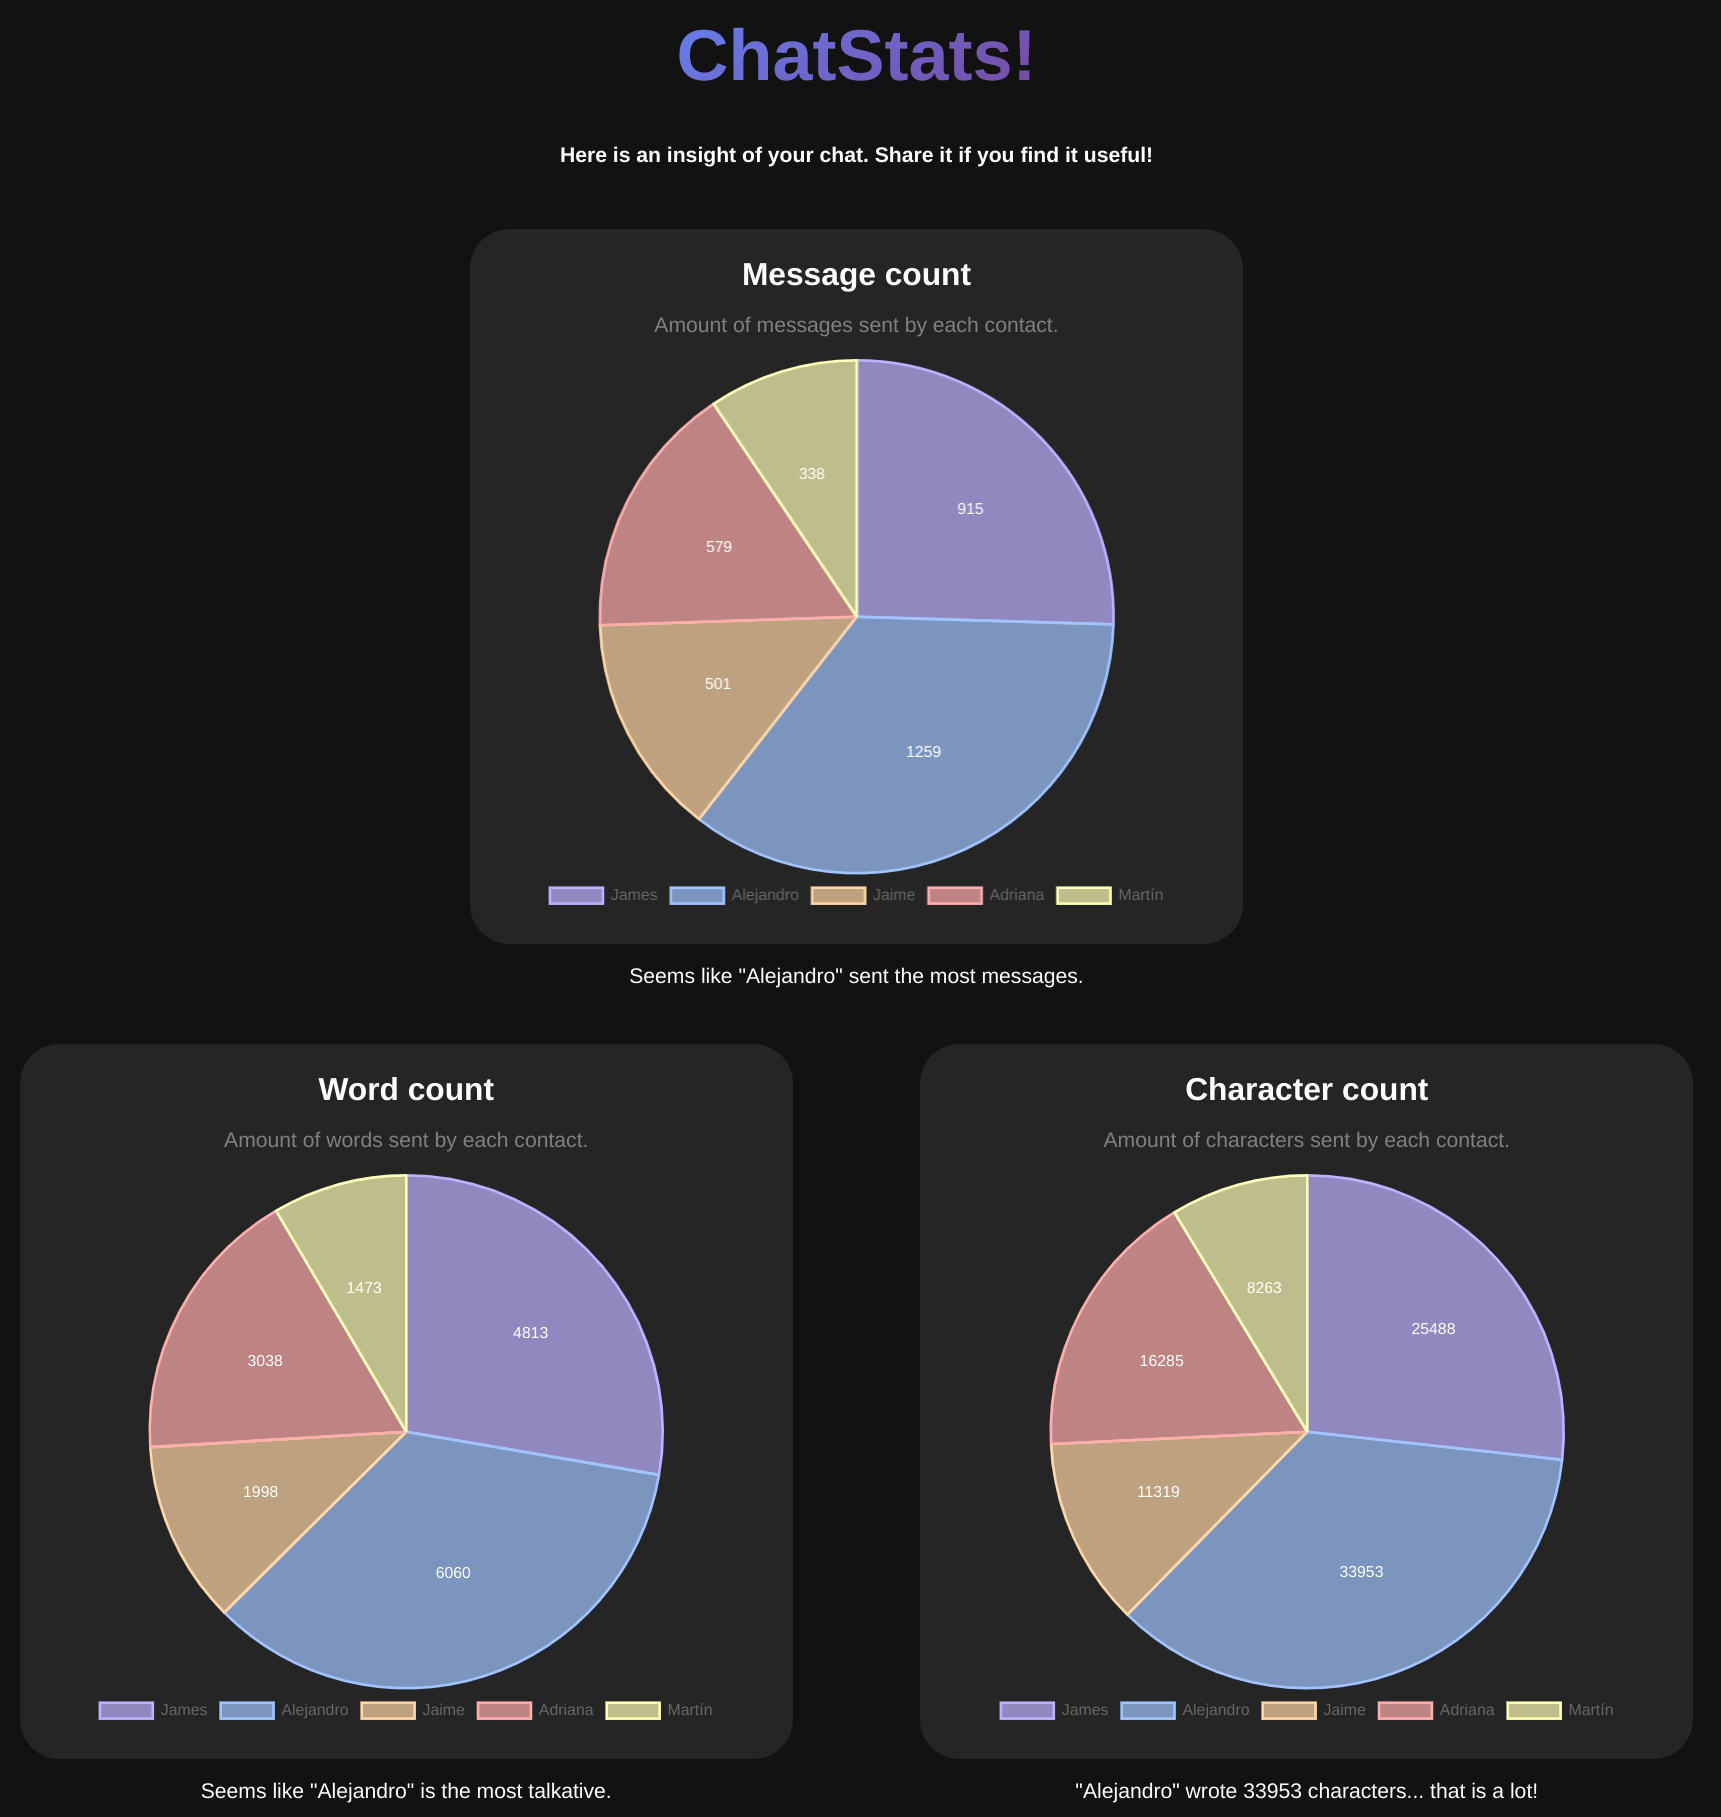
\includegraphics[width=7cm]{img/study_case/screen_1.png} }}
	\qquad
	\subfloat[\centering Media de palabras, media de caracteres, conversaciones iniciadas y tiempo medio de respuesta]{{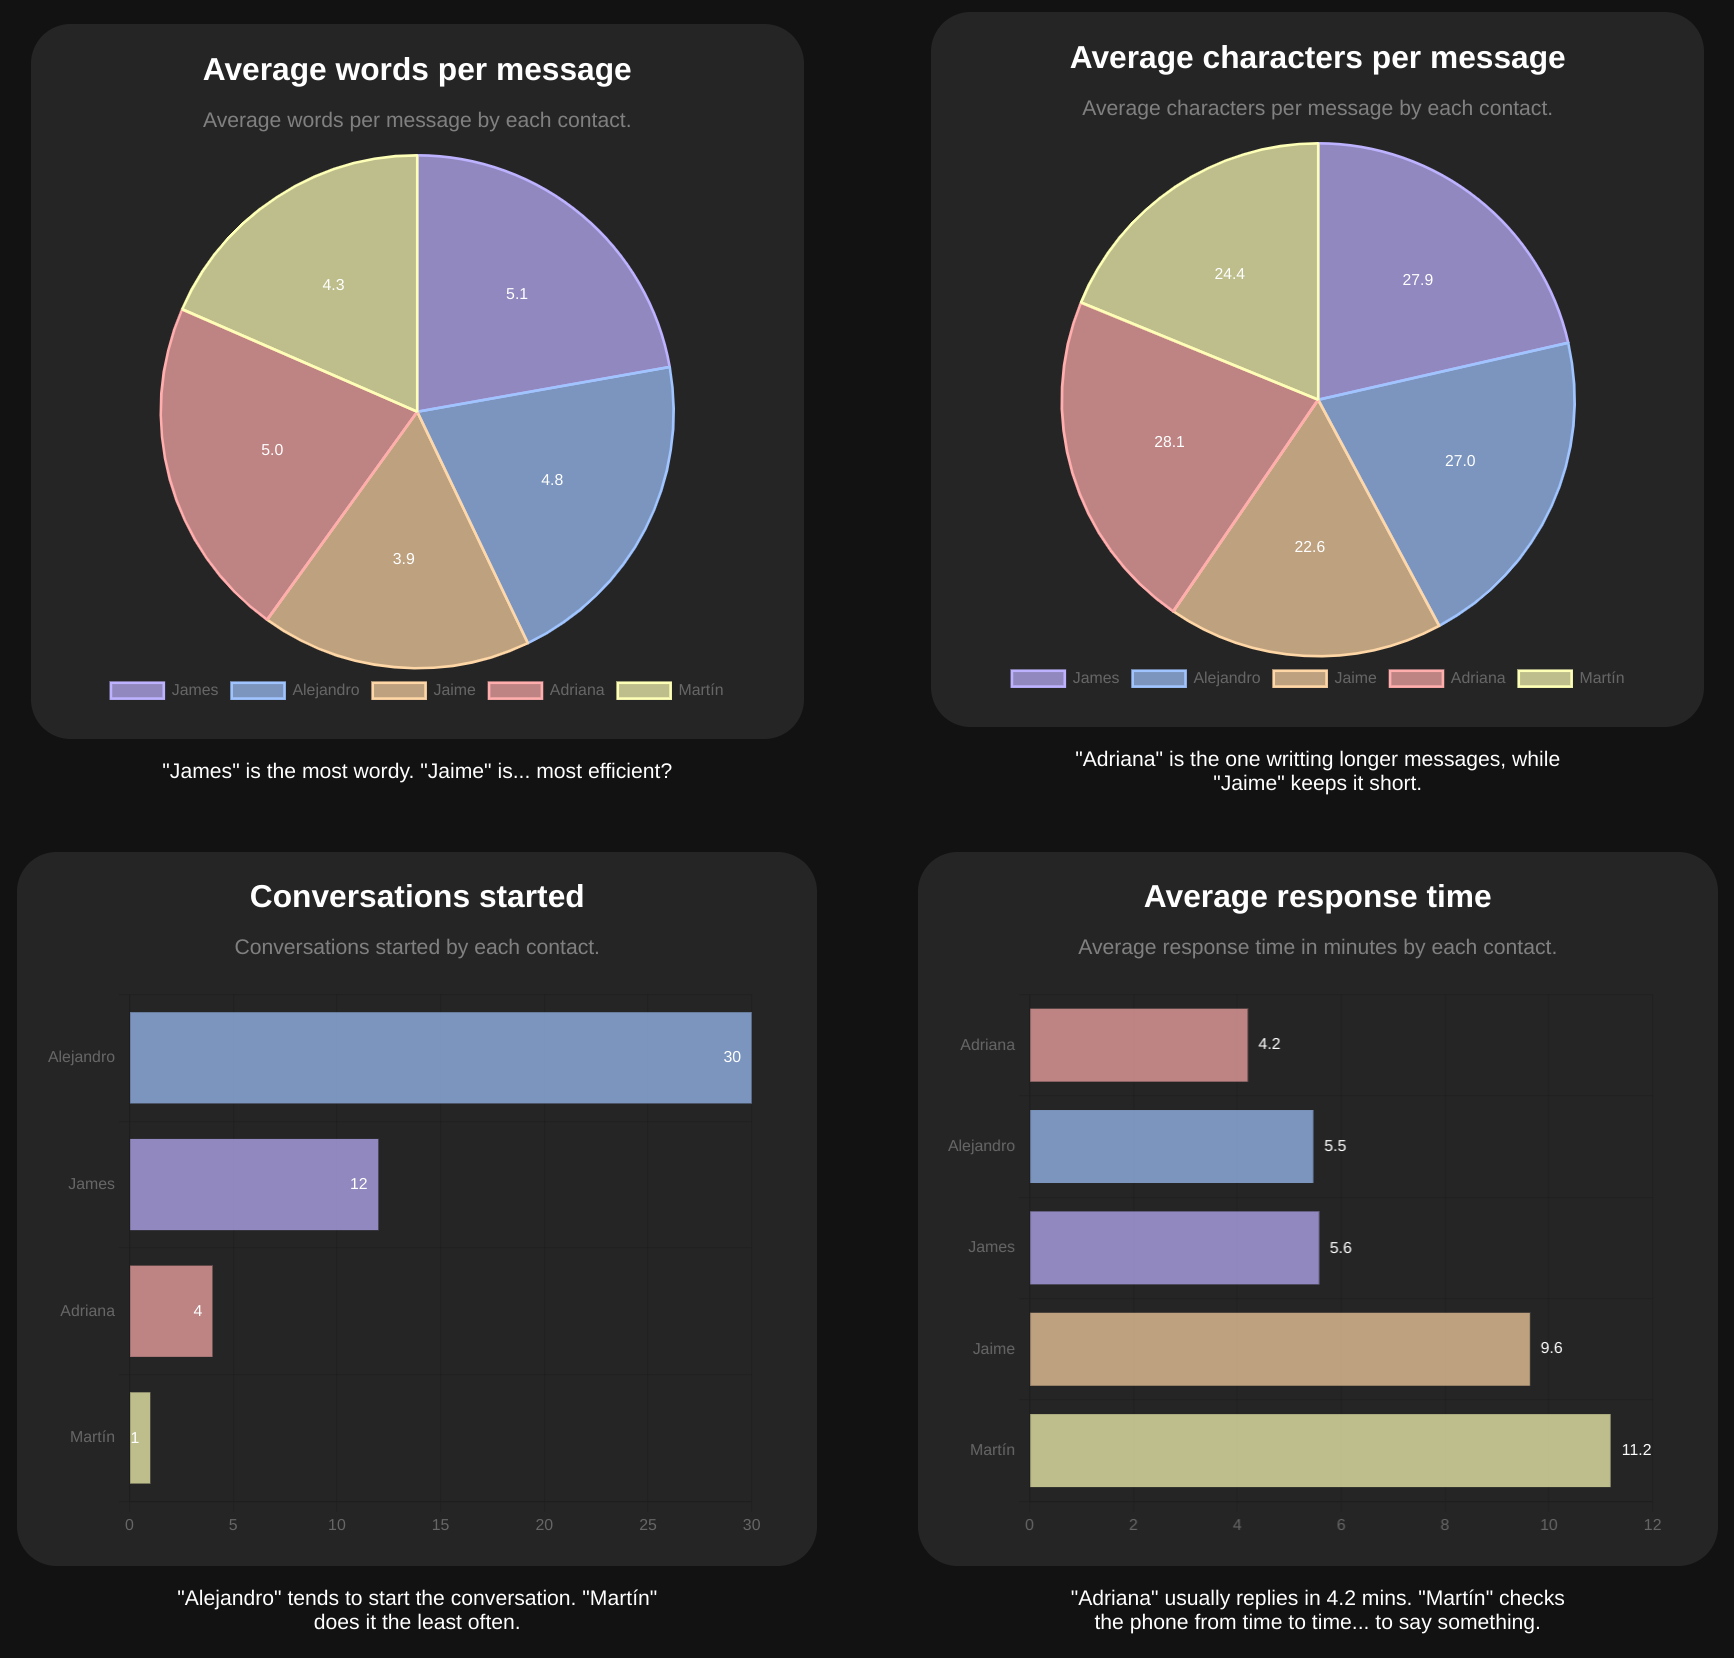
\includegraphics[width=7cm]{img/study_case/screen_2.png} }}
	\centering
	
	
	\subfloat[\centering Número de fotos, vídeos, audios y pegatinas]{{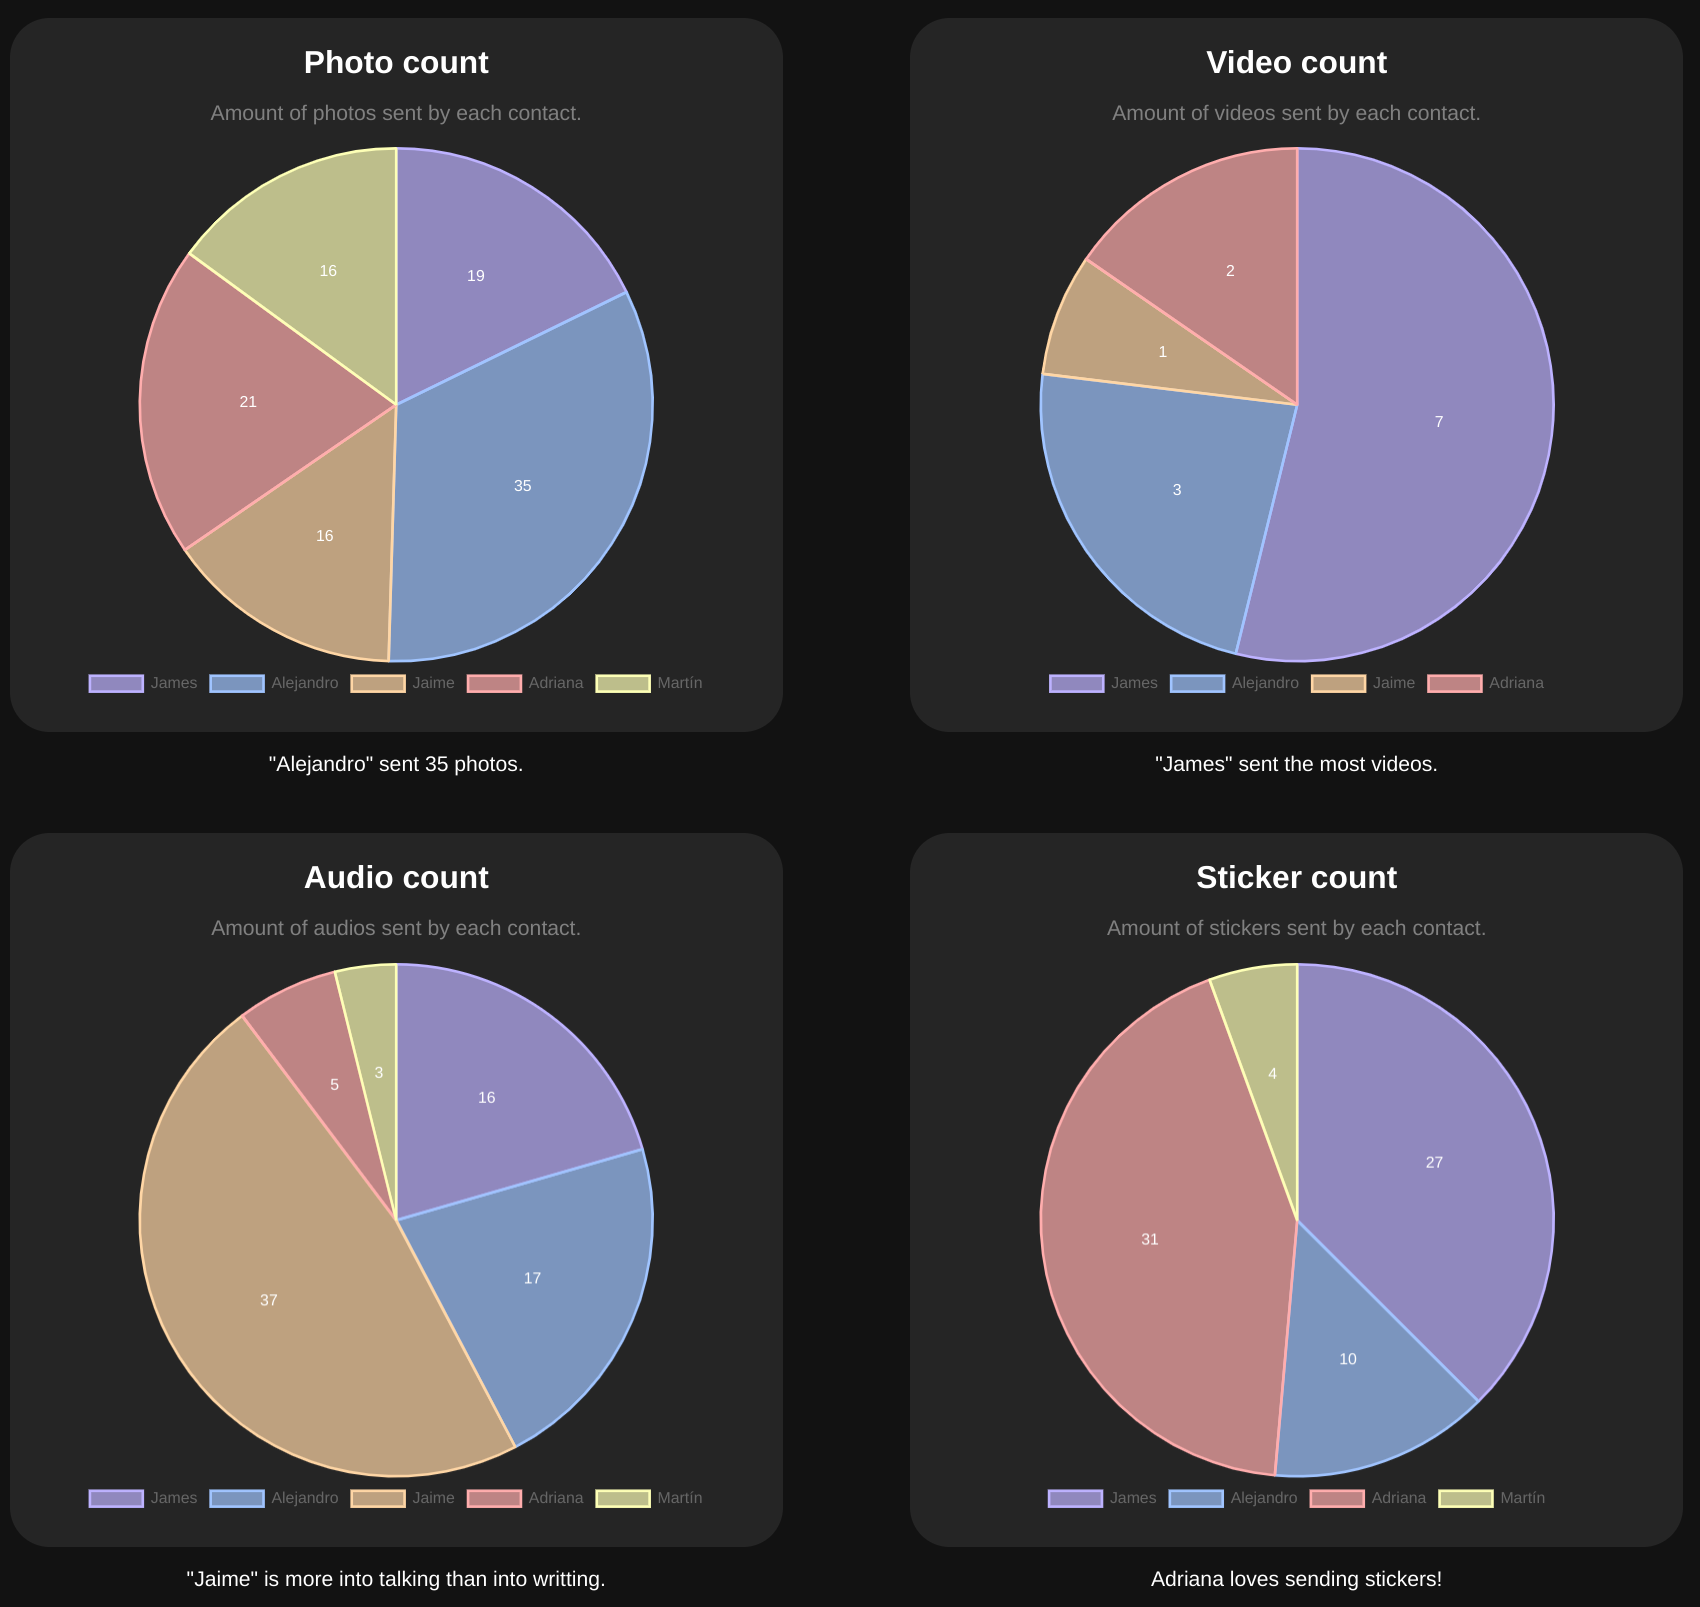
\includegraphics[width=7cm]{img/study_case/screen_3.png} }}
	\qquad
	\subfloat[\centering Distribución de mensajes en meses, días de la semana y  horas del día]{{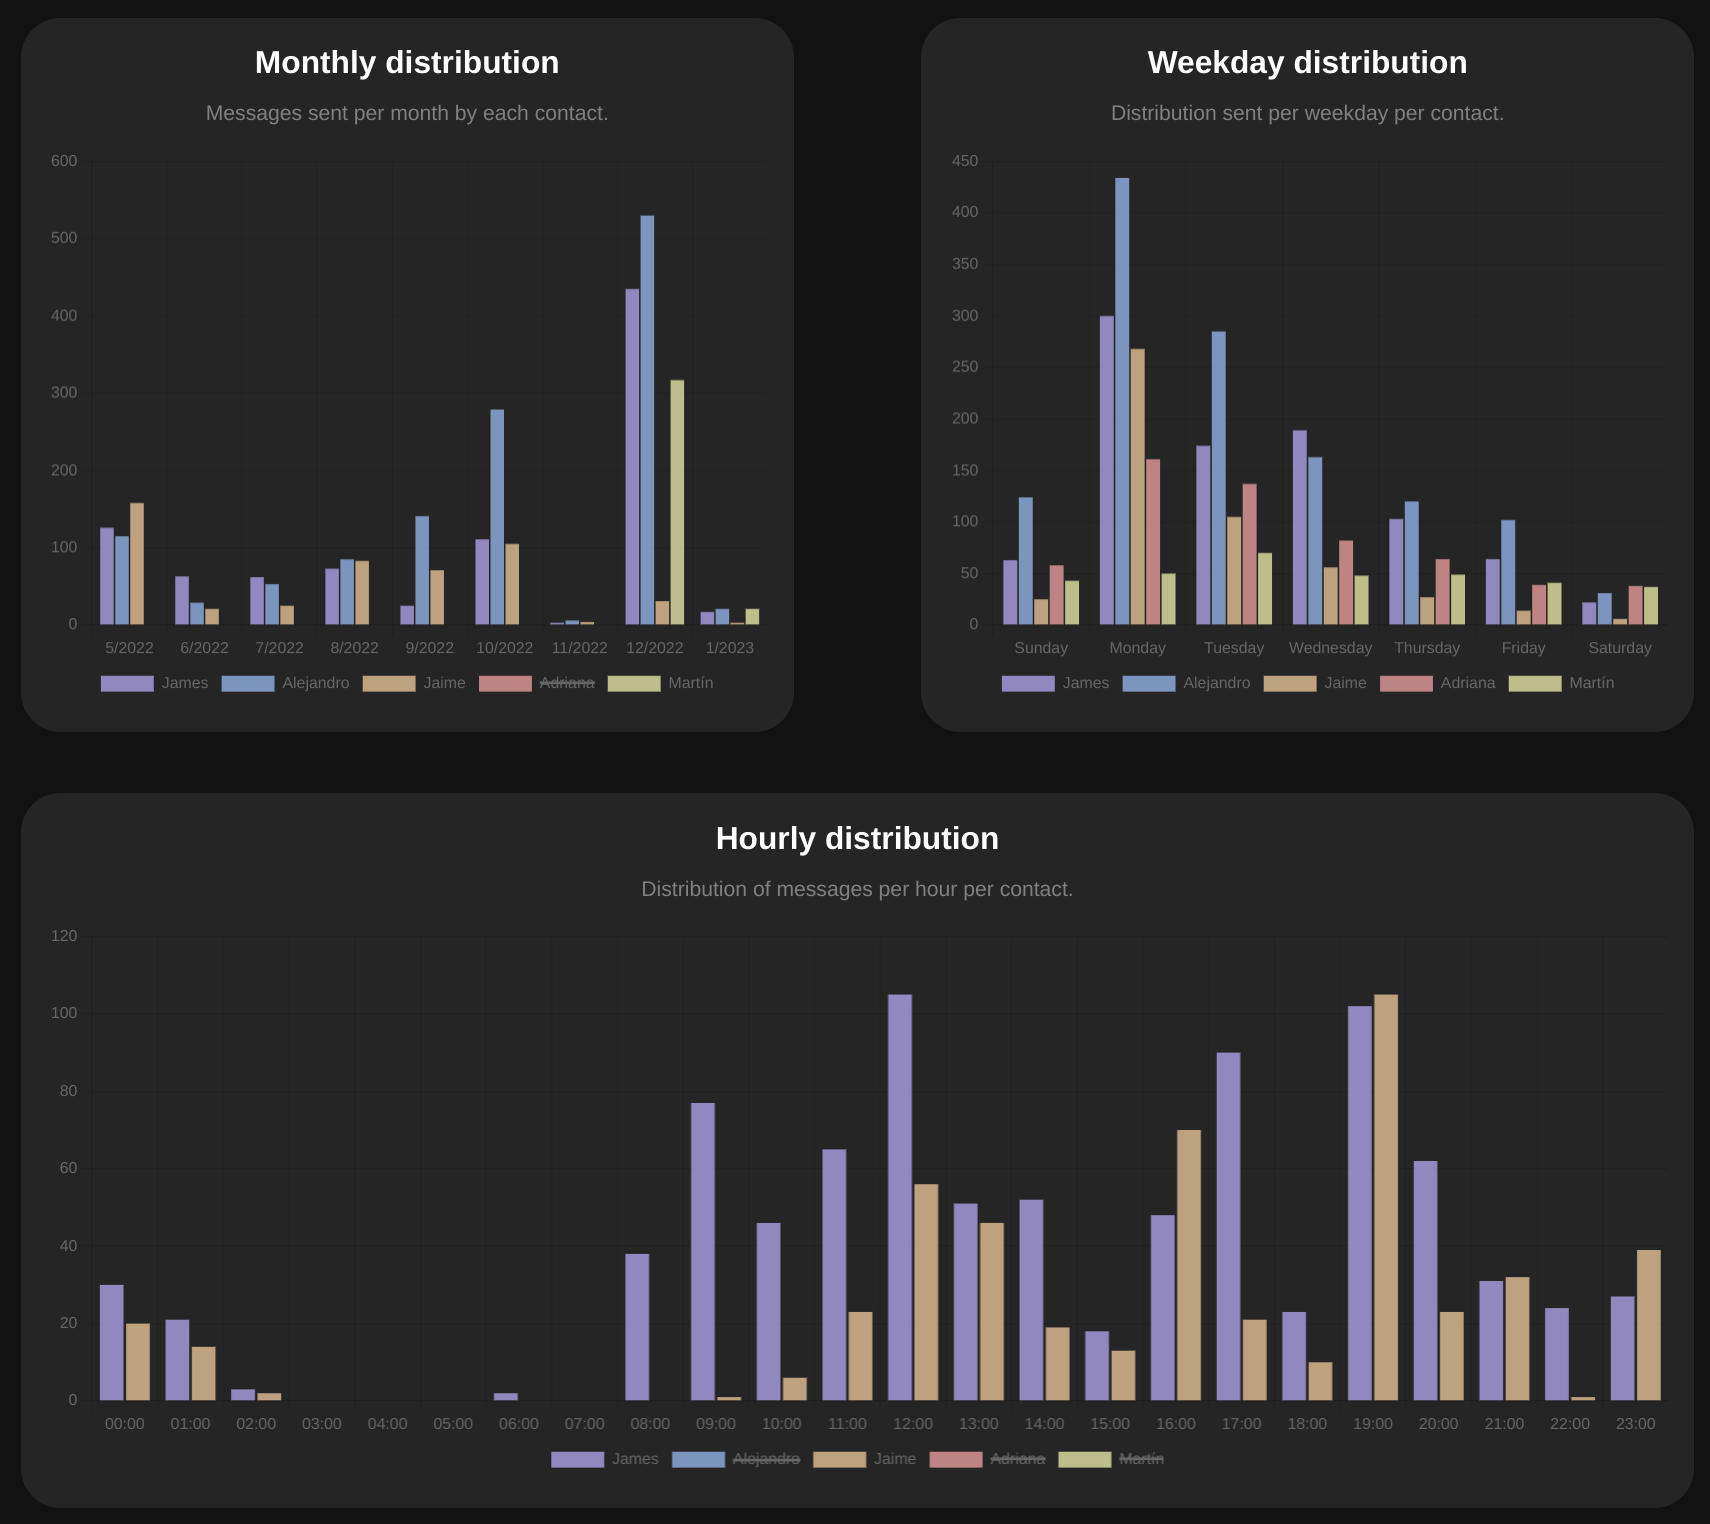
\includegraphics[width=7cm]{img/study_case/screen_4.png} }}
	
	
	\qquad
	\subfloat[\centering Nubes de palabras y emoticonos]{{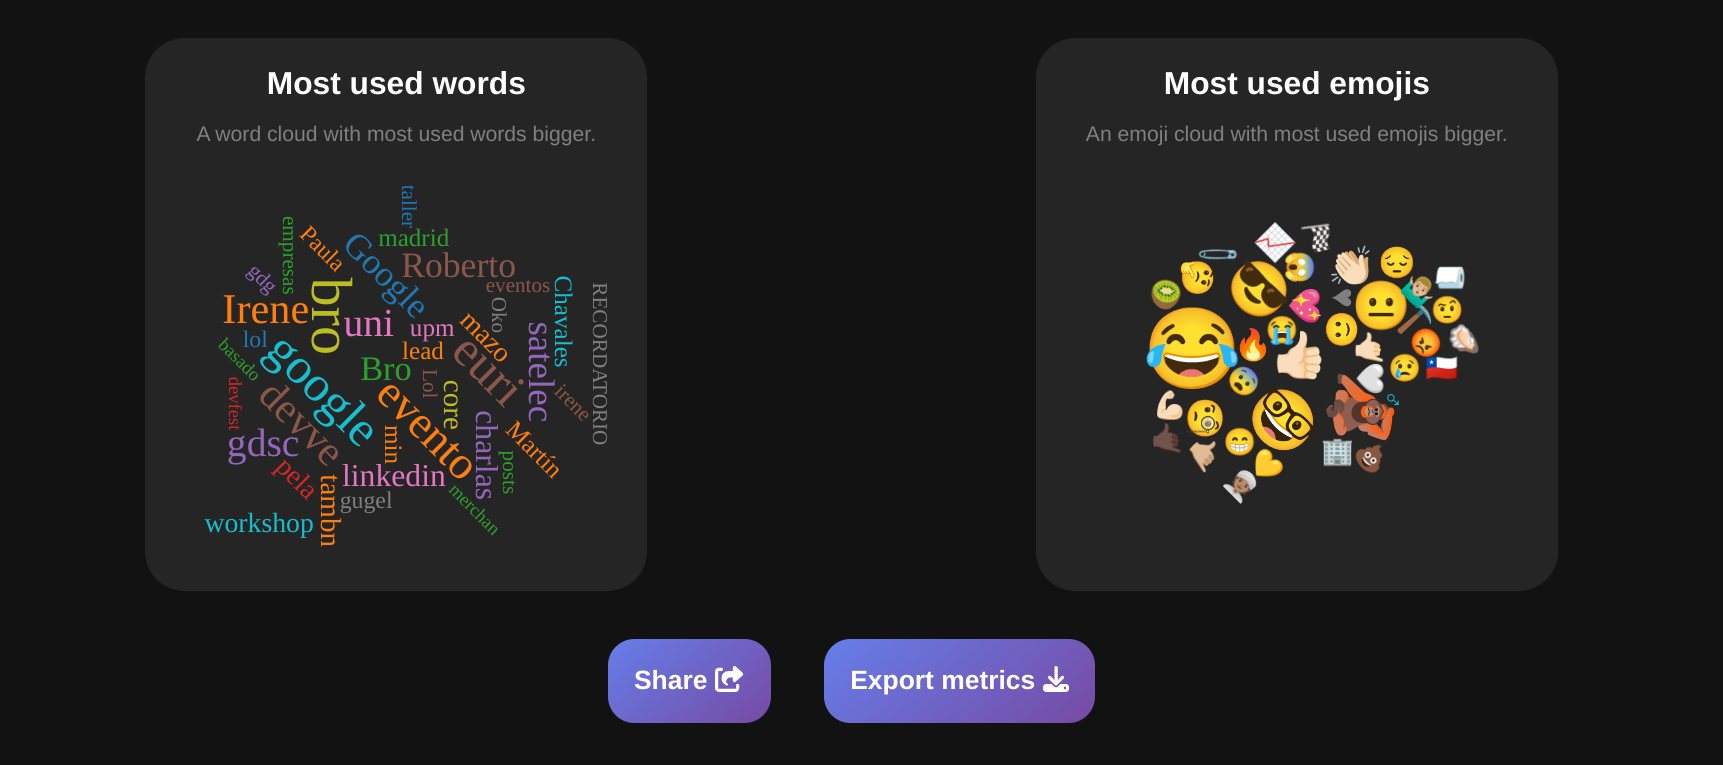
\includegraphics[width=9cm]{img/study_case/screen_5.png} }}
	
	
	\caption{Visualización de chat grupal}
	\label{fig:chap5:viz_grupal}
\end{figure}


\begin{figure}[h]
	\centering
	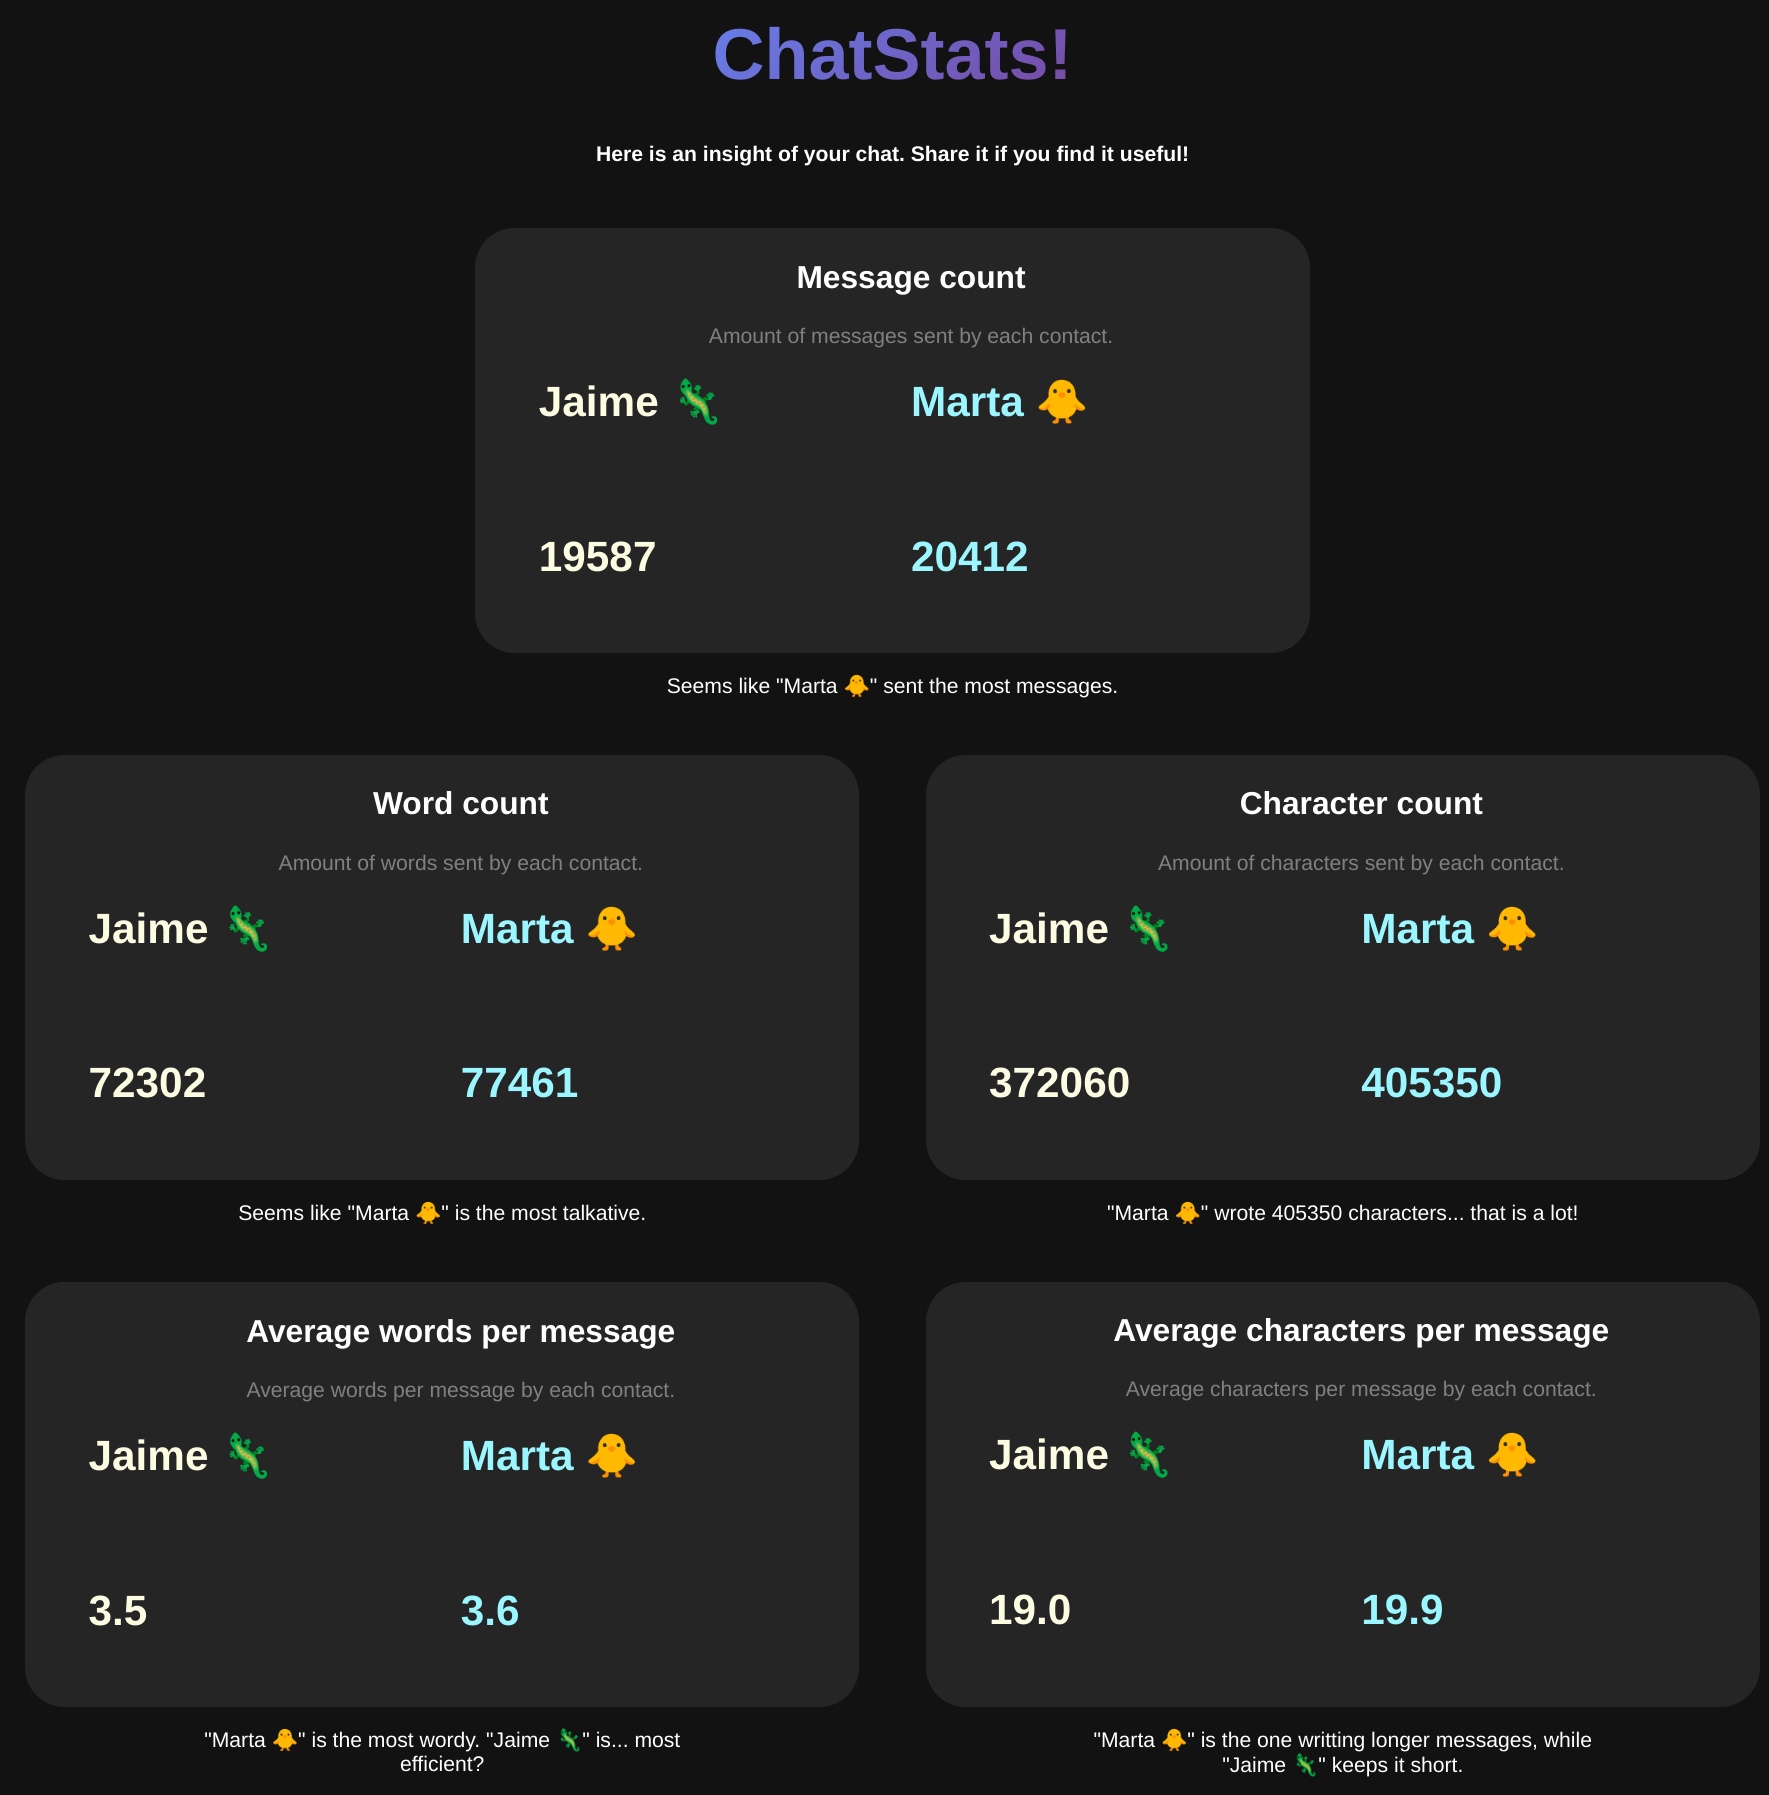
\includegraphics[width=0.8\textwidth]{img/study_case/screen_6.png}
	\caption{Ejemplo de variación para chat individual}
	\label{fig:chap5:viz_individual}
\end{figure}

\section{Exportar analíticas}

Como puede observarse en la \autoref{fig:chap5:export}, se ofrece la opción, al final de la visualización, de exportar una imagen para compartir; así como de exportar las métricas calculadas para su posterior análisis personal.

\begin{figure}[h]
	\centering
	\subfloat[\centering Compartir imagen]{{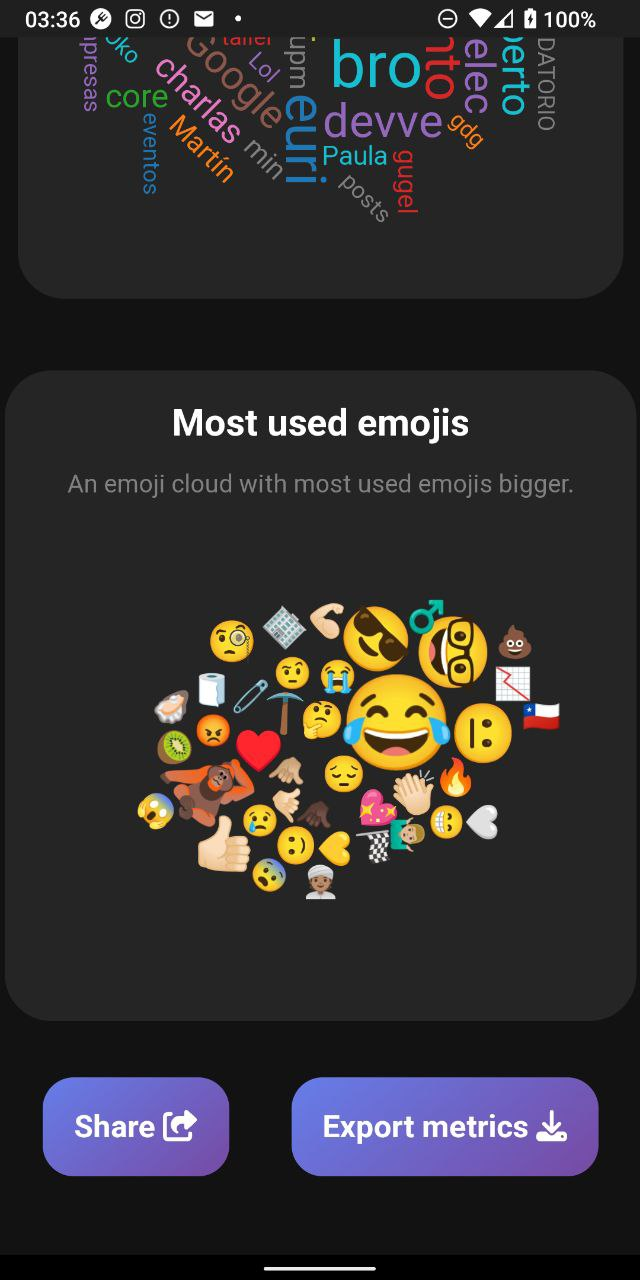
\includegraphics[width=5cm]{img/study_case/export_1.jpg} }}
	\qquad
	\subfloat[\centering Descarga del archivo exportado]{{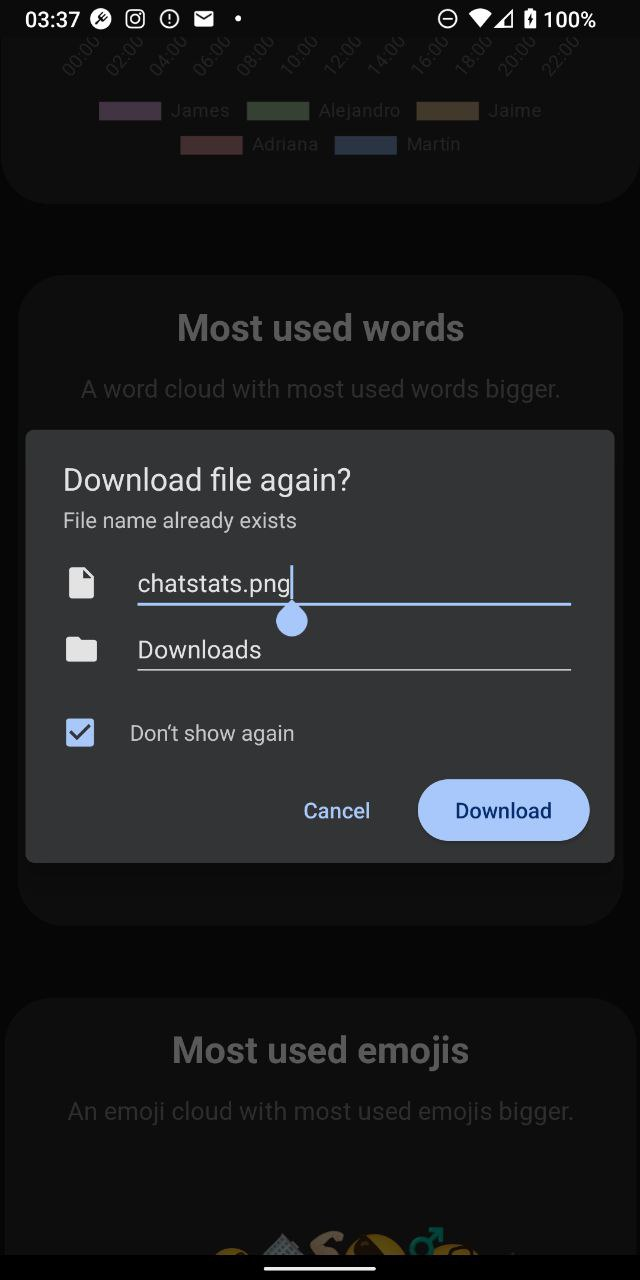
\includegraphics[width=5cm]{img/study_case/export_2.jpg} }}
	\caption{Exportar analíticas}
	\label{fig:chap5:export}
\end{figure}
\chapter{Conclusiones y futuras líneas de trabajo}
\label{chap:conclusions}

En este capítulo se exponen las conclusiones extraídas del proyecto, así como recomendaciones y posibles futuras líneas de trabajo.

\section{Conclusiones}
\label{sec:conclusions}

Académicamente, este proyecto ha desarrollado una doble función: la de proyecto personal y, la de trabajo de fin de grado.

La motivación principal del proyecto era desarrollar una aplicación web para ayudar a analizar conversaciones de WhatsApp, permitiendo detectar y mejorar los problemas encontrados; y este pro

\begin{comment}
	
Academically, this Project served a double purpose: learning about statistics and machine learning and developing a method for improving the accuracy of an existing system.

The initial motivation for the Project was to develop better estimations for the bus \acrshort{eta}s, and this main objective has been satisfactorily accomplished. Precisely, both of the goals proposed in the introduction (characterizing the \acrshort{crtm} \acrshort{api} estimations and developing alternative estimators) have been fullfilled.

The first step was to review the existing bibliography and check the available data and data sources from the \acrshort{crtm}. Then, we addressed the first challenge: obtaining as much data about the buses mobility as possible without saturating the \acrshort{crtm} \acrshort{api} server. After several tests, the server behaviour was characterized and decisions for an optimal data gathering were taken. Furthermore, the Python package \textbf{crtm\_poll} was developed for automating the server polling process. As a conclusion, the optimization of the data acquisition procedures is crucial in this type of scenarios.

Once the data was available, a data analysis environment was set up for its processing. An algorithm for estimating the bus passing time from the \acrshort{api} provided \acrshort{eta}s was designed, which involved filtering the raw data obtained from the \acrshort{crtm} \acrshort{api}. Knowing the arrival times of past trips, the running time between stops could be obtained and a web visualization tool was developed for displaying them. The developed tools allowed to visually detect some fundamental behavior patterns in the mobility of the buses.

Next, alternative estimators for the running times between stops and for the bus \acrshort{eta} to a stop were designed. For that purpose different statistical tools and machine learning models were employed. Our experience indicates that although the available software for machine learning model design is very powerful, a clear understanding of the addressed problem and of the training schemes is required to be able to correctly interpret the results.

Concerning the developed tools, the running time between stops estimators developed in Section \ref{running_time_between_two_stops} could be used to improve the accuracy of the estimations made by the \acrshort{crtm} \acrshort{api} or by other source of estimators; in general, they can also be applied to any scenario where we want to estimate the running time between two points of a vehicle following a fixed route.

The relevant idea behind the estimator developed in Section \ref{reamining_time_at_anytime} is that it can be understood as a system that corrects the estimations provided by another system. This could be an easy to implement solution for improving the accuracy of the estimations made by more complex systems just by setting it prior to them.

The main limitation for implementing the proposed online estimator is the bottleneck produced by the \acrshort{crtm} \acrshort{api} server, which would not be able to handle all the needed requests for sampling all the bus stops at the same time. Nevertheless, the computational cost of each of the used models was calculated in case that the processing capacity requirements were to be consider for a future implementation.

In general, the developed methods in this Project are built in a way that allows the usability for other similar use cases. The hyperparameters of the estimators are chosen based on the data and the available input features, so they can be easily adapted for different system behaviors.
\end{comment}

\section{Objetivos conseguidos}
\label{sec:achieved-goals}
\begin{description}
	
\item Creación de una aplicación web.
\item Compatibilidad con \acrfull{pwa}.
\item Compatibilidad con datos de conversaciones grupales e individuales.
\item Compatibilidad con datos de conversaciones con y sin contenido multimedia.
\item Compatibilidad con todos los formatos de exportación de la aplicación WhatsApp para distintos sistemas operativos.
\item Cálculo de estadísticas generales de los datos.
\item Visualizaciones gráficas para los distintos estadísticos.
\item Posibilidad de interacción con los gráficos.
\item Implementación de tests para estabilidad y comprobación del código fuente.

\end{description}

\section{Futuras líneas de trabajo}
\label{sec:future-work}

\begin{itemize}

\item Migración de los módulos con mayor carga de trabajo a \acrfull{wasm}, permitiendo obtener un rendimiento mayor y cercano al nativo del cliente que ejecuta la aplicación.

\item Mayor facilidad para añadir módulos, mediante un sistema de carpetas y plugins.

\item Inclusión de visualizaciones para el análisis de sentimientos y su evolución en el tiempo.

\item Añadir soporte para otras plataformas de mensajería como Telegram.

\item Implementación de \textit{cache} en la \acrfull{pwa} para poder ejecutar la aplicación sin necesidad de acceso a Internet (una vez instalada).

\item Mejora de la documentación para futuros contribuyentes al proyecto.

\end{itemize}


\cleardoublepage
\pagenumbering{roman}
\appendix
\begin{appendices}
    \chapter{Impacto del proyecto} \label{chap:impact}

\section{Impacto social} \label{sec:social_impact}

\subsection{Introducción}

Este proyecto aporta herramientas para el estudio y análisis de las relaciones personales llevadas a cabo mediante las aplicaciones WhatsAp y Telegramp, permitiendo evaluar y mejorar y tomar decisiones las mismas mediante la observación de los resultados.

\subsection{Descripción de impactos relevantes relacionados con el proyecto}

El cuidado de las comunicaciones que tienen lugar a través de WhatsApp puede ayudar a las personas a dedicar el tiempo necesario a mantener relaciones saludables y darse cuenta de posibles fallos que están teniendo lugar en la comunicación a largo plazo, o analizar su comportamiento.

Otro impacto relevante a la ética del proyecto es las consideraciones de privacidad en un tema tan importante como son las conversaciones privadas del usuario, que se ha considerado prioritario durante las decisiones de diseño y arquitectura.

\subsection{Conclusiones}

Las consideraciones sociales de este proyecto son el núcleo del desarrollo del mismo, así como la causa por la que el proyecto comenzó en un primer lugar.
    \chapter{Presupuesto económico} \label{chap:economic}

\section{Costes}

\ \hfill
\begin{tabular}{ p{5.5cm}|p{2.7cm}|p{2.7cm}|p{2cm}|  }
	\cline{2-4}
	& \multicolumn{3}{|c|}{\textbf{COSTE DE MANO DE OBRA (coste directo)}} \\
	\cline{2-4}
	& Horas & Precio/hora & Total \\
	\cline{2-4}
	& 360 & \hfill 12 \euro & \hfill 4,320.00 \euro \\
	\cline{2-4}
\end{tabular}

\vspace{1cm}

\ \hfill
\begin{tabular}{ |p{3cm}| *{4}{p{2.1cm}|}  }
	\hline
	\multicolumn{5}{|c|}{\textbf{COSTE DE RECURSOS MATERIALES (coste directo)}} \\
	\hline
	& Precio de compra & Uso en meses & Amortización (en años) & Total \\
	\hline
	Portátil personal & \hfill 1,500.00 \euro & 6 & 5 & \hfill 150.00 \euro \\
	\hline
	Tablet & \hfill 1,099.00 \euro & 6 & 5 & \hfill 109.90 \euro \\
	\hline
	\multicolumn{4}{|l|}{COSTE TOTAL DE RECURSOS MATERIALES} & \hfill 259.90 \euro \\
	\hline
\end{tabular}

\vspace{1cm}

\ \hfill
\begin{tabular}{ |p{8.4cm}|p{0.8cm}|p{2.1cm}|p{2cm}| }
	\hline
	\textbf{GASTOS GENERALES (costes indirectos)} & 15\% & de CD & \hfill 686.98 \euro \\
	\hline
	\textbf{BENEFICIO INDUSTRIAL} & 6\% & of CD+CI & \hfill 316.01 \euro \\
	\hline
\end{tabular}

\vspace{1cm}

\ \hfill
\begin{tabular}{ |p{5cm}|p{2cm}|  }
	\hline
	\multicolumn{2}{|c|}{\textbf{MATERIAL FUNGIBLE}} \\
	\hline
	Impresión y encuadernación & \hfill 50.00 \euro \\
	\hline
\end{tabular}

\vspace{1cm}

\ \hfill
\begin{tabular}{ |p{4cm}|p{2cm}|p{2cm}|  }
	\hline
	\multicolumn{2}{|l|}{\textbf{PRESUPUESTO SUBTOTAL}} & \hfill 5,632.89 \euro \\
	\hline
	\textbf{IVA APLICABLE} & 21\% & \hfill 1,182.91 \euro \\
	\hline
\end{tabular}

\vspace{1cm}

\ \hfill
\begin{tabular}{ |p{5cm}|p{2cm}|}
	\hline
	\textbf{PRESUPUESTO TOTAL} & \hfill 6,815.80 \euro \\
	\hline
\end{tabular}

    \chapter{Código} \label{chap:code}

\section{Acceso al código fuente}

Acceso principal: \url{https://codeberg.org/devve/chatstats}

Copia (mirror): \url{https://github.com/d3vv3/chatstats}


    \chapter{Expresiones regulares} \label{chap:regex}

En este anexo se exponen los distintos grupos de captura que definen la expresión regular para el parseo de chats exportados por WhatsApp, tanto desde Android como iOS.

\begin{figure}[h]
	\centering
	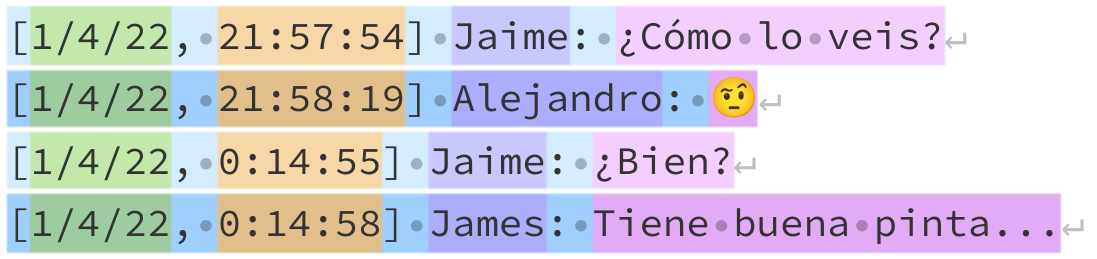
\includegraphics[width=0.8\textwidth]{img/regex_ios.png}
	\caption{Grupos de captura iOS en color}
	\label{fig:chap:regex_ios}
\end{figure}

\begin{figure}[h]
	\centering
	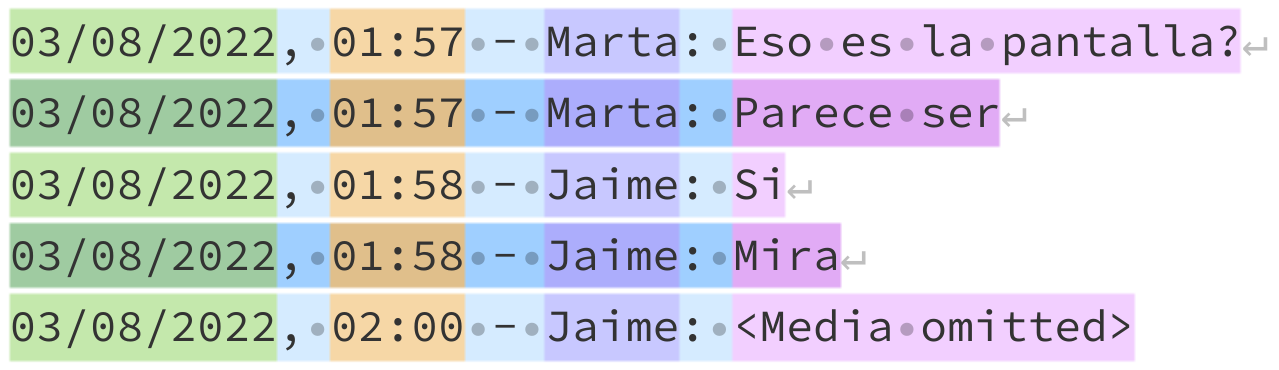
\includegraphics[width=0.8\textwidth]{img/regex_android.png}
	\caption{Grupos de captura Android en color}
	\label{fig:chap:regex_android}
\end{figure}

\section{Grupos de captura}

Como se decribe en el \autoref{chap:architecture}, poder separar cada mensaje se ha llegado a la siguiente expresión regular, cuyos grupos se explicaran a continuación:

\begin{lstlisting}
	/\[*(\d{1,2}\/\d{1,2}\/\d{2,4}),\s(\d{1,2}:\d{2}:*\d*)\]*\s(?:-\s)*(.*?):{1}\s(.*?)(?=\s\[*\d{1,2}\/\d{1,2}\/\d{2,4}|$)/gum
\end{lstlisting}

Se denotan los distintos grupos de captura por las agrupaciones realizadas con los paréntesis. Se exponen:

\paragraph{Grupo de captura 1: fecha}\mbox{}\\

\begin{lstlisting}
	(\d{1,2}\/\d{1,2}\/\d{2,4})
\end{lstlisting}

Se encarga de la fecha en formato \textit{dd/mm/YYYY} para Android y \textit{d/m/YY} para iOS; denotado con ``$\backslash d\{X,Y\}$'' que indica que se buscan entre $X$ e $Y$ dígitos de $0$ a $9$ seguidos, separados por un ``$/$''. En las expresiones regulares hay que escapar los ``$/$'' o \textit{slash} con un ``$\backslash$'' o \textit{backslash}.

Durante numerosas pruebas, se ha observado que no hay consistencia entre los ajustes del parámetro \textit{locale} de \textit{en\_US} y \textit{es\_ES}, siendo \textit{mm/dd/YYY} y \textit{dd/mm/YYYY} respectivamente. Para ello, ChatStats accederá al \textit{locale} para actuar en consecuencia más adelante. No se ha probado para otras configuraciones.

Puede observarse en verde en la \autoref{fig:chap:regex_android} y \autoref{fig:chap:regex_ios}.

\paragraph{Grupo de captura 2: hora}\mbox{}\\

\begin{lstlisting}
	(\d{1,2}:\d{2}:*\d*)
\end{lstlisting}

Se encarga de la la hora en formato \textit{hh:MM} para Android y \textit{h:M:ss} para iOS, donde en caso de comenzar por 0, este no se muestra. Es por ello que se esperan entre 1 y 2 dígitos para la hora y los minutos, así como el parámetro de los segundos es opcional. Este último parámetro, si existe, siempre está conformado por dos números.

Puede observarse en naranja en la \autoref{fig:chap:regex_android} y \autoref{fig:chap:regex_ios}.

\paragraph{Grupo de captura 3: contacto}\mbox{}\\

\begin{lstlisting}
	(.*?)
\end{lstlisting}

Se encarga del nombre del contacto. Busca la repetición de caracteres ilimitados a excepción del carácter ``\textit{:}'', ya que éste es un separador.

Puede observarse en azul oscuro en la \autoref{fig:chap:regex_android} y \autoref{fig:chap:regex_ios}.

\paragraph{Grupo de captura 4: mensaje}\mbox{}\\

\begin{lstlisting}
	(.*?)
\end{lstlisting}

Se encarga del cuerpo del mensaje. Busca la repetición de caracteres ilimitados, incluyendo caracteres unicode para tener los emoticonos en cuenta. Esta búsqueda de caracteres se realiza de manera perezosa, expandiendo las coincidencias en caso posible, siempre que no coincida con el siguiente grupo de captura (\textit{lookahead}).

Puede observarse en rosa en la \autoref{fig:chap:regex_android} y \autoref{fig:chap:regex_ios}.

\paragraph{Look ahead o mirada hacia delante}\mbox{}\\

\begin{lstlisting}
	(?=\s\[*\d{1,2}\/\d{1,2}\/\d{2,4}|$)
\end{lstlisting}

Si únicamente contáramos con el grupo de captura 4, solo se reconocería el primer mensaje, puesto que se reconocería el resto del texto como cuerpo del primer mensaje. Para solucionarlo, en el grupo de captura 4 se intentan reconocer el menor número posible de coincidencias, hasta el siguiente patrón reconocido. Este patrón es una mirada hacia delante conformada por la misma expresión regular que en el grupo de captura 1.

\paragraph{Opciones}\mbox{}\\

\begin{lstlisting}
	\gum
\end{lstlisting}
 
Finalmente se aplican tres opciones a la expresión regular, que son:

\begin{itemize}
	\item \textbf{g:} Nos permite no terminar la búsqueda de patrones tras la primera coincidencia.
	\item \textbf{u:} Nos permite la búsqueda de caracteres unicode, así como emojis (que pertenecen a la especificación unicode).
	\item \textbf{m:} Nos permite realizar la búsqueda en numerosas líneas, pudiendo encontrar coincidencias con mensajes de varias líneas.
\end{itemize}
    \chapter{Formato de mensajes exportados por Telegram}
\label{chap:telegram_json}

Se expone a continuación un breve ejemplo del formato utilizado por Telegram para la exportación de sus chats, que es el mismo para chats individuales y grupales.

\begin{lstlisting}[language=JavaScript]
	{
		"name": "group_or_contact_name",
		"type": "private_group_or_private_chat",
		"id": 00000000,
		"messages": [
		...
		{
			"id": 11111,
			"type": "message_service",
			"date": "2019-04-02T20:53:14",
			"date_unixtime": "1554231194",
			"from": "Alice",
			"from_id": "contact_user_id",
			"text": "actual_body_message",
			"text_entities": [
			{
				"type": "plain_link_or_document",
				"text": "actual_body_message"
			}
			]
		},
		{
			"id": 22222,
			"type": "message",
			"date": "2019-05-29T23:46:00",
			"date_unixtime": "1559166360",
			"from": "Bob",
			"from_id": "contact_user_id",
			"reply_to_message_id": 59386,
			"file": "stickers/sticker.webp",
			"thumbnail": "stickers/sticker.webp_thumb.jpg",
			"media_type": "sticker",
			"sticker_emoji": "actual_unicode_emoji",
			"width": 512,
			"height": 341,
			"text": "",
			"text_entities": []
		}, ...
		]
	}
\end{lstlisting}
\end{appendices}

\cleardoublepage
\phantomsection
\nocite{*}
\addcontentsline{toc}{chapter}{Bibliography}   % ieeetr
\bibliographystyle{unsrt}
\bibliographystyle{plain}{
    \small
    \bibliography{biblio/ref}
}

\end{document}